%!TEX root = ../../../thesis.tex
\chapter{Network Analysis}\label{chap:analysis}

	We present a systematic study of the characteristic vein networks formed by the slime mold \P. Our study is based on an extensive set of graph representations of slime mold networks. We analyze a total of $1998$ graphs capturing growth and network formation of \P as observed in $36$ independent, identical, wet-lab experiments. Relying on concepts from graph theory such as face cycles and cuts as well as ideas from percolation theory, we establish a broad collection of individual observables taking into account various complementary aspects of \P networks. As a whole, the collection is intended to serve as a specialized knowledge-base providing a comprehensive characterization of \P networks. To this end, it contains individual as well as cumulative results for all investigated observables across all available data series, down to the level of single \P graphs. Furthermore we include the raw numerical data as well as various plotting and analysis tools to ensure reproducibility and increase the usefulness of the collection. All our results are publicly available in an organized fashion in \SMGR introduced in \Fref{chap:smgr}.
	
	This chapter presents joint work with Prof.~K.~Mehlhorn~\cite{dirnberger2016}.

\section{Introduction}		

	Networks are systems consisting of nodes and links. In general, nodes represent abstract entities while links define abstract relationships between them. Once one adopts this powerful concept, networks appear virtually everywhere throughout nature and as systems created by men.

	Man-made examples include networks of servers such as the Internet~\cite{faloutsos1999power,karagiannis2004long,huberman1999internet}, networks of web-pages~\cite{adamic2000power}, networks of streets~\cite{jiang2004topological,buhl2006topological}, power grids~\cite{rohden2012self,zhongwei2004comparison} or transportation networks involving trains or air planes~\cite{barrat2004weighted,guimera2004modeling,sienkiewicz2005statistical,sen2003small}. Examples for networks observed in nature include gene regulation networks~\cite{alon1999robustness,milo2002network}, food webs~\cite{pimm1991food,montoya2006ecological}, fungal cord networks~\cite{fricker2007network,heaton2012analysis}, or vascularization networks in plants and mammals~\cite{katifori2010damage,roth2001evolution,koizumi2000series}, to name but a few. 

	A property shared by many networks is that they are \emph{complex}. While an unambiguous definition of the term is elusive, complex networks share some common characteristics. They typically consist of a large number of nodes exhibiting possibly unknown, non-trivial interactions. The network itself as well as the interactions between its constituents are not constant but subject to change induced by internal or external events. Furthermore, self-organization and emergent phenomena are commonly observed in complex networks~\cite{barabasi1999emergence,boccaletti2006complex}.

	Given the intellectual challenges and the importance of technical applications associated with complex networks, research concerned with their structure and function has attracted continuing scientific interest. For extensive reviews and references on the topic consult~\cite{newman2003structure,boccaletti2006complex,strogatz2001exploring,amaral2004complex}.

	The present article focuses on vein-networks formed by the unicellular, multi-nucleated slime mold \Pp~\cite{lifecycle}. This peculiar amoeba-like organism is able to maintain a massive cell body in the form of an extended network of veins. Similar to a mammalian vascular network, the veins carry protoplasmic fluid distributing nutrients and other matter throughout the cell body by means of peristaltic pumping~\cite{kamiya1959motive}. \P reacts to changing environmental conditions by dynamically adapting the topology of its network. In the absence of a central nervous system capable of coordinating morphological changes in \P, it is believed that the ability to reorganize itself to better meet environmental conditions is an emergent property resulting from underlying local interactions~\cite{tero2010rules,nakagaki2007minimum}.

	In order to further improve our understanding of the mechanisms governing the morphology of \P one may directly study the properties of its networks. A popular two-step approach, consists of capturing images of networks and converting them to mathematical graphs, enabling a detailed investigation of their properties~\cite{baumgarten2012computational}. The first part relies on cultivating \P in the lab whilst taking images that document the development of the organism and its networks. The second part requires dedicated methods capable of analyzing the obtained images and computing graph representations of the networks depicted therein. Such methods have become available as software packages recently~\cite{dirnberger2015nefi}. Once graphs have been established, methods from graph theory and network science apply and various quantities of interest can be computed. This approach has been quite successful and various interesting network properties have been established~\cite{baumgarten2010plasmodial,baumgarten2013functional,ito2011characterization}, however, many questions remain open.

	In this chapter we continue to investigate \P using the graph-based approach. Our study relies on a publicly available set of \P graphs which is part of the \SMGR~\cite{SMGR}, see \Fref{chap:smgr}.

	Based on the \data, we define and compute a broad collection of observables characterizing \P graphs. We begin our investigation by reporting a suite of basic graph properties and discuss our findings in relation to results obtained prior to our study~\cite{baumgarten2010plasmodial}. We proceed by introducing a family of observables using concepts from graph theory such as face cycles and cuts. Finally, we study the robustness of \P networks under random attack by establishing edge and node percolation thresholds. 

	We seek to establish a broad spectrum of descriptive observables designed to cover various complementary aspects of the organism. The combination of these may be interpreted as a kind of multidimensional ``fingerprint'' capable of characterizing \P graphs. Using such fingerprints, it becomes possible to compare individual \P graphs in a quantitative manner. This can be of particular use when comparing different slime molds with each other or in the evaluation of models or algorithms producing graphs which claim properties similar to those of \P. Our approach nicely complements recent efforts to compare different slime molds based on properties of their plasmodia and certain chemotactic responses~\cite{westendorf2016quantitative}.

	We stress that this manuscript only provides an overview of our findings. The complete set of results is available for download and inspection at the \href{http://smgr.mpi-inf.mpg.de}{SMGR}. This includes the full list of observables and associated plots, useful tools as well as instructions that allow the reproduction of all obtained results. Crucially, the provided tools enable the reader to define and compute new observables tailored to their particular research questions.

	Establishing a broad body of reliable information and making it available together with useful tools are the major goals of our efforts. We hope that they will serve as a catalyst for future research.

\section{Methods}

	\subsection{Experimental data}

		To investigate the properties of networks formed by \P we rely on experimental data publicly available in the \SMGR. The \SMGR was introduced recently in an effort to improve the visibility and reuse of experimental data with a focus on slime mold networks and their graph representations.
	
		For the present study we work with the \href{http://smgr.mpi-inf.mpg.de}{SMGR}'s initial data set, called the \data. In particular we focus on a processed subset of this data tagged \emph{high unfiltered}. For a detailed account on how this data was obtained (experimental setup and procedures), processed (raw images, network extraction and filtering, relevant implementations) and organized we refer to \Fref{chap:smgr}. 

		Here it suffices to say that the \data contains time series of mathematical graphs derived from images depicting growth and network formation of \P as observed in $36$ independent, identical, wet-lab experiments. Note that no additional food sources where introduced in these experiments. In addition to capturing the topology of \P, the graphs carry information such as the position of the nodes in the plane and edge lengths and widths. The time between two consecutive graphs within a series is \SI{120}{\second}. The image resolution is such that \SI{370.625}{\pixel} correspond to \SI{1}{\centi\metre}. The $36$ data series include a total of $1998$ distinct \P graphs. 

	\subsection{Graph Representation}

		The graphs we analyze represent \P networks. They have been processed to ensure that they are connected and that every edge belongs to at least one cycle. In other words, everything not contained in the largest connected component and all dead-end paths were removed. In our graphs, all nodes are of degree $2$ or $3$.

		A significant fraction of the remaining nodes are of degree $2$, forming long \emph{paths} which connect pairs of degree $3$ nodes. Such paths represent veins of \P, while degree $3$ nodes model veins joining together to form junctions. \Fref{fig:graph_schematic} shows a schematic detail of a typical \P graph.

		At this point one could replace the paths by edges that directly connect their start and endpoints, thus obtaining $3$-regular graphs. For some observables this is advantageous and natural, since degree $2$ nodes have no clear meaning in real \P. For instance, we ignore degree $2$ nodes in our percolation experiments and when computing the degrees of face cycles. For others, however, one may exploit the fact that a better geometric interpolation of the real \P veins can be achieved by taking into account paths of degree $2$ nodes. We make use of this fact when it comes to path and cut properties as well as to computing the area and circumference of face cycles.

		In this work, we study the properties of face cycles in \P~\cite{mehlhorn1995leda}. To this end, we compute the dual graphs of all available graphs. Since \P graphs are planar graphs with a naturally embedding in the plane, their geometric duals can be constructed by placing a (dual) node in each region, including the exterior region. If two regions share an edge, their corresponding (dual) nodes are joined by an (dual) edge. The dual graph of a planar graph is again planar. To compute the duals we rely on a planar face traversal routine described in LEDA~\cite{mehlhorn1995leda}.

		\begin{figure}[!htbp]
			\centering
			
			\includegraphics[width=0.55\linewidth]{dummy_graph/tracking.pdf}

			\caption[Graph representation of a \P graph]{Schematic representation of a \P graph. Labeled blue squares form a face cycle (region) representative of veins and junctions of the slime mold. The face cycle is of degree $5$ as it contains $5$ degree $3$ nodes. They are connected via $5$ distinct paths of varying length, two of which are highlighted in orange. Paths consist of circular nodes of degree $2$ which interpolate the veins of \P. Degree $2$ nodes often are the product of removing dead-end paths, one of which is indicated in gray extending into the interior of the face cycle near node $E$.}
			\label{fig:graph_schematic}
		\end{figure}

	\subsection{Statistical Methods}

		Statistical quantities are reported with their associated errors. Unless noted otherwise in the text, we either show bootstrapped standard errors of the mean or errors reported by fit routines where applicable. For the percolation experiments sample sizes were large enough to estimate the errors directly. Fits reported are least square fits, respectively weighted least square fits when errors where taken into account. For kernel density estimation we either rely on \verb+R+ or the \verb+numpy.stats+ packages~\cite{team2013r,jones2001open}.

		Statistical distribution testing was done using \verb+R+, in particular using the excellent \verb+fitdistrplus+ and \verb+bimodalitytest+ packages~\cite{delignette2015fitdistrplus}. The process of determining the theoretical distribution of an observable $\mathcal{O}$ from empirical samples is as follows. For every data series we compute the empirical distributions of $\mathcal{O}$ for the individual graphs as well as the cumulative empirical distribution taking into account all graphs within the given series. Furthermore we fit the obtained empirical distributions with several common distribution functions. To choose suitable candidate distributions we rely on visual inspection of the empirical distributions and their indicative Skewness-Kurtosis plots when no guiding knowledge of the underlying generating processes is available. To evaluate the quality of the resulting fits we rely on four classical goodness-of-fit plots~\cite{cullen1999probabilistic}: the density plot, the CDF plot, the Q-Q plot and the P-P plot. For a detailed description see~\cite{delignette2015fitdistrplus}. Relevant plots supporting the results presented in this chapter can be found in \Fref{app:network_analysis}.
		
\section{Results}\label{sec:analysis_results}

	In the following we discuss a representative selection of results based on the \data. It is designed to illustrate the most important findings and familiarize the reader with the type of information that is contained in the full set of results which is available for inspection and download at the \SMGR project page. The full set contains plots of individual and cumulative results of all computed observables for all available data series, down to the level of singular \P graphs. Furthermore fit parameters of all applied candidate fit distributions are available together with their goodness-of-fit plots. In addition to that tools and instructions are added that which the interested reader to investigate aspects of the data that go beyond the scope of this chapter.

	\subsection{Path Properties}

		Recently, the distributions of basic observables including the length and the width of veins of \P graphs have been studied~\cite{baumgarten2010plasmodial}. Here we revisit earlier findings in an attempt to reproduce them. Surprisingly, despite (or because of) the increased amount of data available to us compared to earlier work, we were not able to unambiguously determine the underlying distributions of the observables under consideration. Instead we consider a set of valid candidate distributions and report on the most promising one in detail. 

		Let us define the length of a path as the sum of the length of the individual edges it contains. In \Fref{fig:path_lengths} we compare the cumulative empirical path length distributions of \series{22} and \series{35}. An inspection of the density histograms of \series{22}, \Fref{fig:path_lengths_22}, does not allow a clear distinction between a candidate log-normal or a gamma distribution. At the same time \series{35}, \Fref{fig:path_lengths_35}, seems to tend towards a gamma distribution. Note that the distribution of \series{22} indicates very dense networks dominated by short paths while the probability mass in \series{35} has stared to shift towards longer paths. This is a result of the so-called coarsening process characteristic to \P~\cite{baumgarten2010plasmodial}.

		\begin{figure}
			\centering
			\subfloat[][]{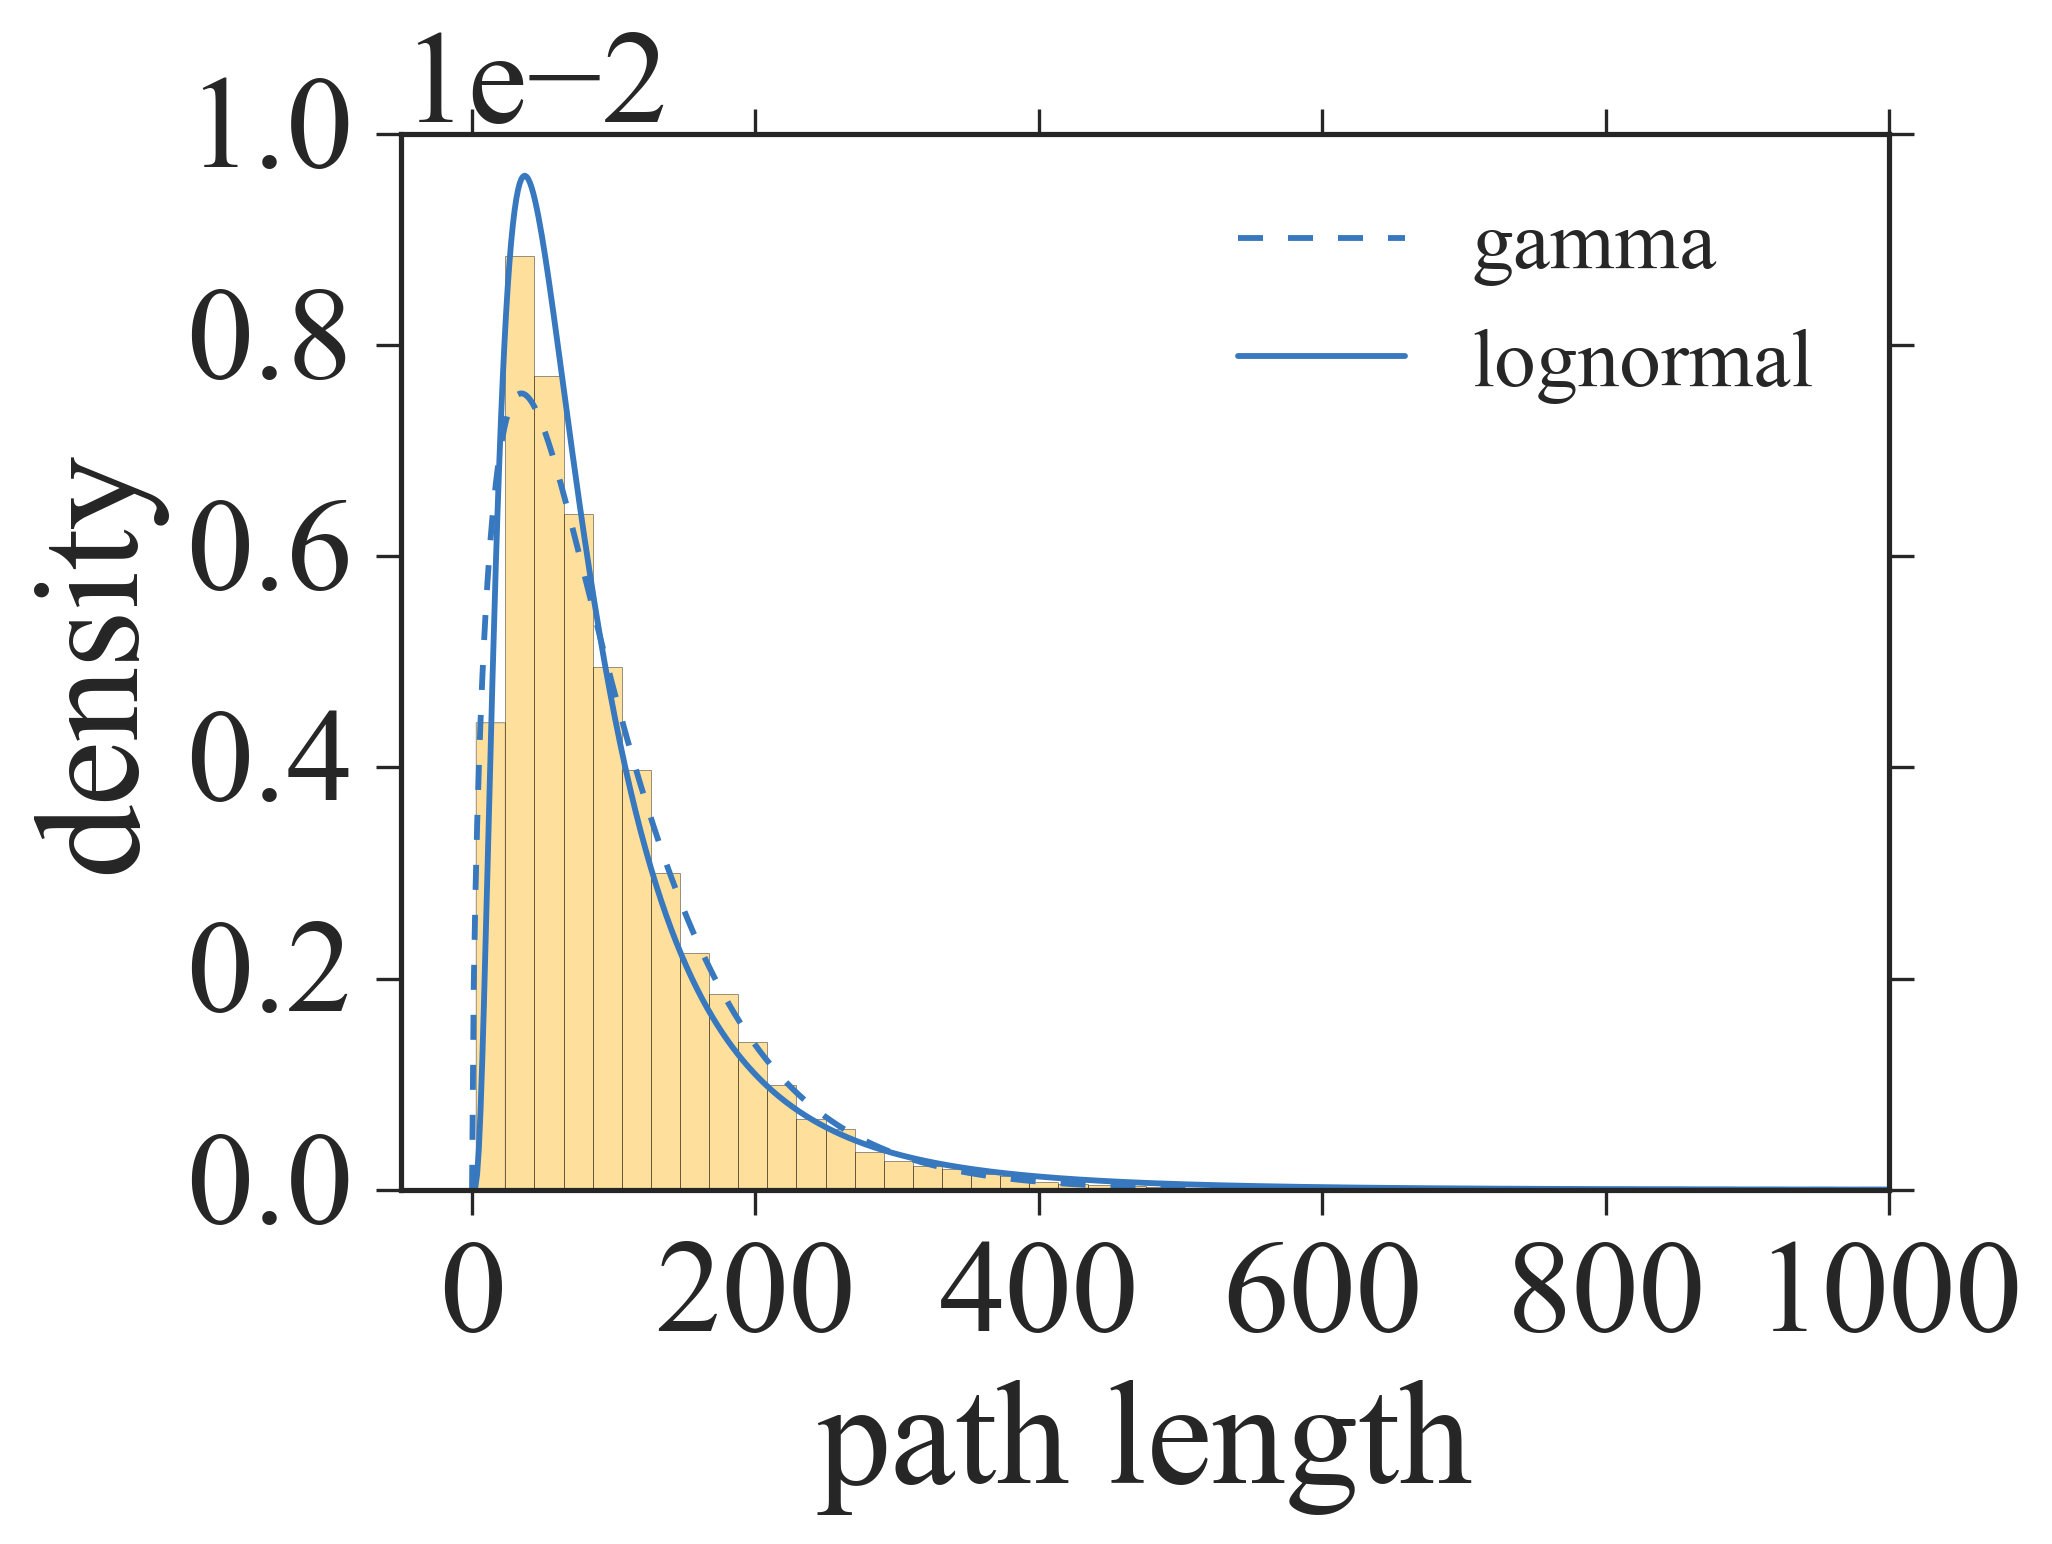
\includegraphics[width=\twoimageswide,keepaspectratio]{path_length/path_length_motion22.png}\qquad
			\label{fig:path_lengths_22}}
			\subfloat[][]{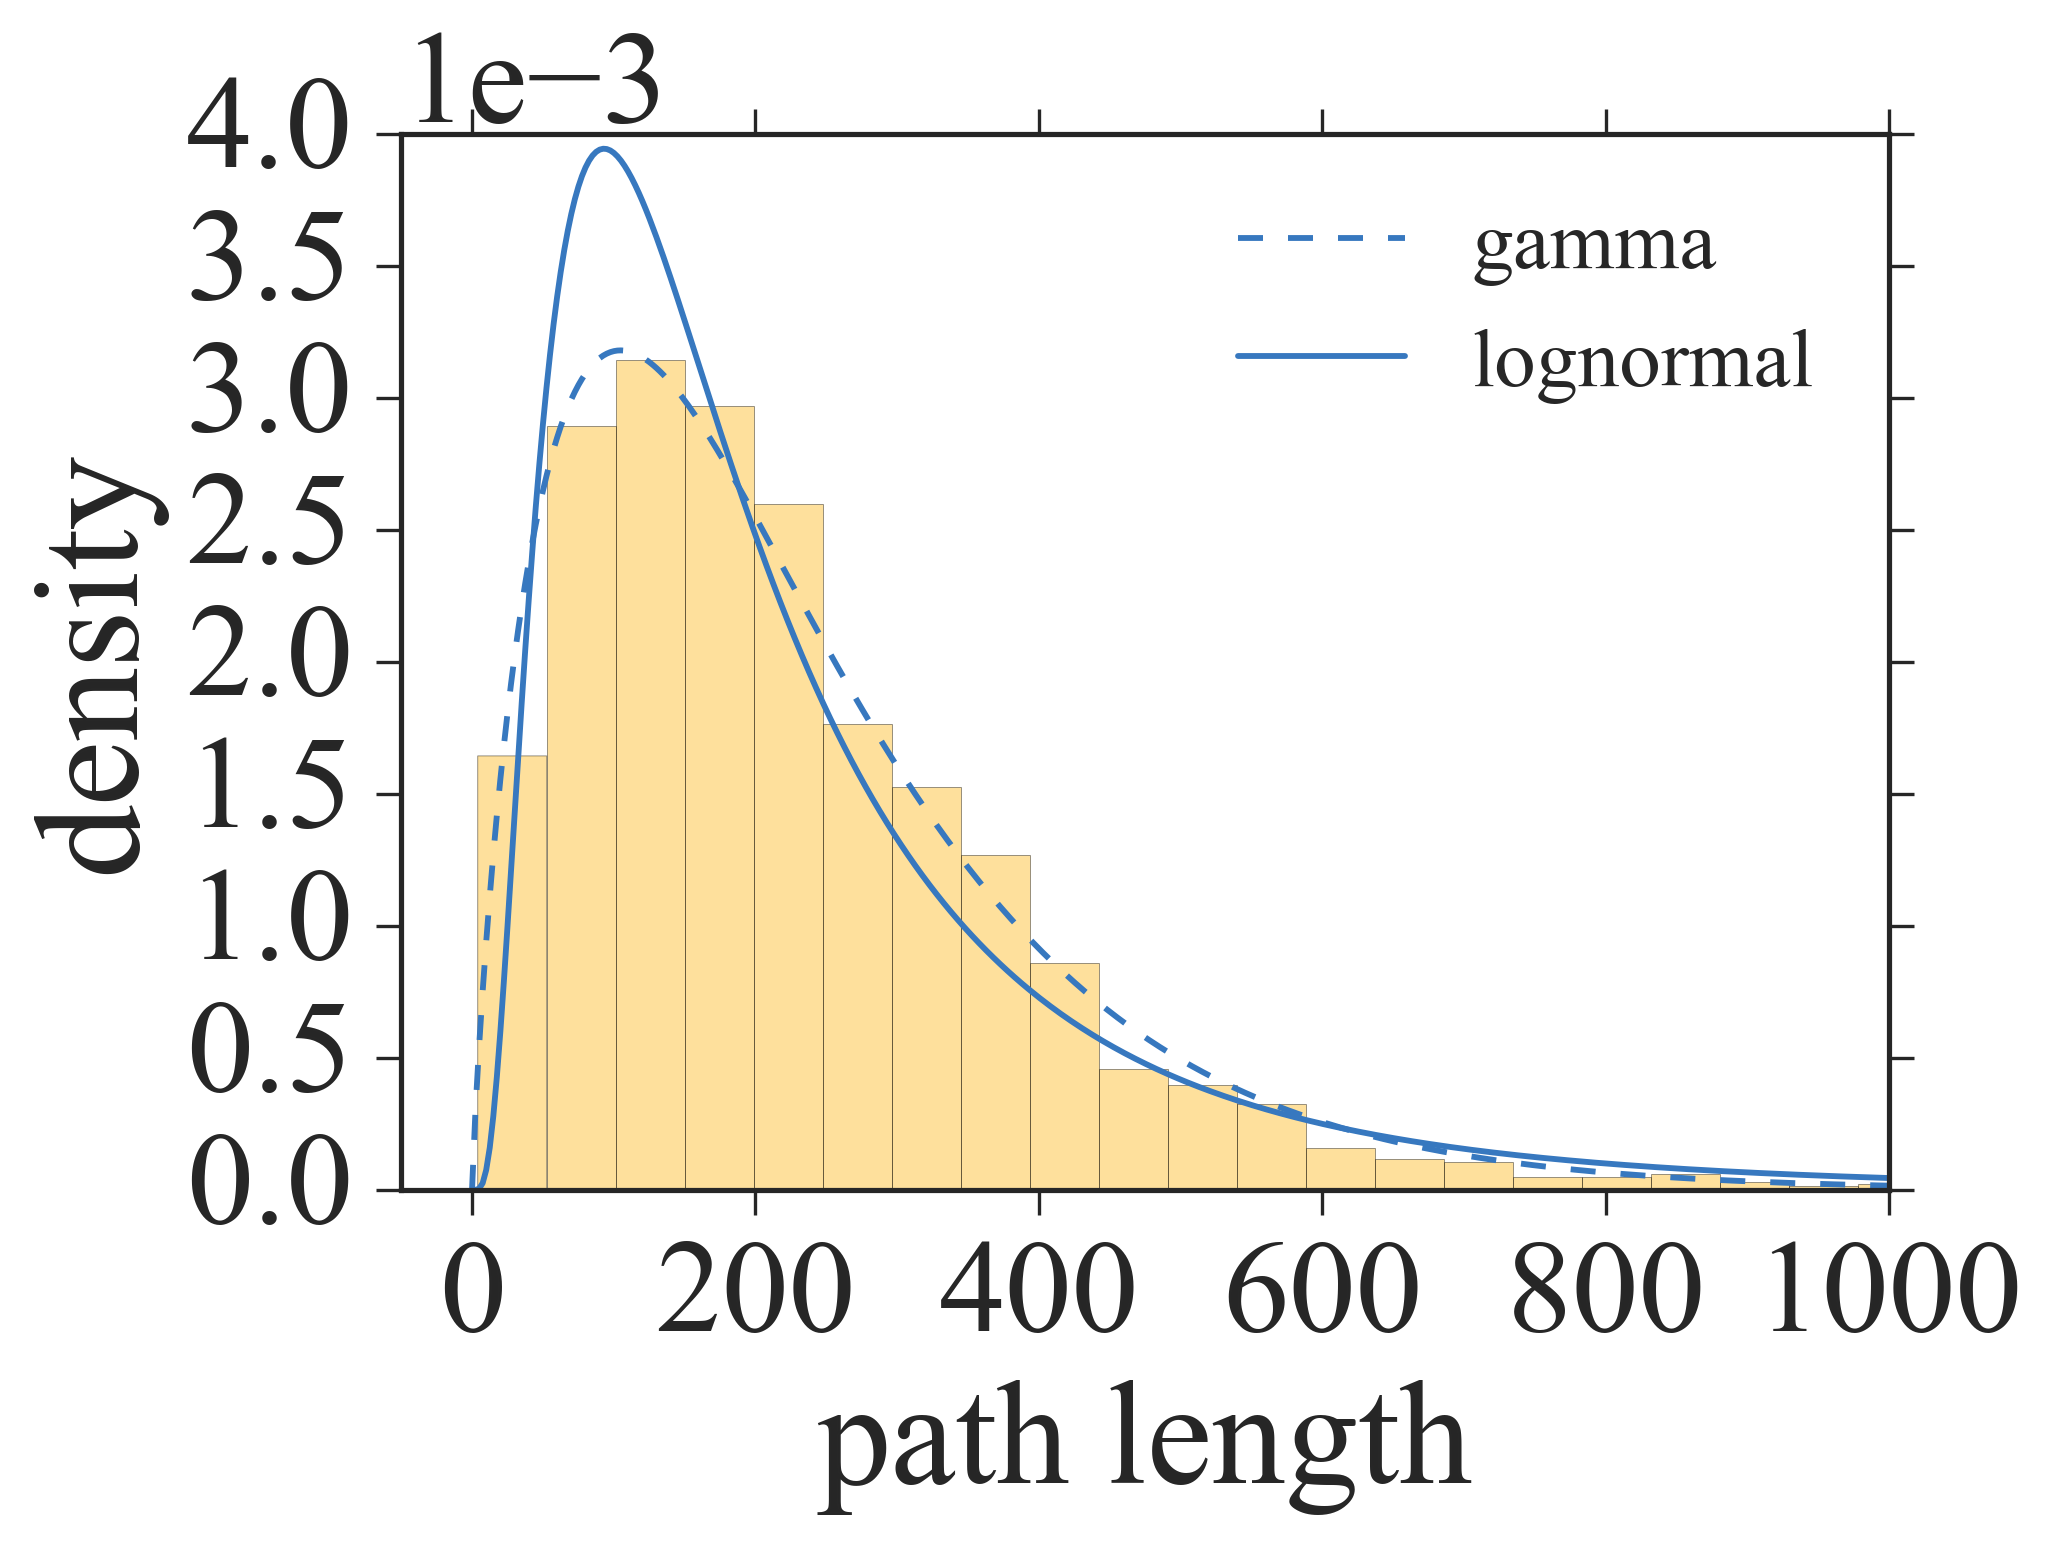
\includegraphics[width=\twoimageswide,keepaspectratio]{path_length/path_length_motion35.png}
			\label{fig:path_lengths_35}}

			\caption[Path length distribution]{Empirical cumulative path length distributions for \series{22} (a) and \series{35} (b). Associated gamma and log-normal fits are shown. Abscissa in units of \si{\pixel}.}
			\label{fig:path_lengths}
		\end{figure}

		We choose the case of \series{22} to illustrate the process we apply to deal with the observed ambiguities in detail. To do so we compare the goodness-of-fit plots associated with fitting a gamma, log-normal distribution and other candidate distributions in \Fref{fig:sup::path_lengths_goodness}. Empirical and theoretical CDFs are in excellent agreement for both gamma and log-normal fits. The same holds true for the P-P plot where empirical and theoretical probabilities coincide, illustrating that both fits do not suffer from ``lack-of-fit'' in the center of the distribution. Looking at the Q-Q plots however, differences between empirical and theoretical quantiles can be seen, indicating that both gamma and log-normal fits are lacking in the right tails of the distributions. The gamma fit could be favored in the end, since it is not as lacking as the log-normal fit when it comes to the right tails, \ie the longer path lengths. We remark that an exponential distribution was attributed to path lengths in previous work~\cite{baumgarten2010plasmodial}. Our data indicates that it is a possible choice, provided a good description of the right tail is desired and the comparatively weak performance in the center of the distribution is not an issue.

		We stress at this point that in order to assess the match between data and fit it is not sufficient to check the agreement between theoretical and empirical distributions alone. Since the latter is given as a density histogram, our perception can easily be mislead by an unfortunate choice of bin sizes. To mitigate this problem we rely on the Freedman–Diaconis rule to determine optimal bin sizes~\cite{freedman1981histogram}. In combination with the goodness-of-fit plots a reliable judgment of fit quality can thus be achieved. 

		The example of \series{22} is illustrative of the difficulties in determining descriptive theoretical distributions we encounter for almost all our data series. Given the available empirical data it is not possible to choose a single distribution from the proposed candidates that captures the tails and the centers equally well for all data series. As a result, depending on what part of the data is of interest one may opt for different theoretical distributions to maximize the usefulness of the description.

		It is our impression however, that the gamma distribution yields a good compromise between center and tail accuracy in most cases. Thus we shall proceed with reporting the properties of the gamma fits in this manuscript. Details of properties of other fit options are available in the complete collection of results. 

		Given a time-ordered data series, one may study the obtained fit parameters as a function of time. For a gamma distribution these are the shape $s$ and the rate $r$ of the distribution. \Fref{fig:path_lengths_fit_parameters} compares the time development of the parameters obtained for two long-running data series. Despite the considerable fluctuations, it can be seen in \Fref{fig:path_lengths_fit_parameters_shape} that the shape has a tendency to increase, while the rate is slightly declining as shown in \Fref{fig:path_lengths_fit_parameters_rate}. Since the mode of the gamma distribution is given by $(s-1)/r$ for $s > 1$, its value is increasing with time for both data series. It follows that the most likely path length to be observed increases in value as time moves on. This is accompanied by a shift of probability mass towards longer paths, which is consistent with network coarsening. 

		\begin{figure}
			\centering
			\subfloat[][]{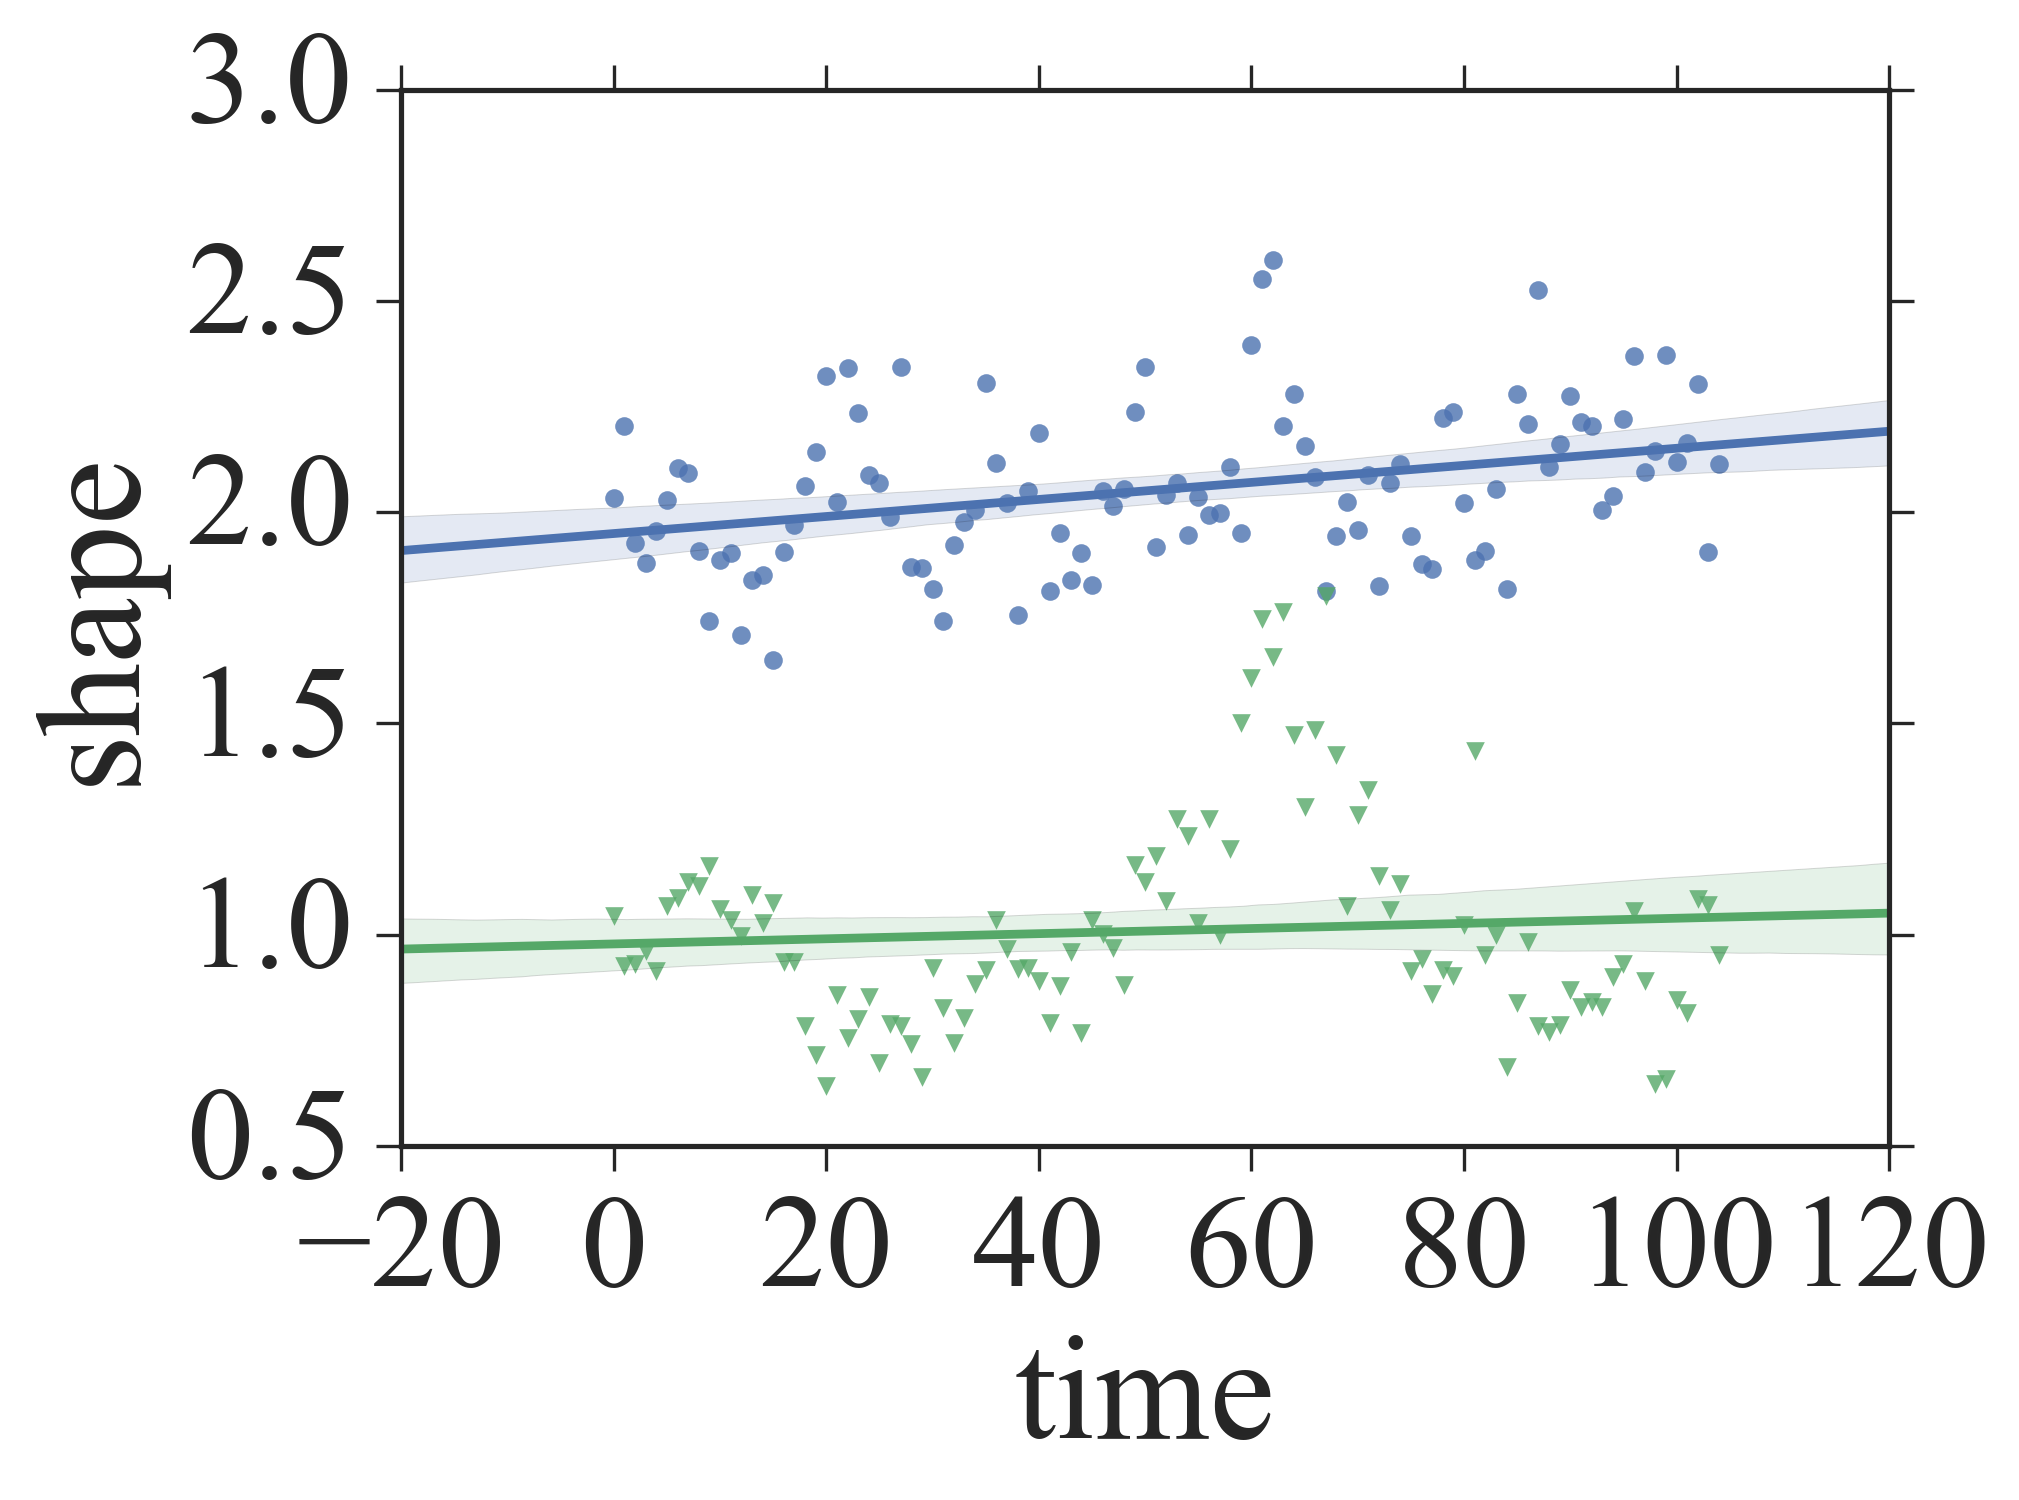
\includegraphics[width=\twoimageswide,keepaspectratio]{path_length/physical_edge_length_gamma_fit_shape_35_58.png}
			\label{fig:path_lengths_fit_parameters_shape}}\qquad
			\subfloat[][]{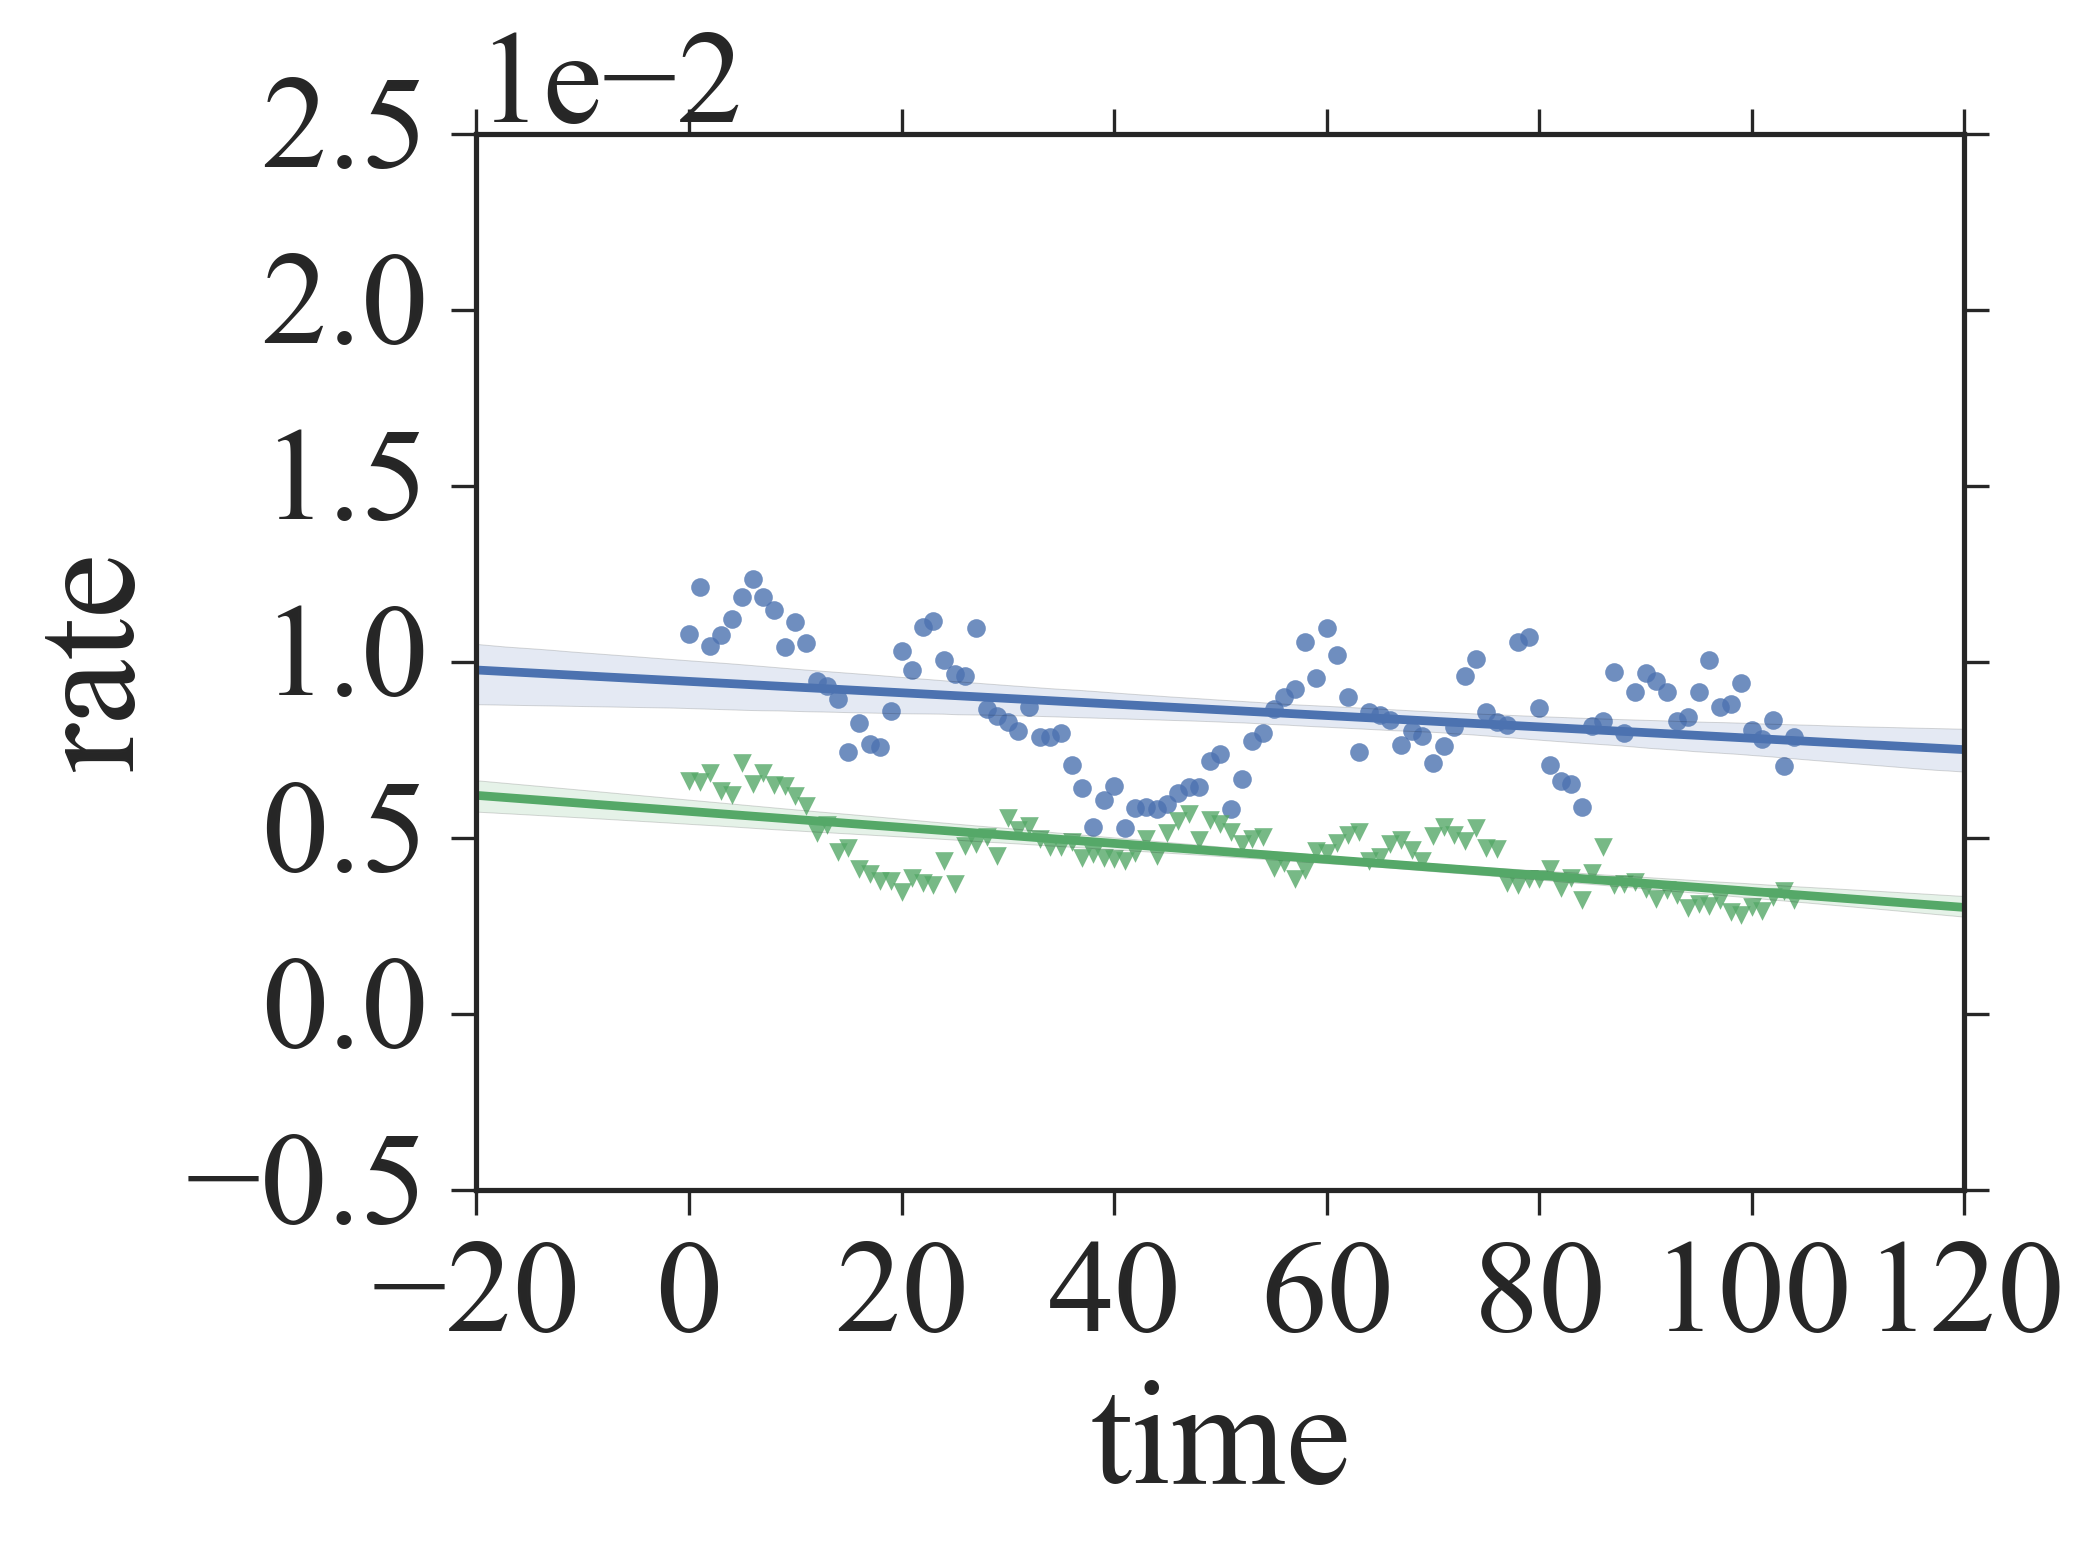
\includegraphics[width=\twoimageswide,keepaspectratio]{path_length/physical_edge_length_gamma_fit_rate_35_58.png}
			\label{fig:path_lengths_fit_parameters_rate}}

			\caption[Path length distribution - Fit parameters]{Time dependence of shape $s$ (a) and rate $r$ (b) for \series{35} (blue circles) and \series{58} (green triangles). Linear fits are shown to guide the eye. Abscissa in units of \SI{120}{\second}.}
			\label{fig:path_lengths_fit_parameters}
		\end{figure}

		I addition to the time development of the fit parameters within distinct data series, we investigate the obtained values across the entire data set that has been fit. \Fref{fig:path_lengths_gamma_fit_kde} shows the scatter-plot of $s$ and $r$ and the associated estimated kernel density. The result illustrates what characteristic ranges of fit parameters, and by extension distributions, one may expect to encounter when it comes to path lengths in \P graphs. Given the location of the density maximum, we can compute the mode of the associated gamma distribution and obtain \SI{107.2389}{\pixel}.

		\begin{figure}[!htbp]
			\centering
				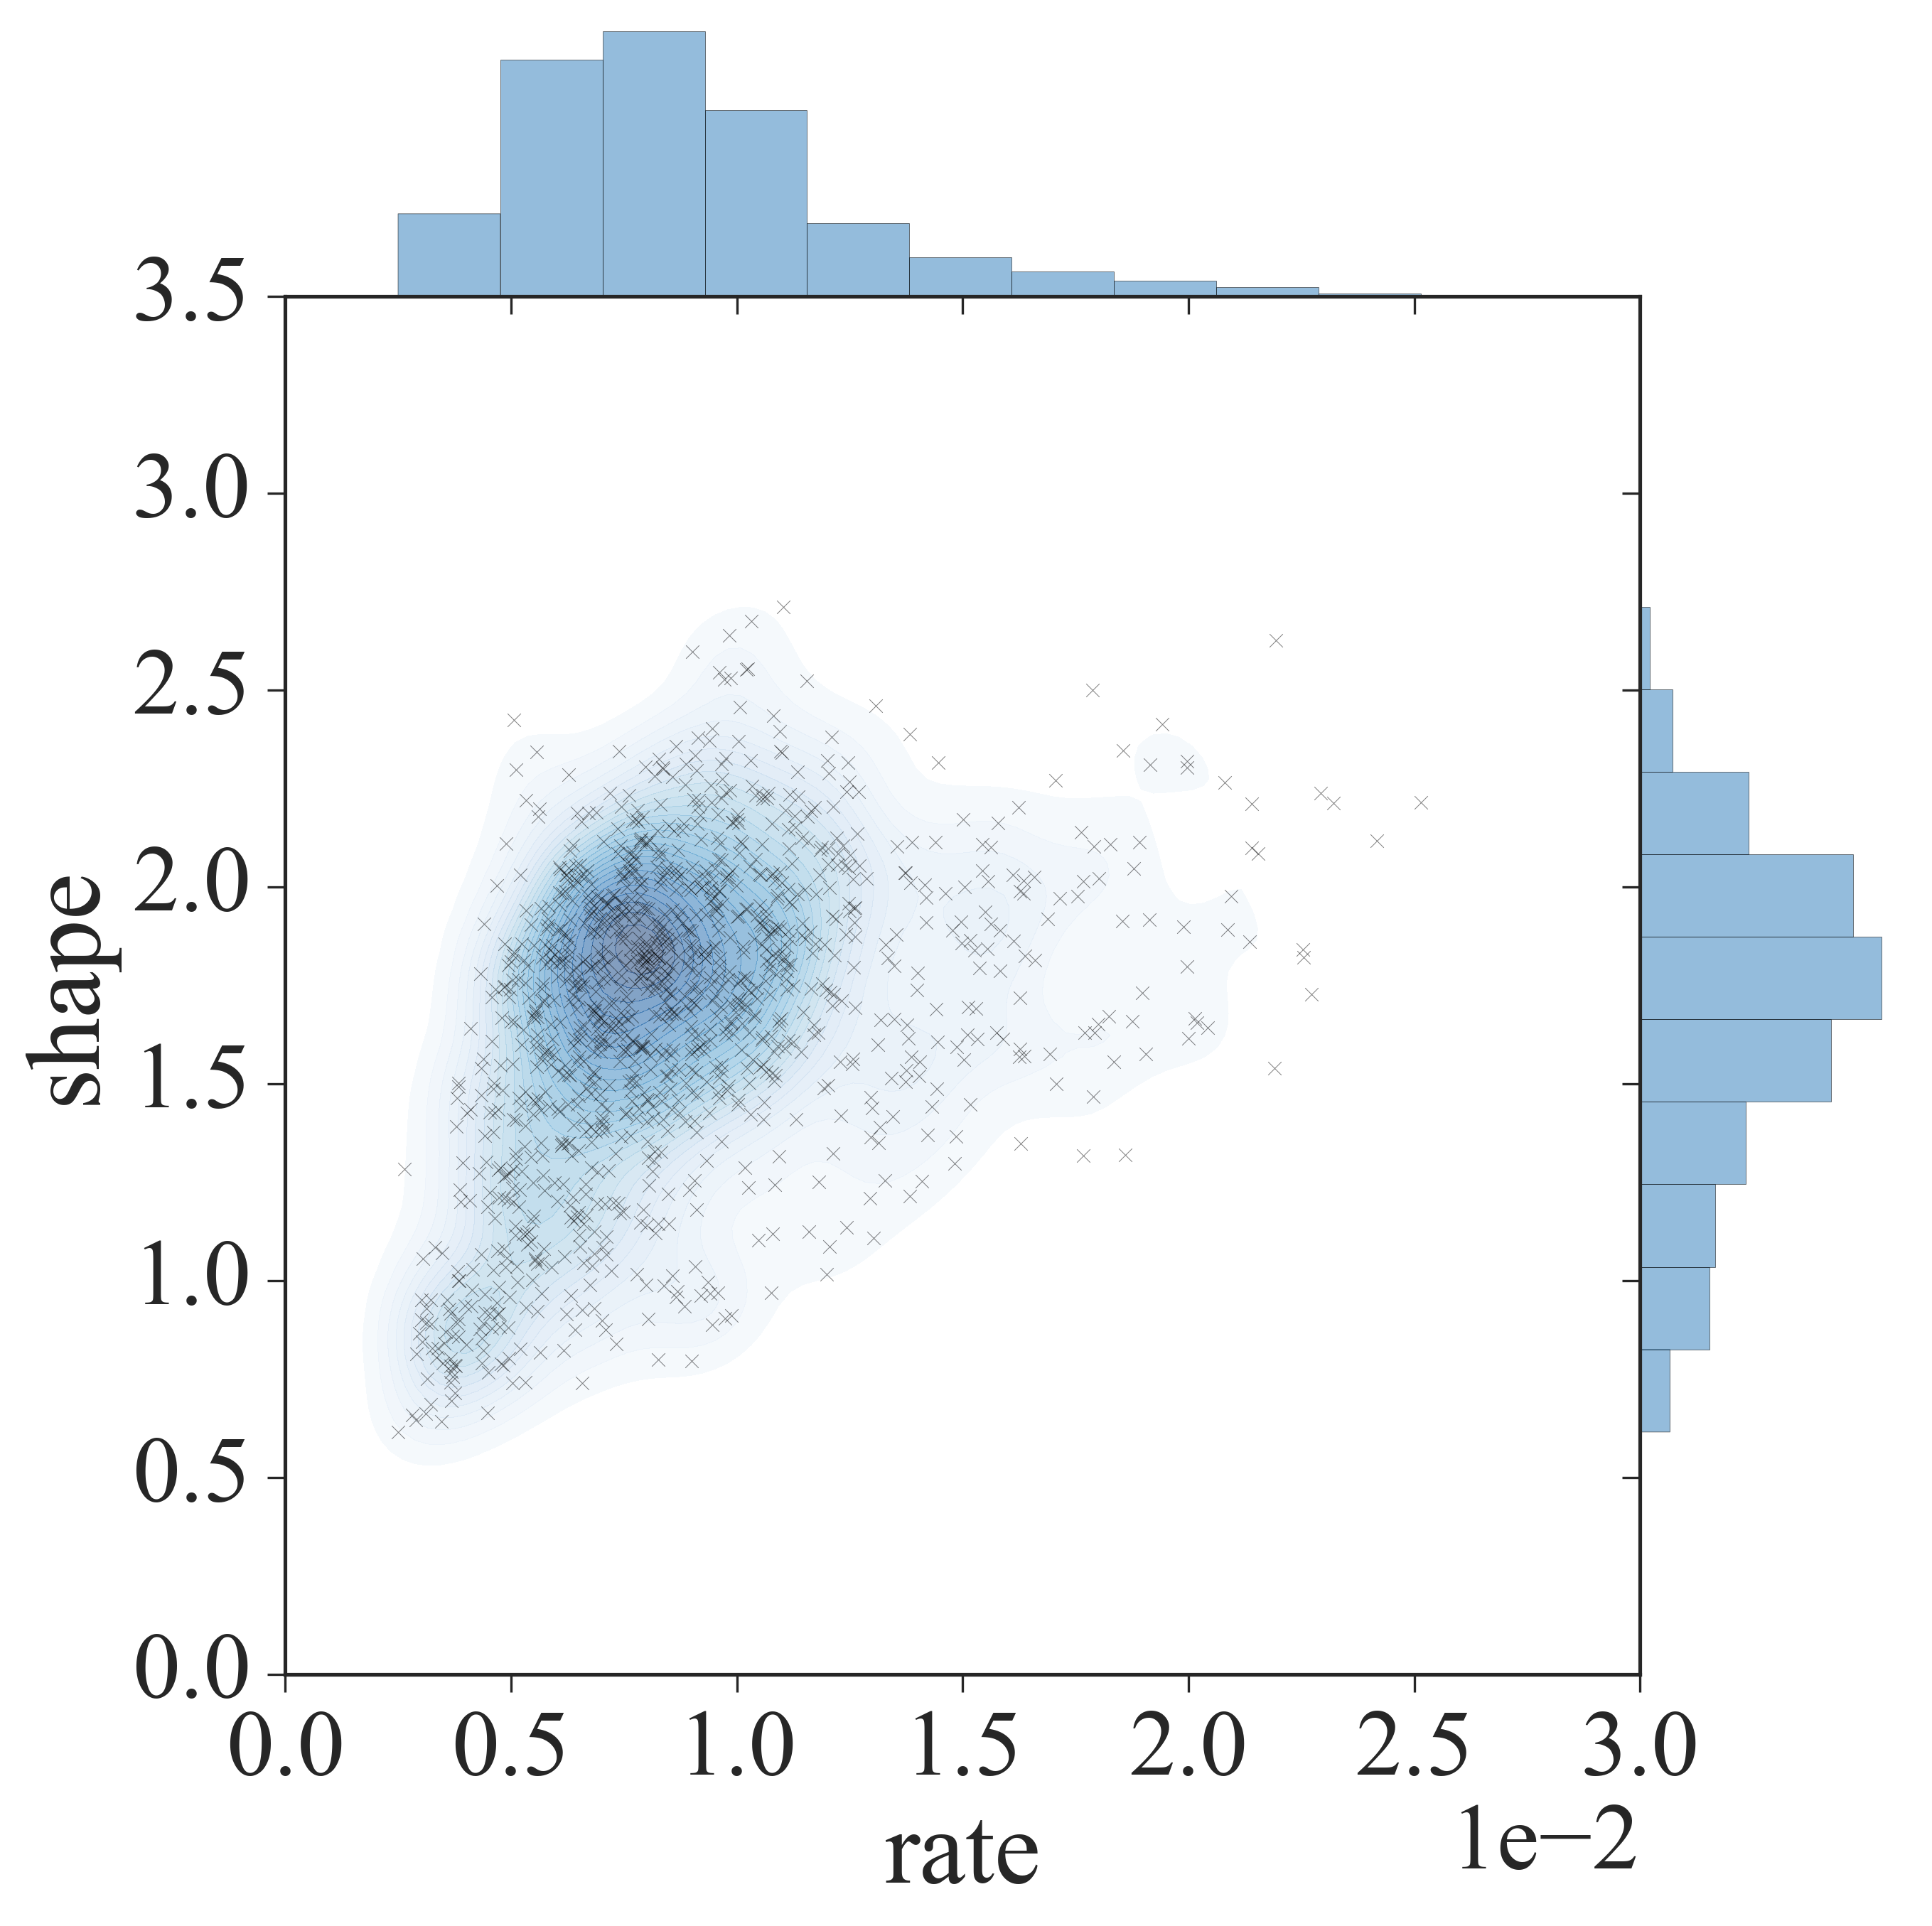
\includegraphics[width=0.75\textwidth]{path_length/physical_edge_length_gamma_fit_rate_shape_scatter_cummulative.png}
			\caption[Path length distribution - Fit parameter densities]{Scatter-plot and kernel density estimates of shape $s$ and rate $r$ for gamma fits of empirical path lengths using the entire dataset. The maximum of the density is located at $s = 1.8403$ and $r \approx 0.7836 \times 10^{-2}$.}
			\label{fig:path_lengths_gamma_fit_kde}
		\end{figure}

		After detailing the procedure applied to the path lengths we proceed by investigating the average path widths and the path volume in the same manner. Since the procedure is the same, we keep the description more concise from now on.

		Let us define the average path width as the average over the individual edge widths a path contains. In \Fref{fig:path_widths} we compare the empirical path width distributions of \series{22} and \series{35}. Yet again an inspection of the density histograms alone does not allow to decide between the two most promising candidate distributions and we look to the goodness-of-fit plots to learn more. \Fref{fig:sup::path_widths_goodness} shows that for \series{35}, both gamma and log-normal fits do not suffer from lack-of-fit in the tails of the distribution. Furthermore, empirical and theoretical CDFs agree. At the same time, the P-P plot indicates that both options are lacking in the center of the distribution. Both gamma and log-normal fits yield almost the same fit quality, even a normal fit yields a usable description. In the end, we favor the gamma fit yet again, because it delivers slightly better Q-Q plots. 

		\begin{figure}
			\centering
			\subfloat[][]{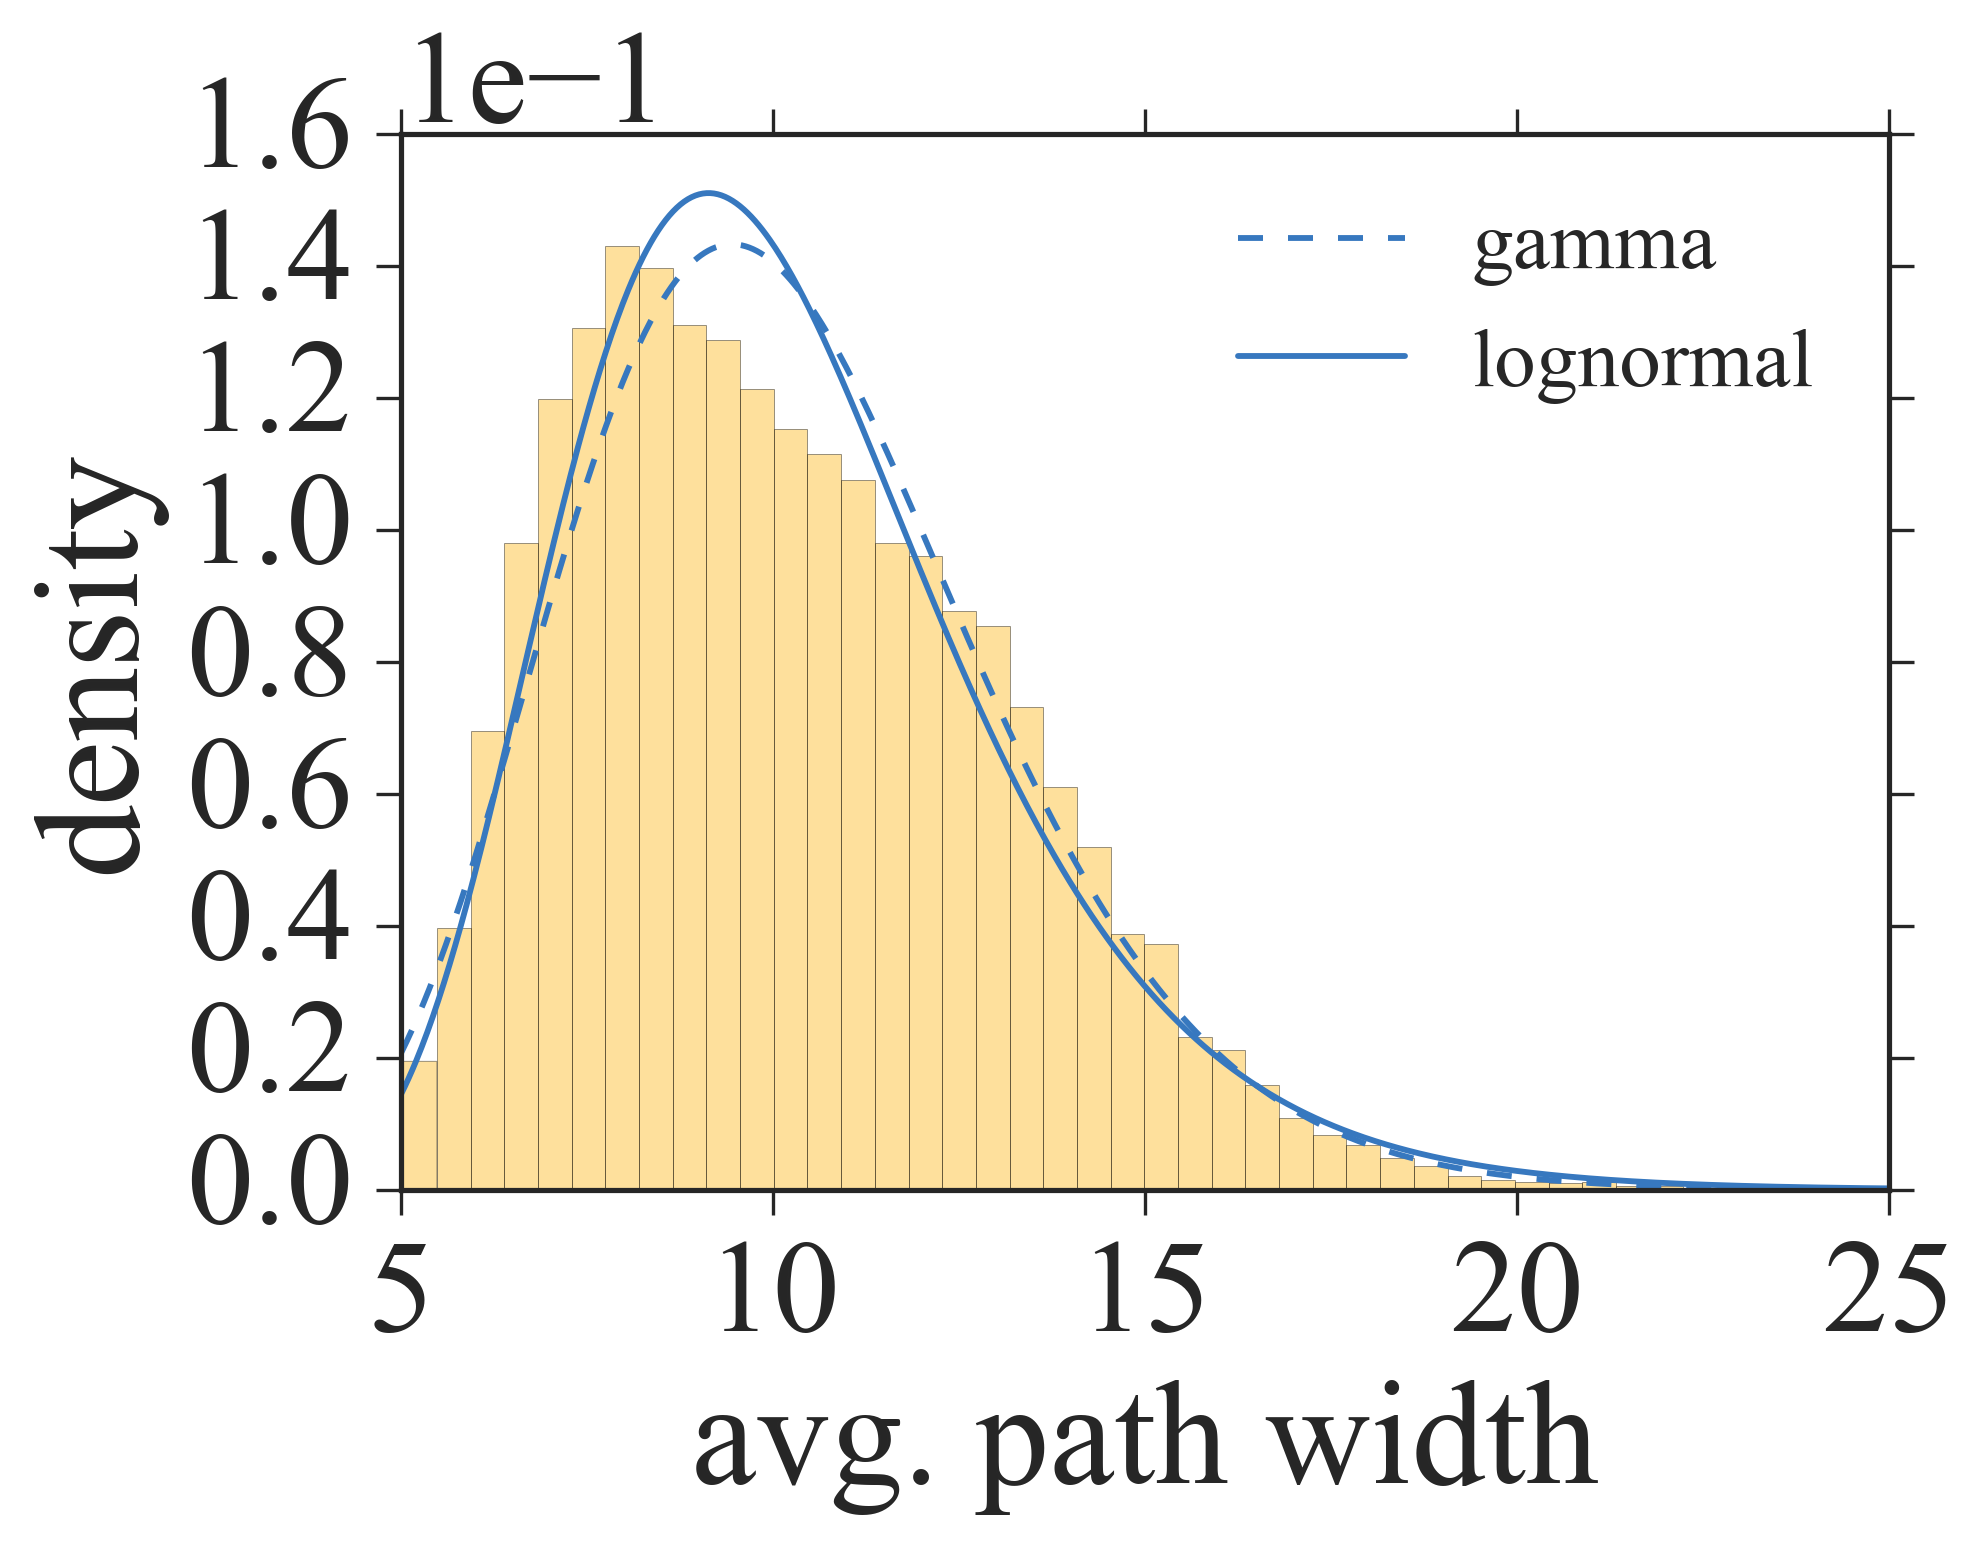
\includegraphics[width=\twoimageswide,keepaspectratio]{path_width/path_width_motion22.png}
			\label{fig:path_widths_22}}\qquad
			\subfloat[][]{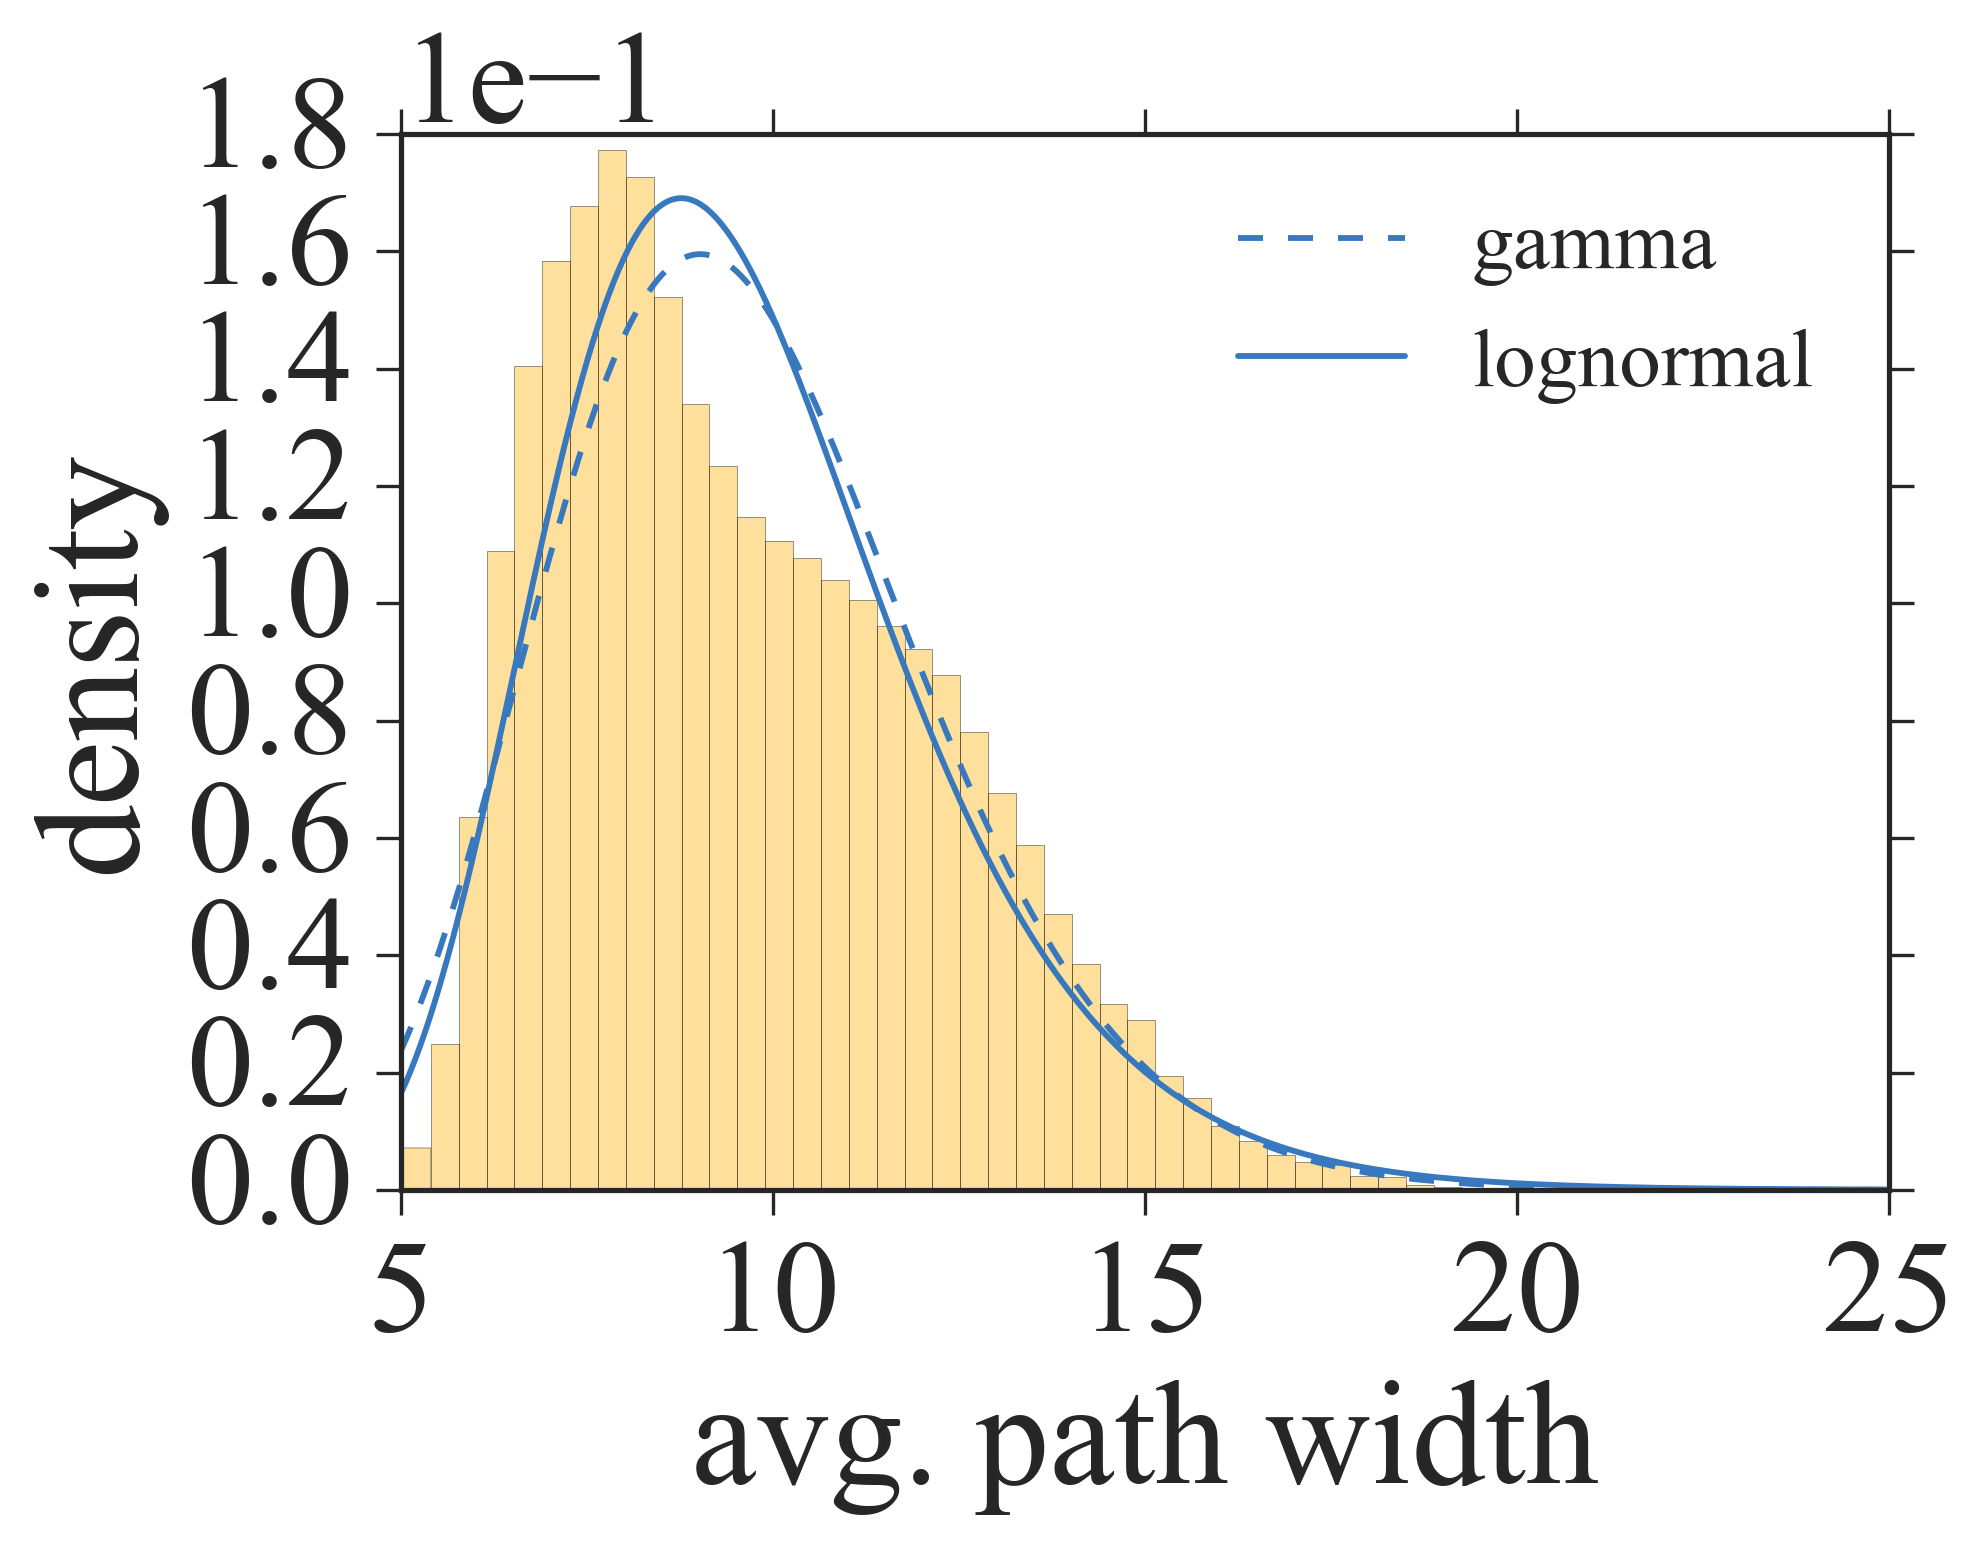
\includegraphics[width=\twoimageswide,keepaspectratio]{path_width/path_width_motion35.png}
			\label{fig:path_widths_35}}

			\caption[Path width distribution]{Empirical cumulative distributions of average path widths for \series{22} (a) and \series{35} (b). Associated gamma and log-normal fits are shown. Abscissa in units of \si{\pixel}.}
			\label{fig:path_widths}
		\end{figure}

		Taking into account the whole data set, the theoretical distribution of the average paths widths remains undecidable. The differences between gamma and log-normal fits are minute and thus the fact that earlier work attested a log-normal behavior of the widths is still supported by our findings~\cite{baumgarten2010plasmodial}. We remark that, the pronounced ``shoulder'' seen in \Fref{fig:path_widths_35} suggest to the eye that a bimodal distribution could be responsible for the observations. Thus we attempted to fit the path widths with a Gaussian mixture. However, we failed to satisfy the associated statistical tests conforming that a Gaussian mixture is indeed the correct underlying distribution.

		Next we report the gamma fit parameters as a function of time. \Fref{fig:path_width_fit_parameters} compares the time development of the parameters obtained for \series{35} and \series{58}. Note that, for both series a linear relationship between shape $s$ and rate $r$ can be observed. For \series{35} we find that $s(r) = (\num{8.0634 \pm 0.116}) r + (\num{2.4148 \pm 1.841})$ holds. At the same time we obtain $s(r) = (\num{9.1390 \pm 0.142}) r + (\num{0.5859 \pm 0.187})$ for \series{58}.
		
		\begin{figure}
			\centering
			\subfloat[][]{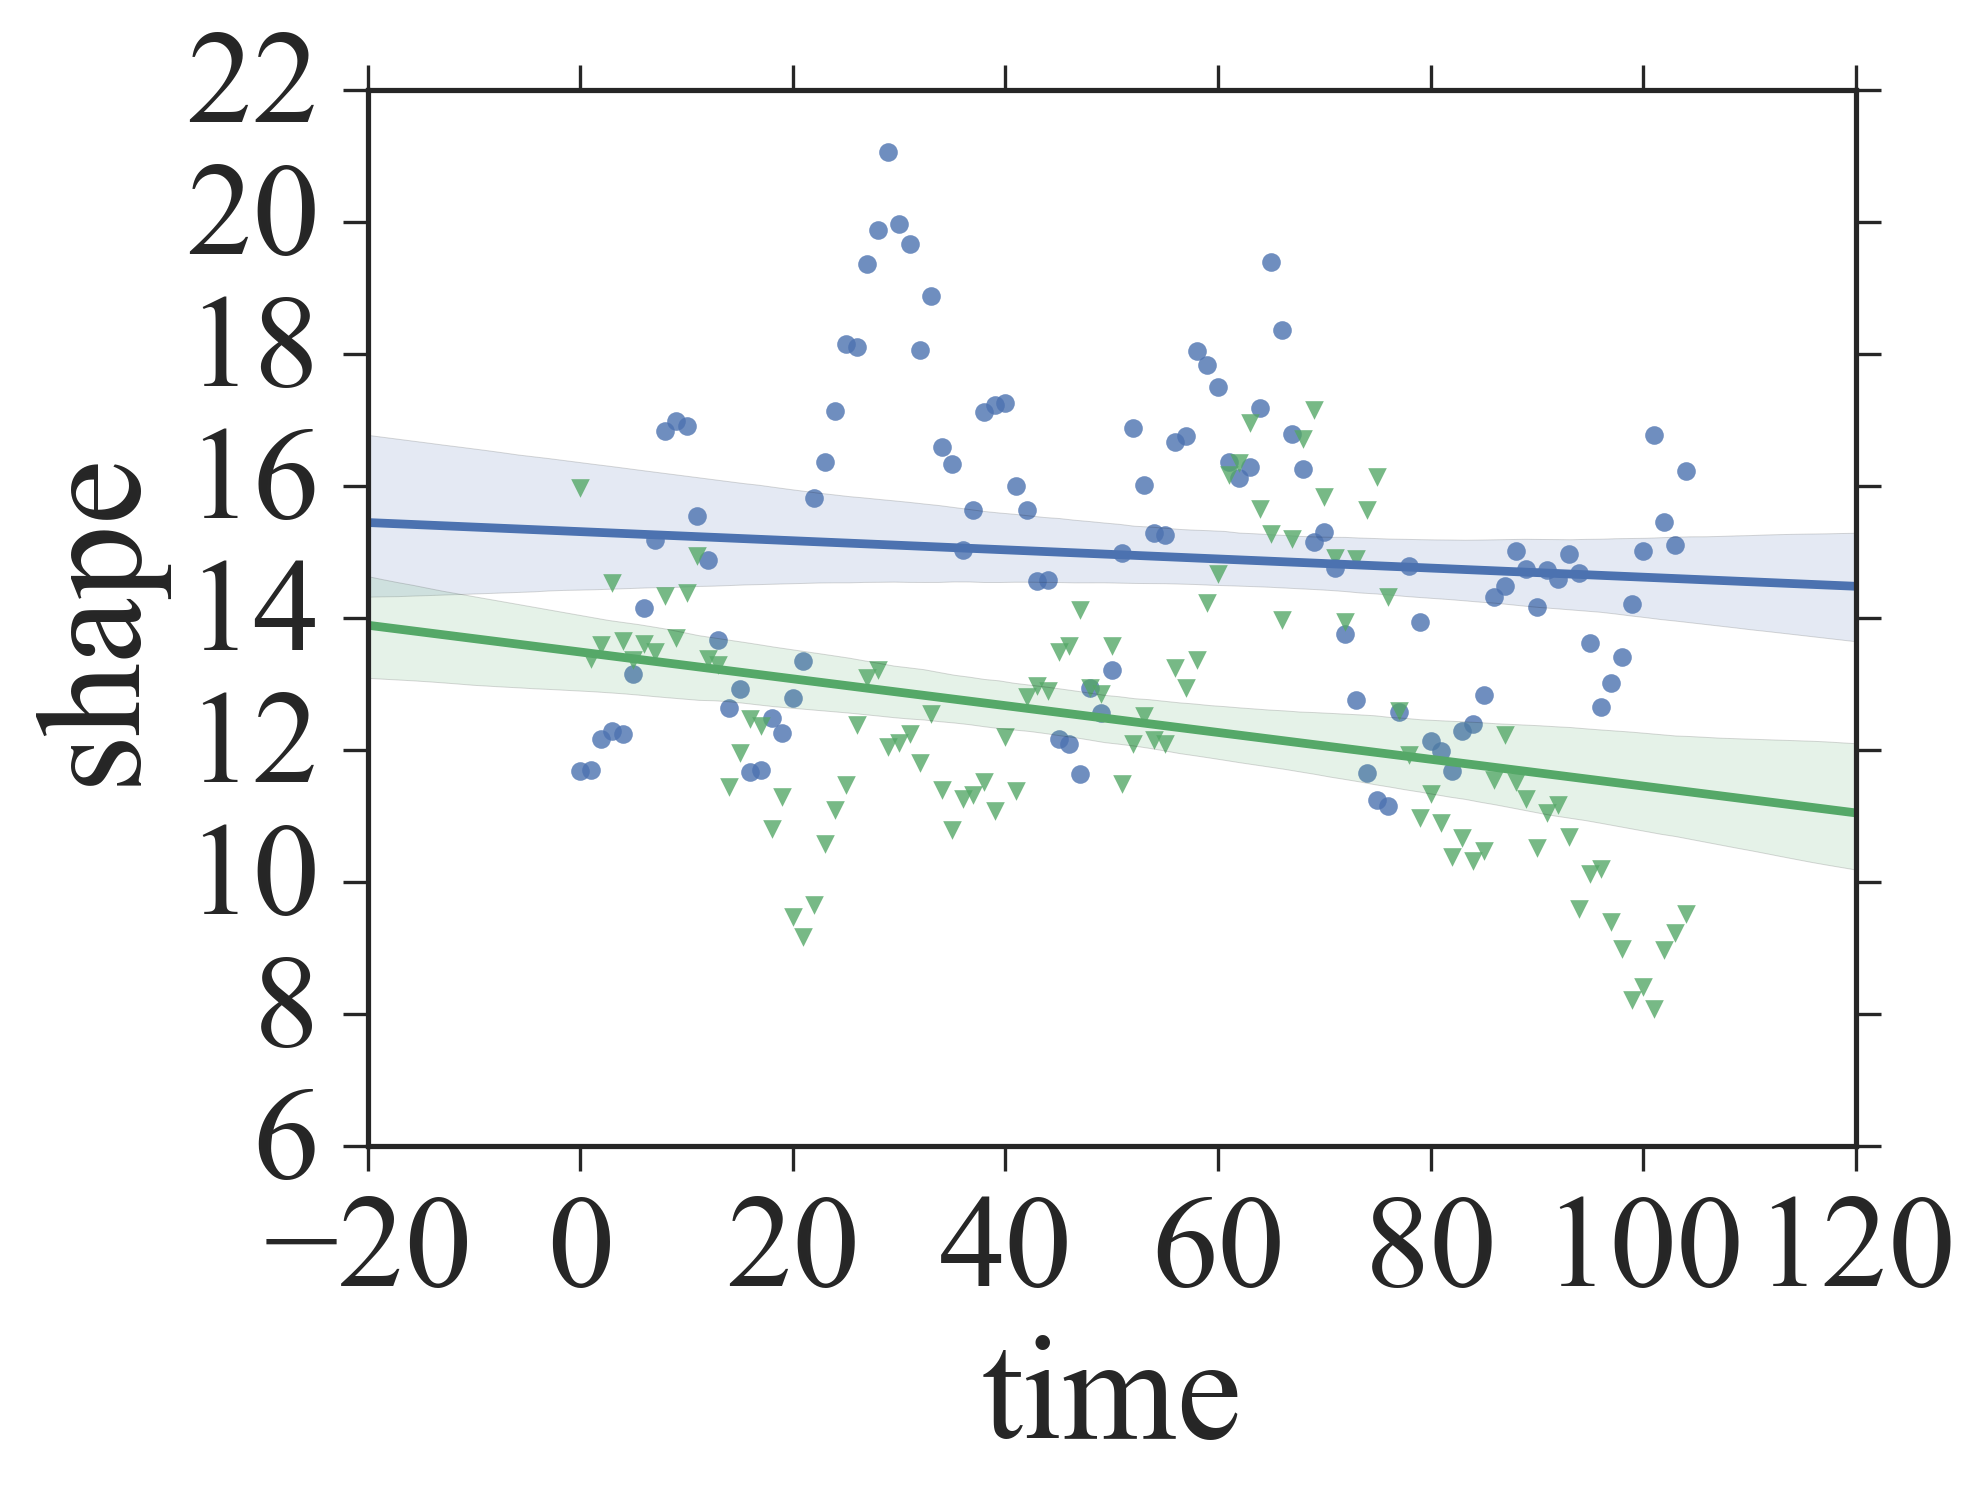
\includegraphics[width=\twoimageswide,keepaspectratio]{path_width/physical_edge_width_gamma_fit_shape_38_58.png}
			\label{fig:path_width_fit_parameters_shape}}\qquad
			\subfloat[][]{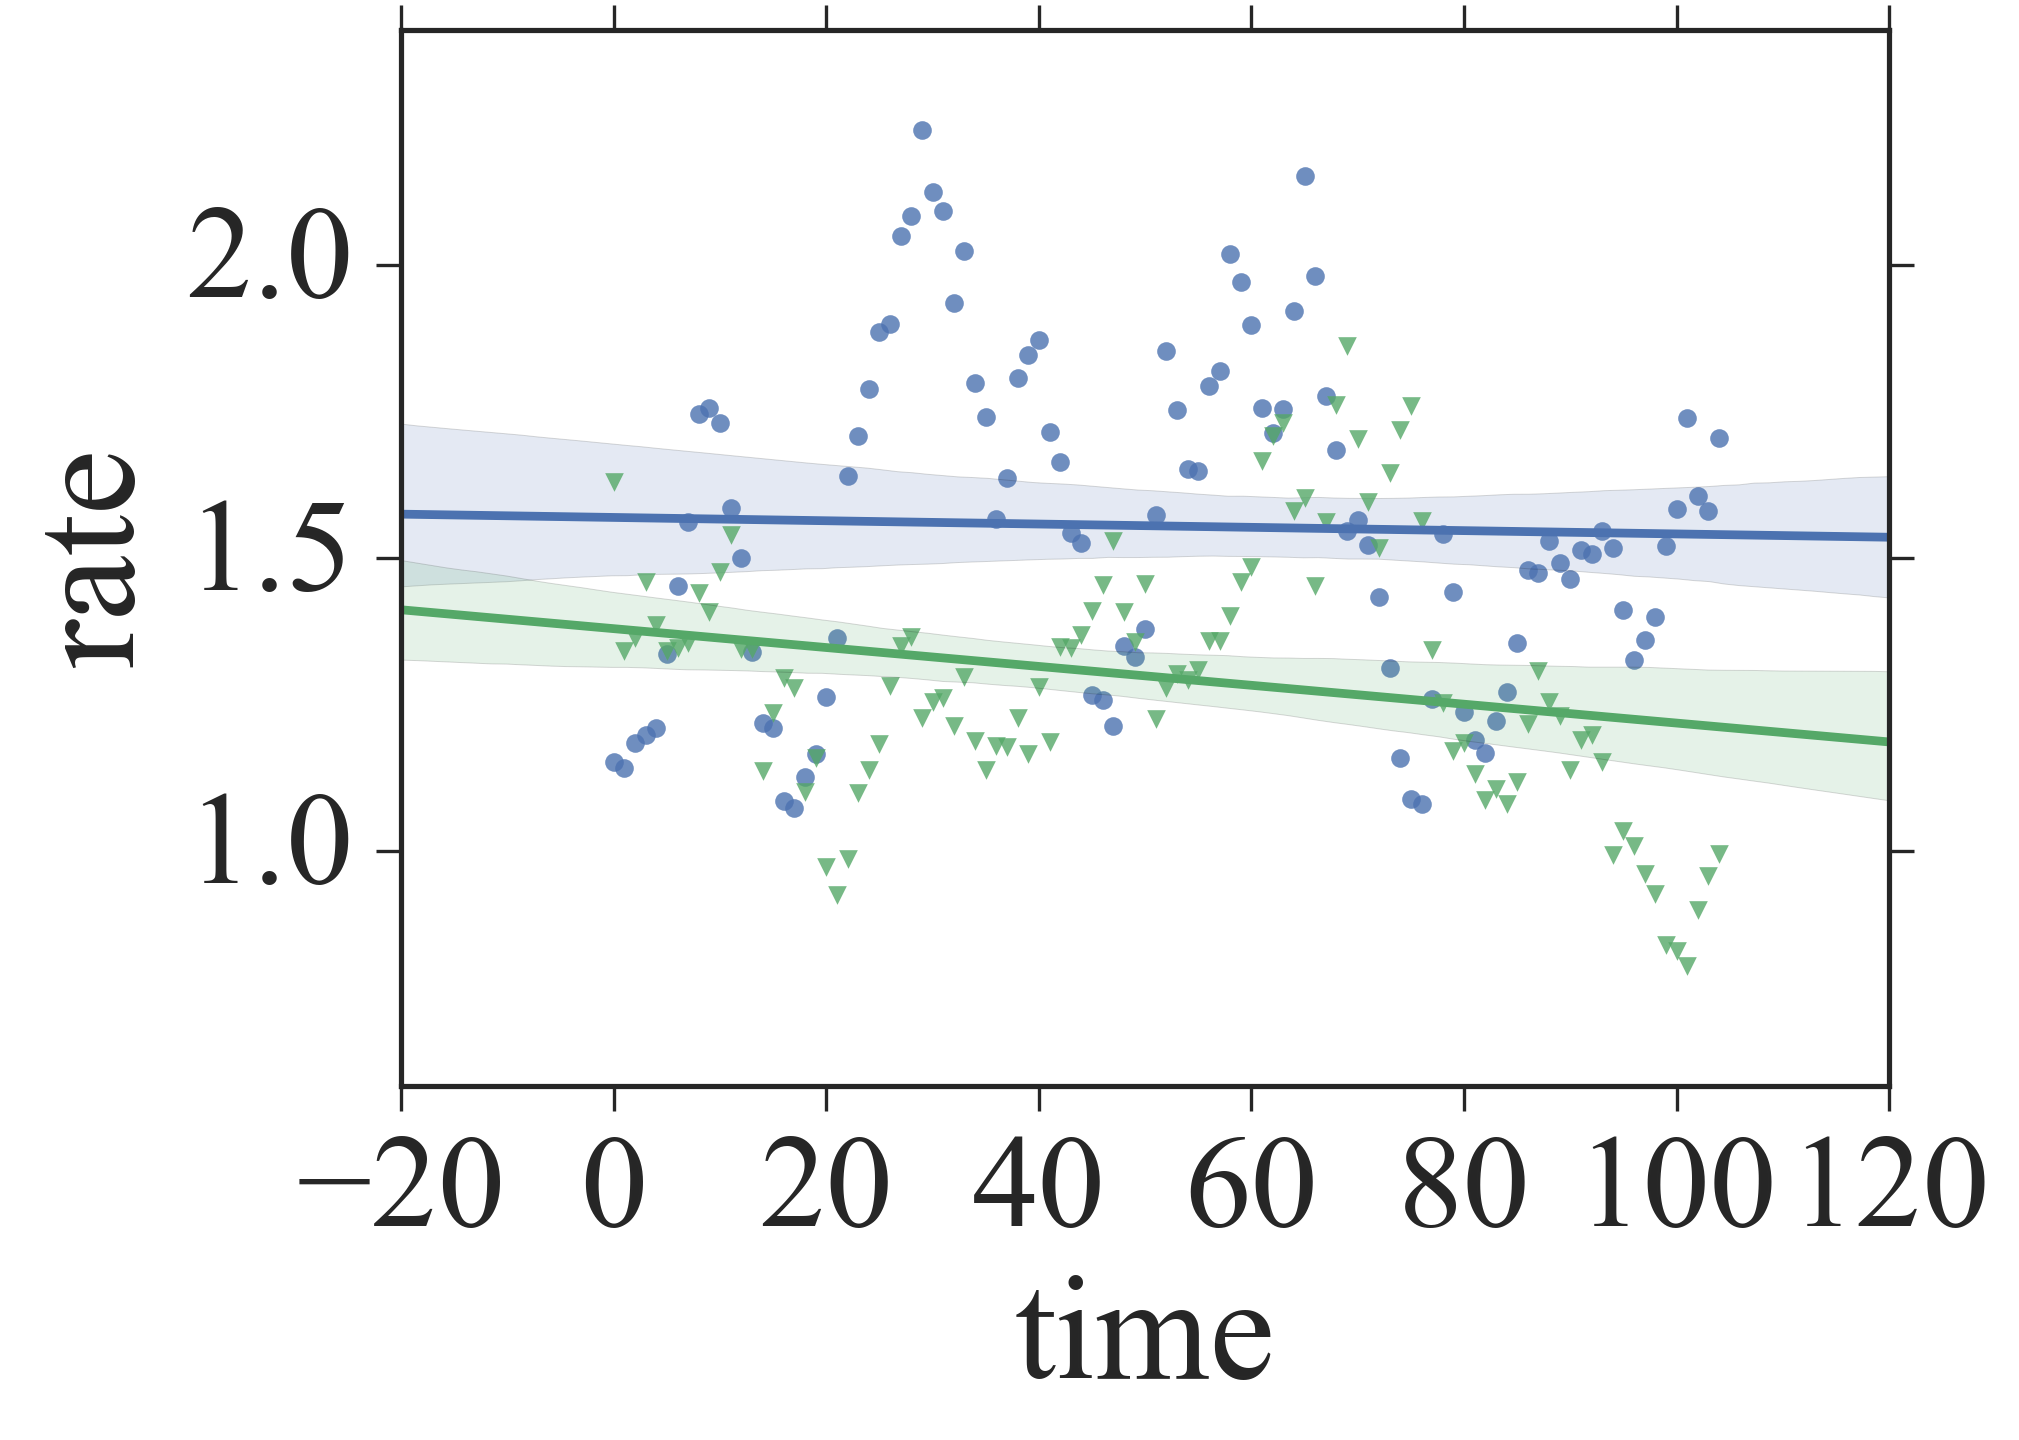
\includegraphics[width=\twoimageswide,keepaspectratio]{path_width/physical_edge_width_gamma_fit_rate_38_58.png}
			\label{fig:path_width_fit_parameters_rate}}

			\caption[Path width distribution - Fit parameters]{Time dependence of shape $s$ (a) and rate $r$ (b) for \series{35} (blue circles) and \series{58} (green triangles). Linear fits are shown to guide the eye. Abscissa in units of \SI{120}{\second}.}
			\label{fig:path_width_fit_parameters}
		\end{figure}


		\Fref{fig:path_widths_gamma_fit_kde} illustrates that a similar linear relation holds across all the available data. It is given by $s(r) = (\num{8.3761 \pm 0.040})\: r + (\num{2.0081 \pm 0.064})$. We believe that this relation follows naturally from the fact that the path widths are relatively small in value and their distributions show only little variation from one data series to the next. In this regards the path widths behave decisively different from the path lengths, which show much larger variation.

		We may use the given linear relation to parametrize the gamma distributions as a function of $r$ and study the effect on the mode and the tails of the distribution as $r$ assumes values in $[0.5,3]$. We find that the position of the mode is confined within a relatively small interval of $[8.467,10.893]$. Furthermore, as $r$ increases the probability mass concentrates around the mode as it is traversing the given interval. At the same time $s(r)$ increases, causing the gamma distribution to approach a normal distribution with $\mu = s/r$ and $\sigma^2= s/r^2$. Thus the distribution of average path widths smoothly interpolates between a gamma distribution for small $r$ and normal distribution for larger $r$. For $r = 1.2799$, which is associated with a maximum in the density plot of \Fref{fig:path_widths_gamma_fit_kde}, the mode takes a value of \SI{9.1637}{\pixel}. The fact that the gamma distribution naturally captures the transition to a normal distributions increases our confidence that the gamma distribution yields a correct description of the data.

		We point out that within the observed range of fit parameters, the probability mass in the right tail of the distribution is largest for small values of $r$. Thus one would expect the rate to drop as time goes by if larger path widths are to become more probable as the slime mold networks undergo coarsening. Looking at \Fref{fig:path_width_fit_parameters}, \series{58} does exhibit this behavior. At the same time \series{35} does not seem to show any long term changes in the rate, which would indicate that the distribution remains stable. Taking into account the entire data set, we repeatedly find both types of behavior.

		\begin{figure}[!htbp]
			\centering
				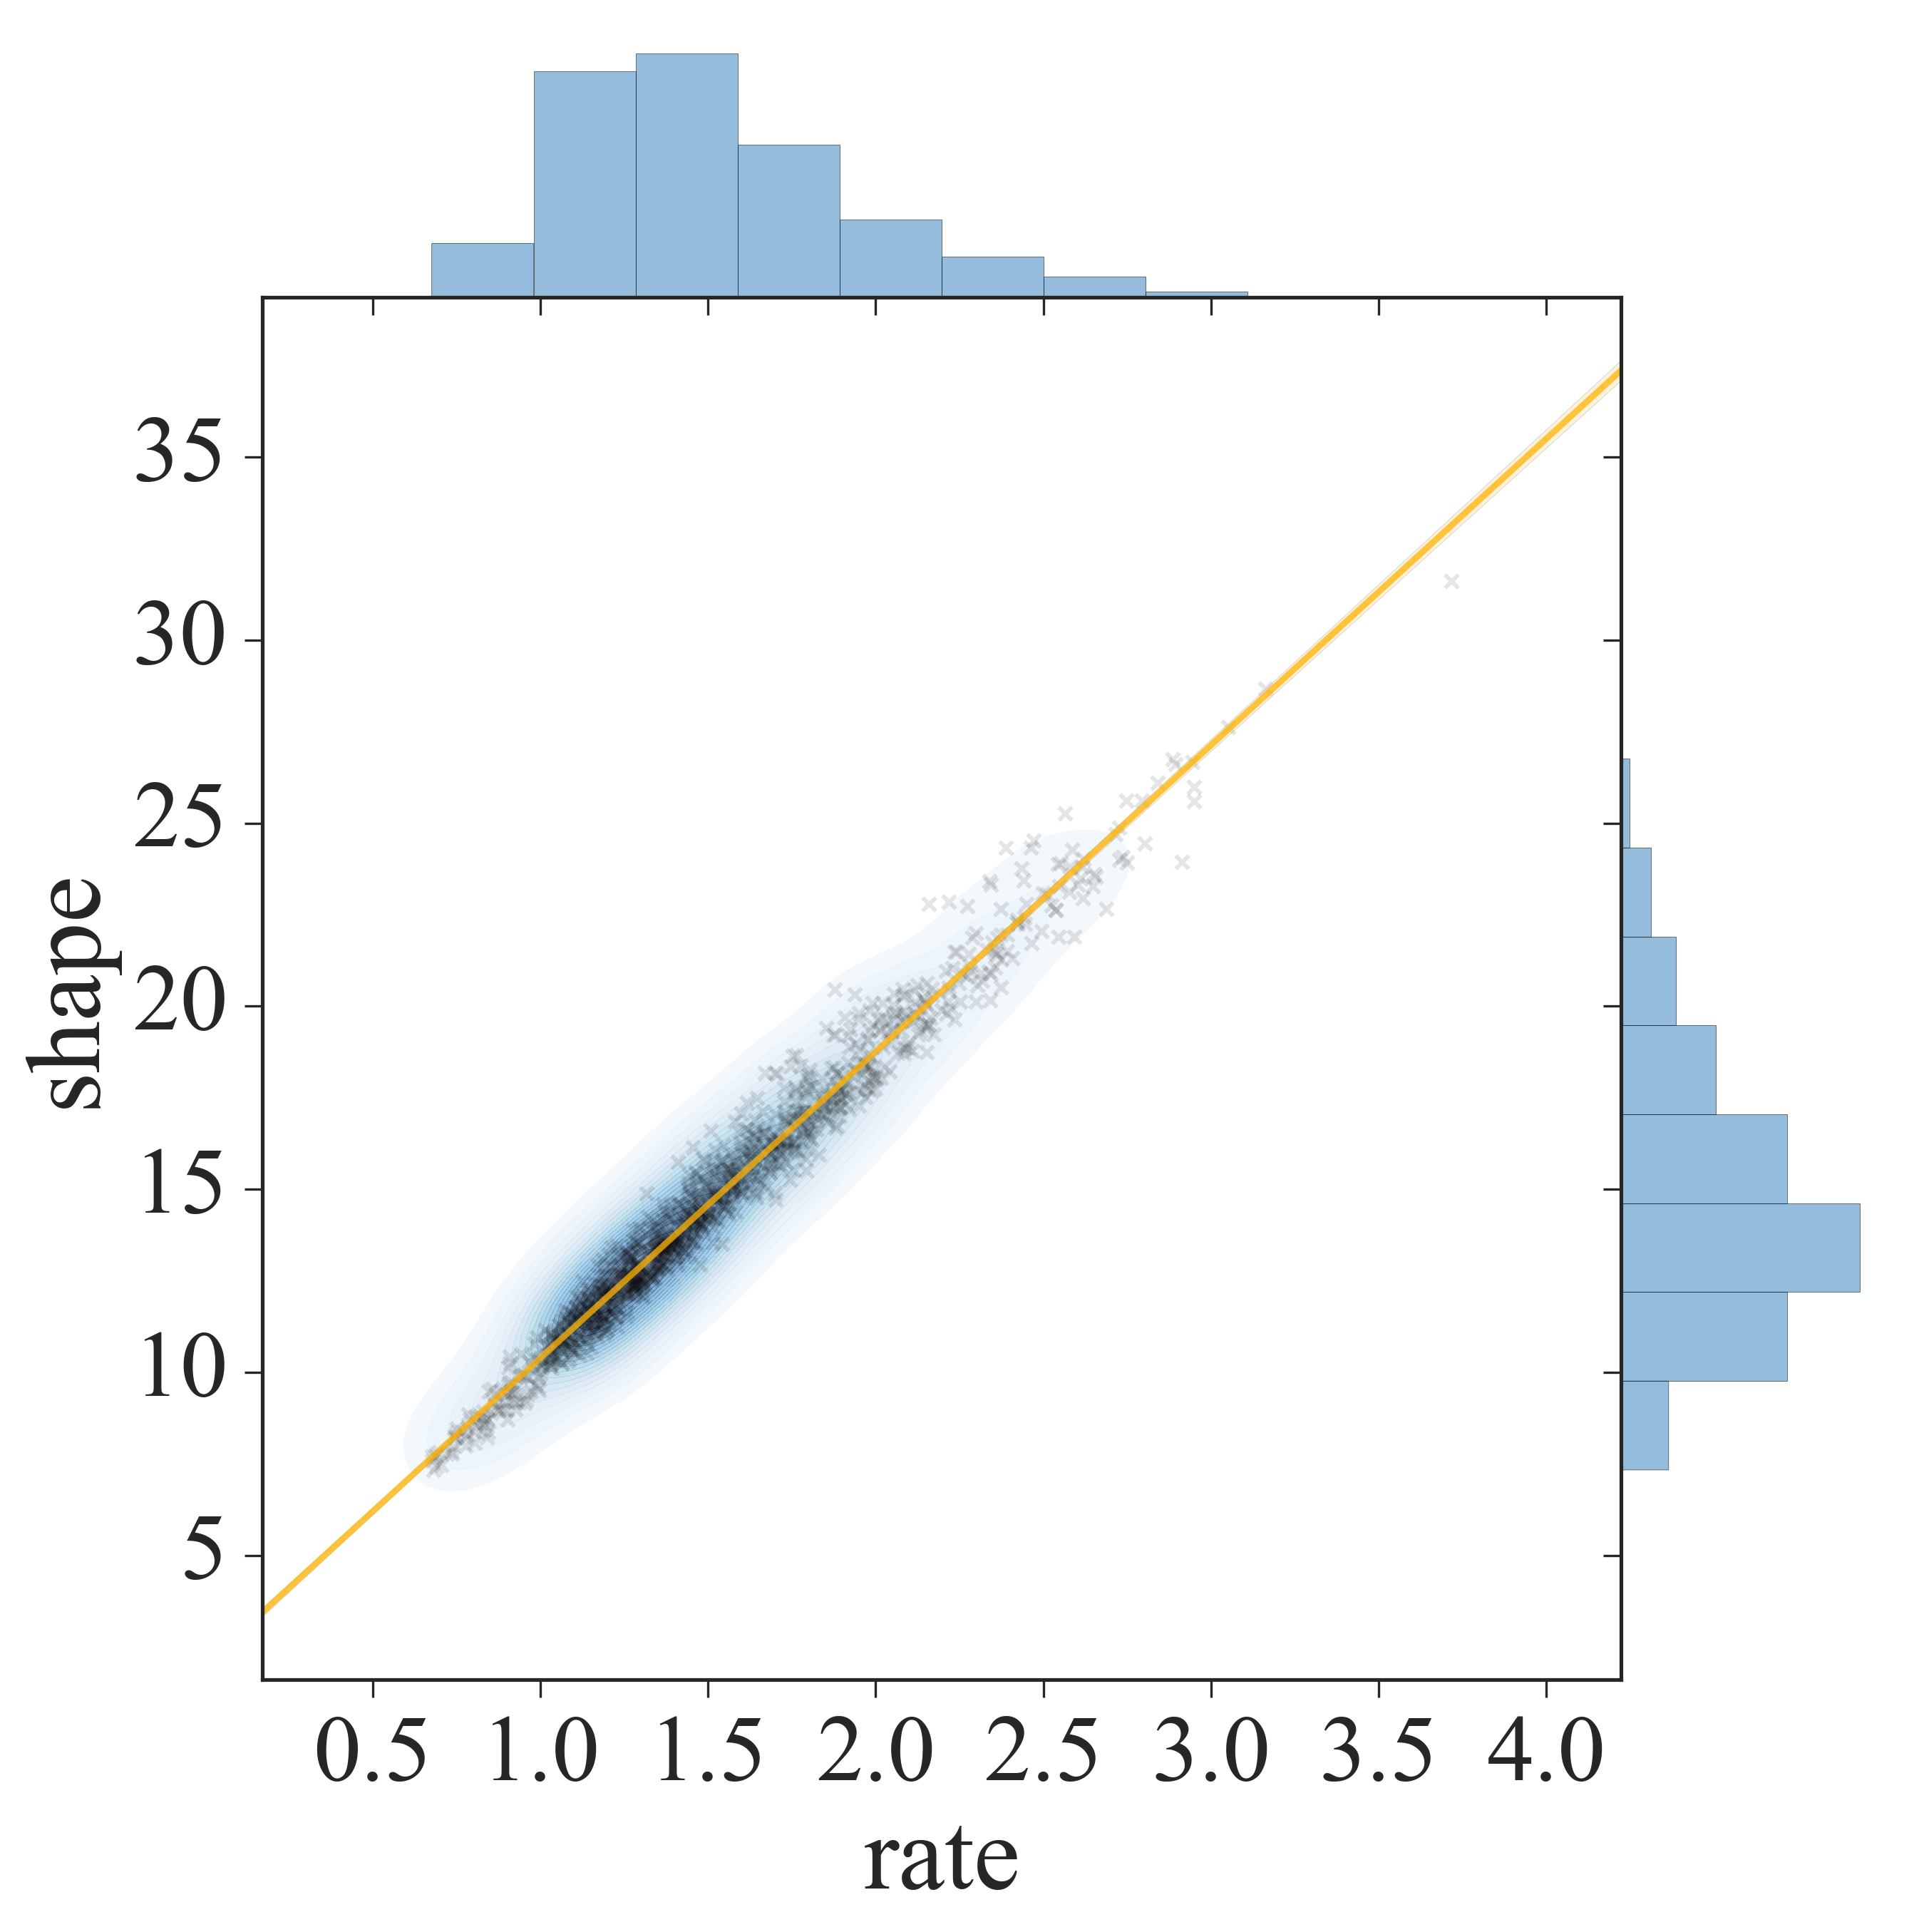
\includegraphics[width=0.75\textwidth]{path_width/physical_edge_width_gamma_fit_rate_shape_scatter_cummulative.png}
			\caption[Path width distribution - Fit parameter densities]{Scatter-plot and kernel density estimates of shape $s$ and rate $r$ for gamma fits of the empirical average path width using the entire dataset. The maximum of the density is located at $s \approx 12.7177$ and $r \approx 1.2799$. A linear fit is shown in yellow.}
			\label{fig:path_widths_gamma_fit_kde}
		\end{figure}

		We remark that earlier work proposed the normal distributions as a suitable description for path widths of coarsened networks that contain a significant number of paths of large width~\cite{baumgarten2010plasmodial}. This is in contrast to the results above, which indicate that within the range of observed parameters, normal distributions are associated with networks where large average path widths are comparatively rare.

		While paths are the atomic constituents of \P their weights do not tell us anything about their arrangement within the graphs. To gain some insight we move on to study the next larger building blocks, namely cycles formed by paths, in the next section.

	\subsection{Face Properties}

		When cultured under the right conditions on flat surfaces, \P forms (almost perfect) $3$-regular planar graphs that have a natural geometric embedding given by the euclidean coordinates of its nodes in the plane ~\cite{baumgarten2010plasmodial}. Each face of the embedding, with the exception of the outer face, is bounded by a cycle of edges. We call such cycles \emph{face cycles} or \emph{faces} for short, see \Fref{fig:graph_schematic}. In other words, faces can be regarded as basic graph building blocks that correspond to loops formed by the veins of the organism. To characterize the structures formed by \P, we study various statistical properties of its faces. Given a graph, all of its faces can be obtained in polynomial time by computing its dual~\cite{mehlhorn1995leda}. 

		Let us stress at this point that the number of faces in our graphs is significantly smaller than the number of nodes or edges. In fact, using Euler's formula for planar graphs and the fact that \P graphs are $3$-regular it is easy to see that the number of faces $f$ is given by $f = 2 + \frac{n}{2}$. As a consequence any statistical observable we compute over the set of faces suffers from smaller sample sizes as compared to path properties for example. Throughout all of our measurements, we ignore outer faces.

		Let us define the degree of a face cycle as the number of degree $3$ nodes it contains.	The cumulative face degree distribution for \series{35} is given in \Fref{fig:face_degree_fit_histogram}. It clearly shows that faces of degree $4$, $5$ and $6$ account for the majority of faces. These findings are consistent across all available data sets. With regards to determining the theoretical distributions, gamma and log-normal fits yield comparable goodness-of-fit plots, with gamma fits being slightly favorable, see \Fref{fig:sup::face_degree_goodness}. Another indication to go with gamma fits is given by similar studies that focus on faces of 2-dimensional Voronoi graphs~\cite{hinde1980monte,tanemura2003statistical}. Since Voronoi graphs are planar, $3$-regular and strongly resembling \P graphs, gamma fits can be expected to be a good choice. It is interesting to note that for Voronoi graphs faces of degree $6$ are known to have the largest expectation. We remark at this point, that the time development of the fit parameters shown in \Fref{fig:face_degree_fit_parameters} shows rather large values of shape, which indicates that the gamma distribution is approaching a normal distribution. Furthermore, a linear relationship between shape $s$ and rate $r$ is apparent.
 
		\begin{figure}
			\centering
			\subfloat[][]{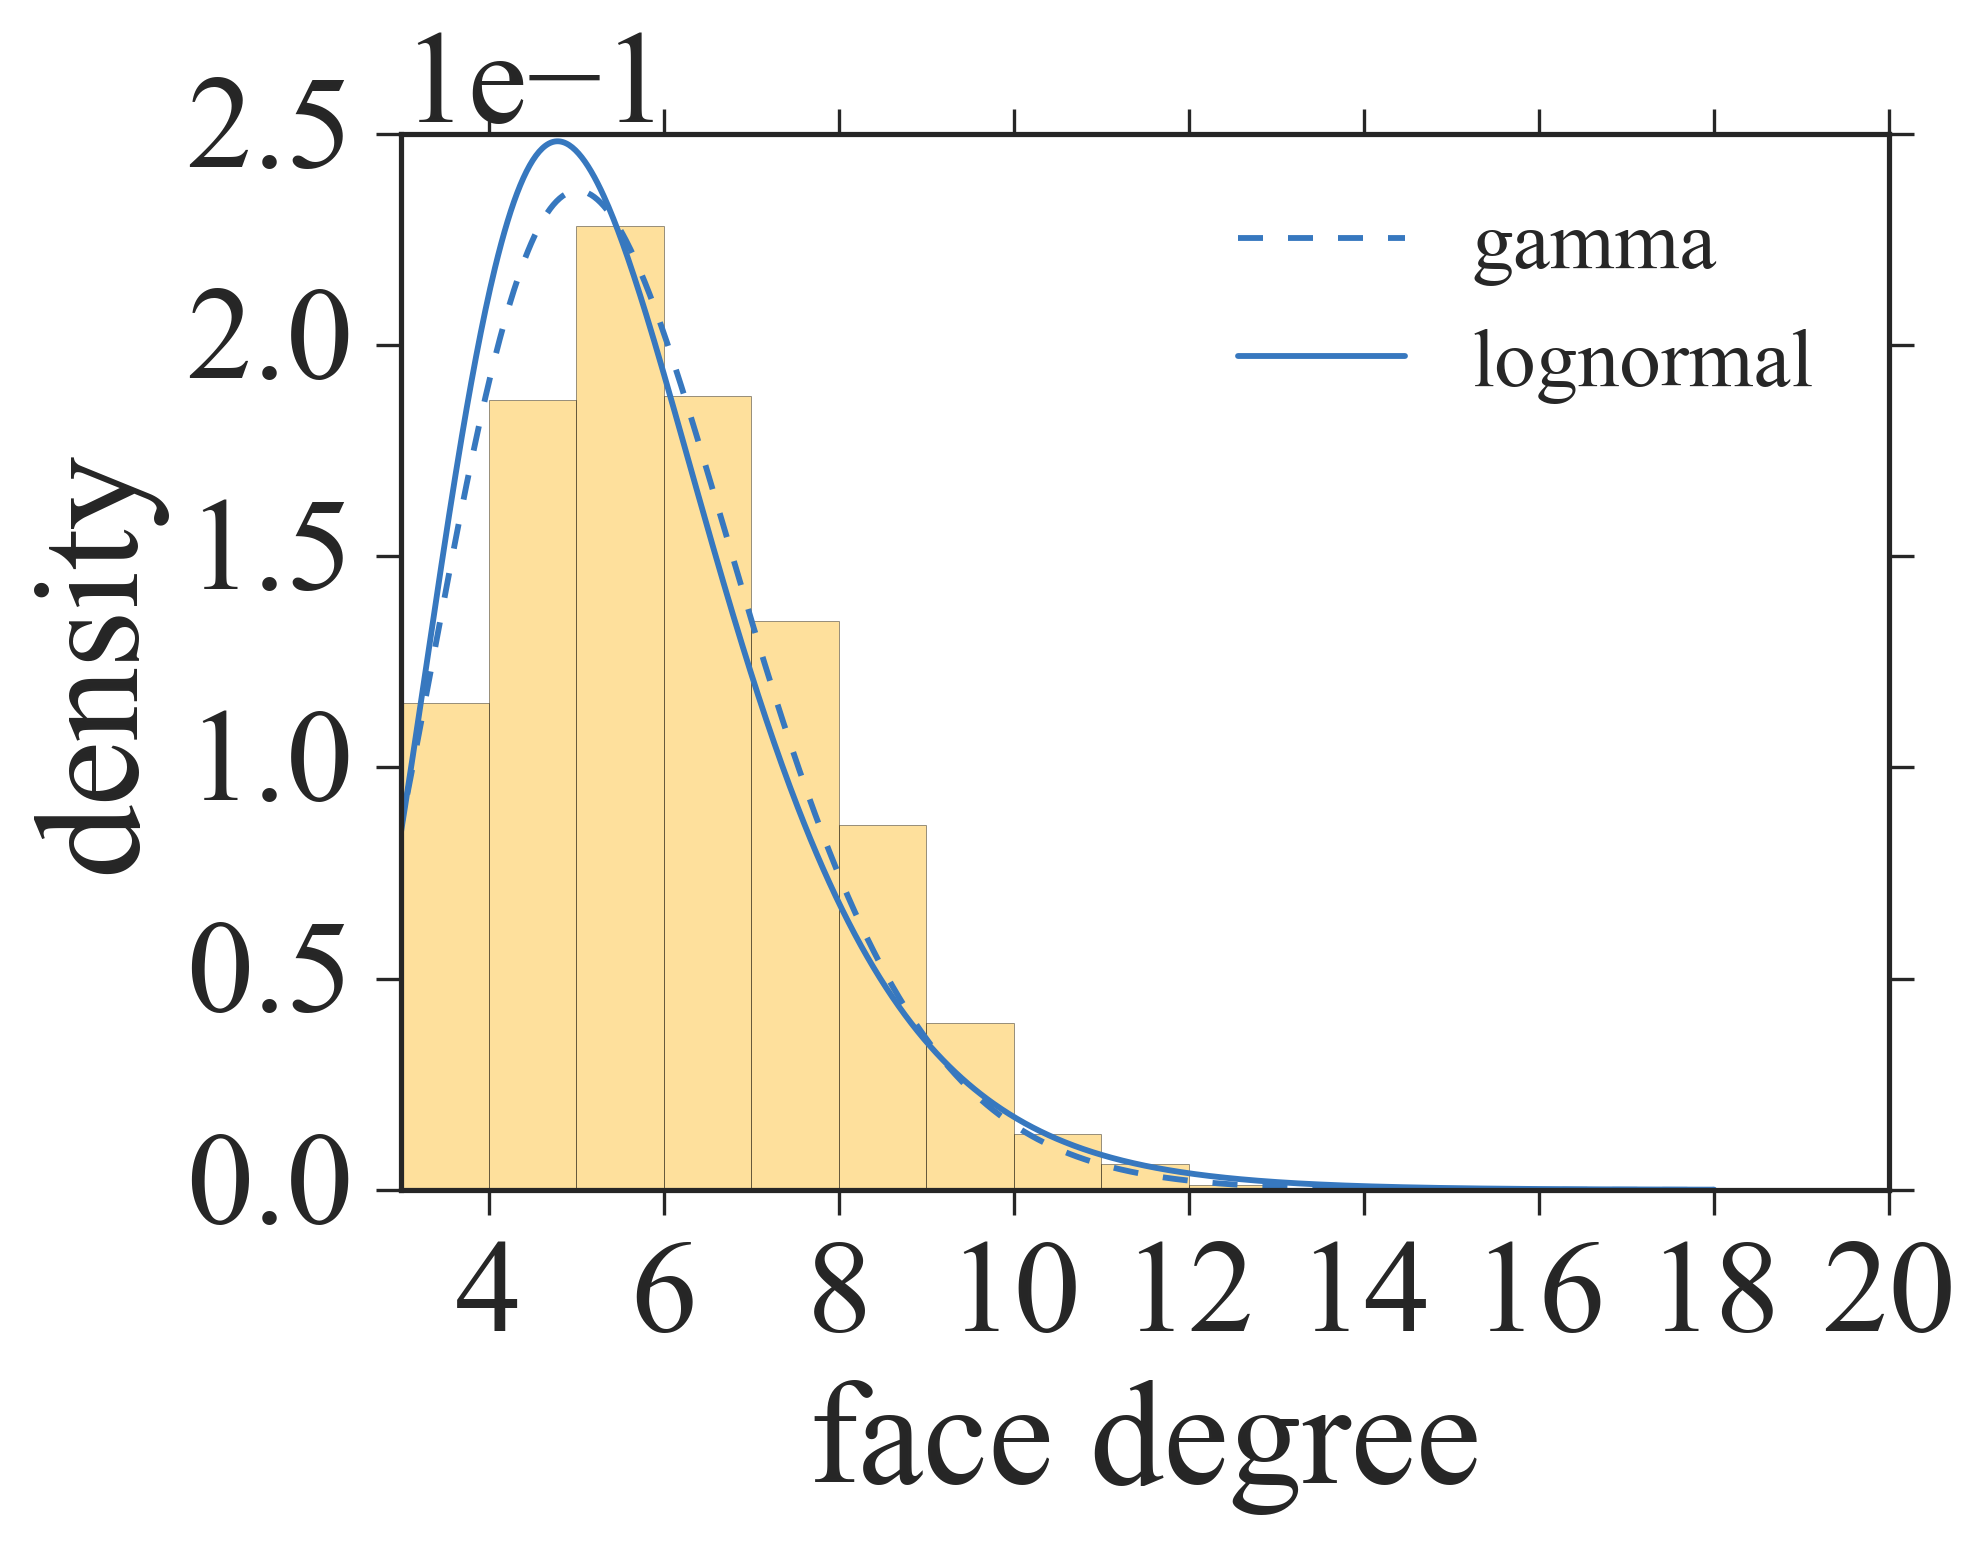
\includegraphics[width=\twoimageswide,keepaspectratio]{face_degree/face_degree_motion35.png}
			\label{fig:face_degree_fit_histogram}}\qquad
			\subfloat[][]{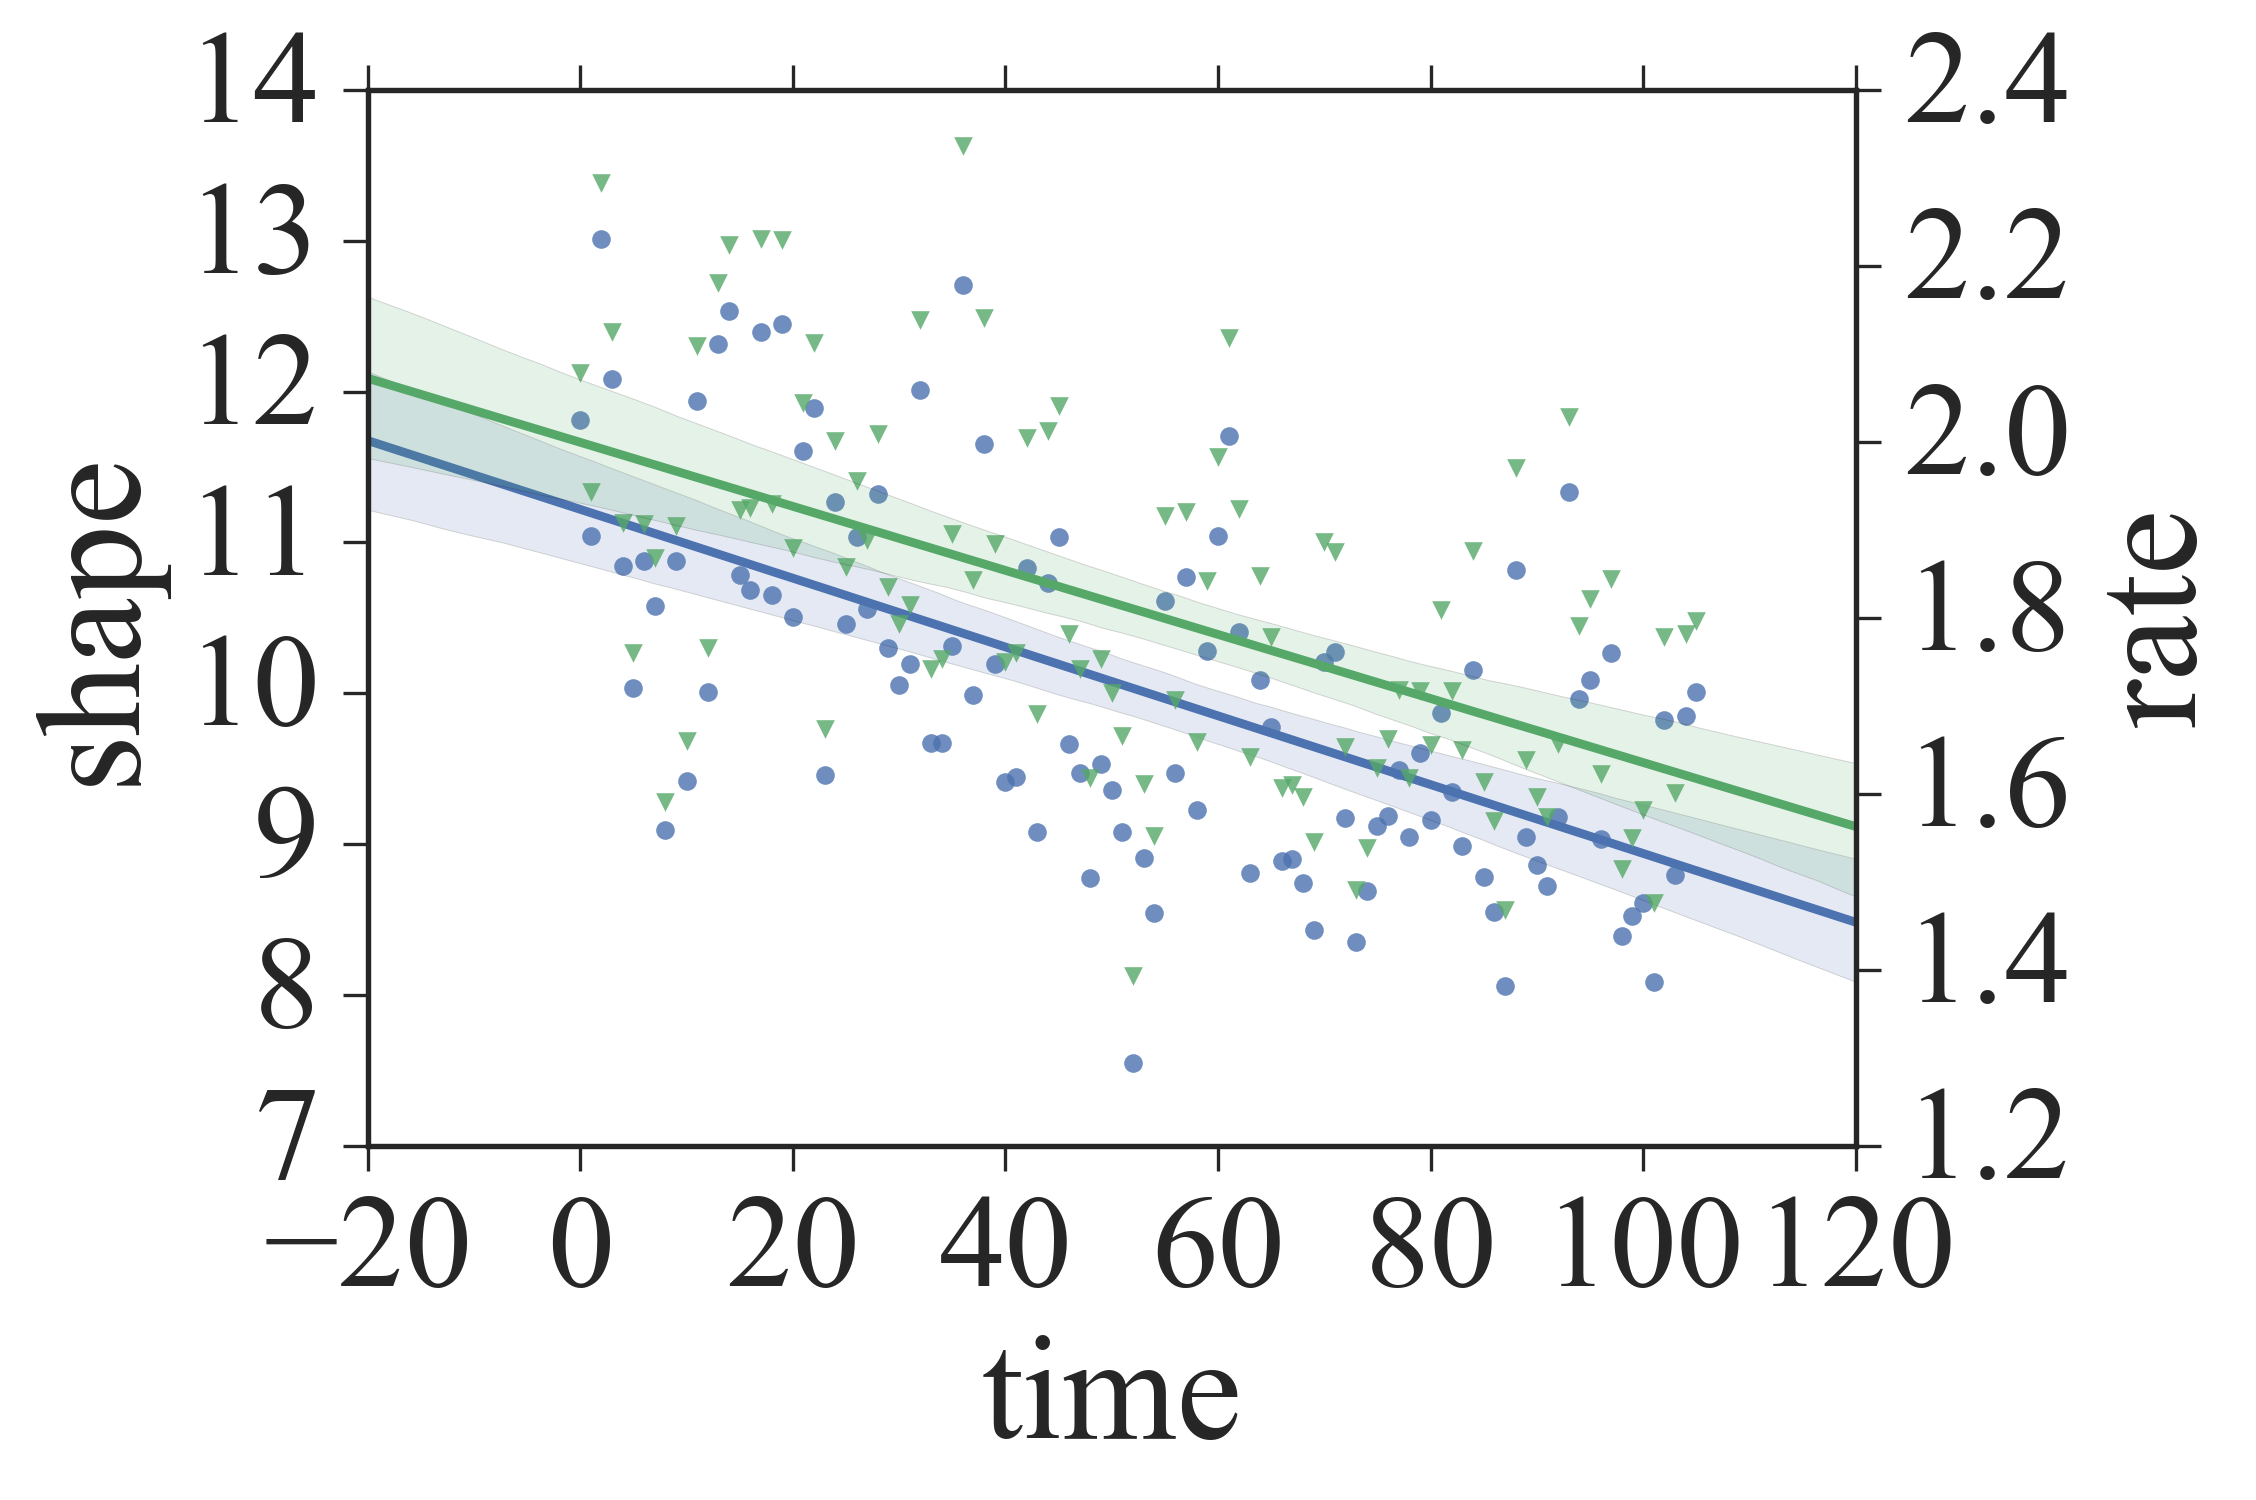
\includegraphics[width=\twoimageswide,keepaspectratio]{face_degree/dual_node_degree_gamma_fit_parameters_together_motion35.png}
			\label{fig:face_degree_fit_parameters}}

			\caption[Face degree distribution]{(a): Cumulative empirical face degree distribution for \series{35}. Candidate gamma and log normal fits are shown. (b): Gamma fit parameters shape (blue circles) and rate (green triangles) as a function of time for the same series. Linear fits are shown to guide the eye. Abscissa in units of \SI{120}{\second}.}
			\label{fig:face_degree_fit}
		\end{figure}

		\Fref{fig:face_degree_kde} shows that this relation is valid across the entire dataset and is given by $s(r) = (\num{5.3403 \pm 0.021}) r + (\num{0.3508 \pm 0.037})$.
 
		\begin{figure}[!htbp]
			\centering
				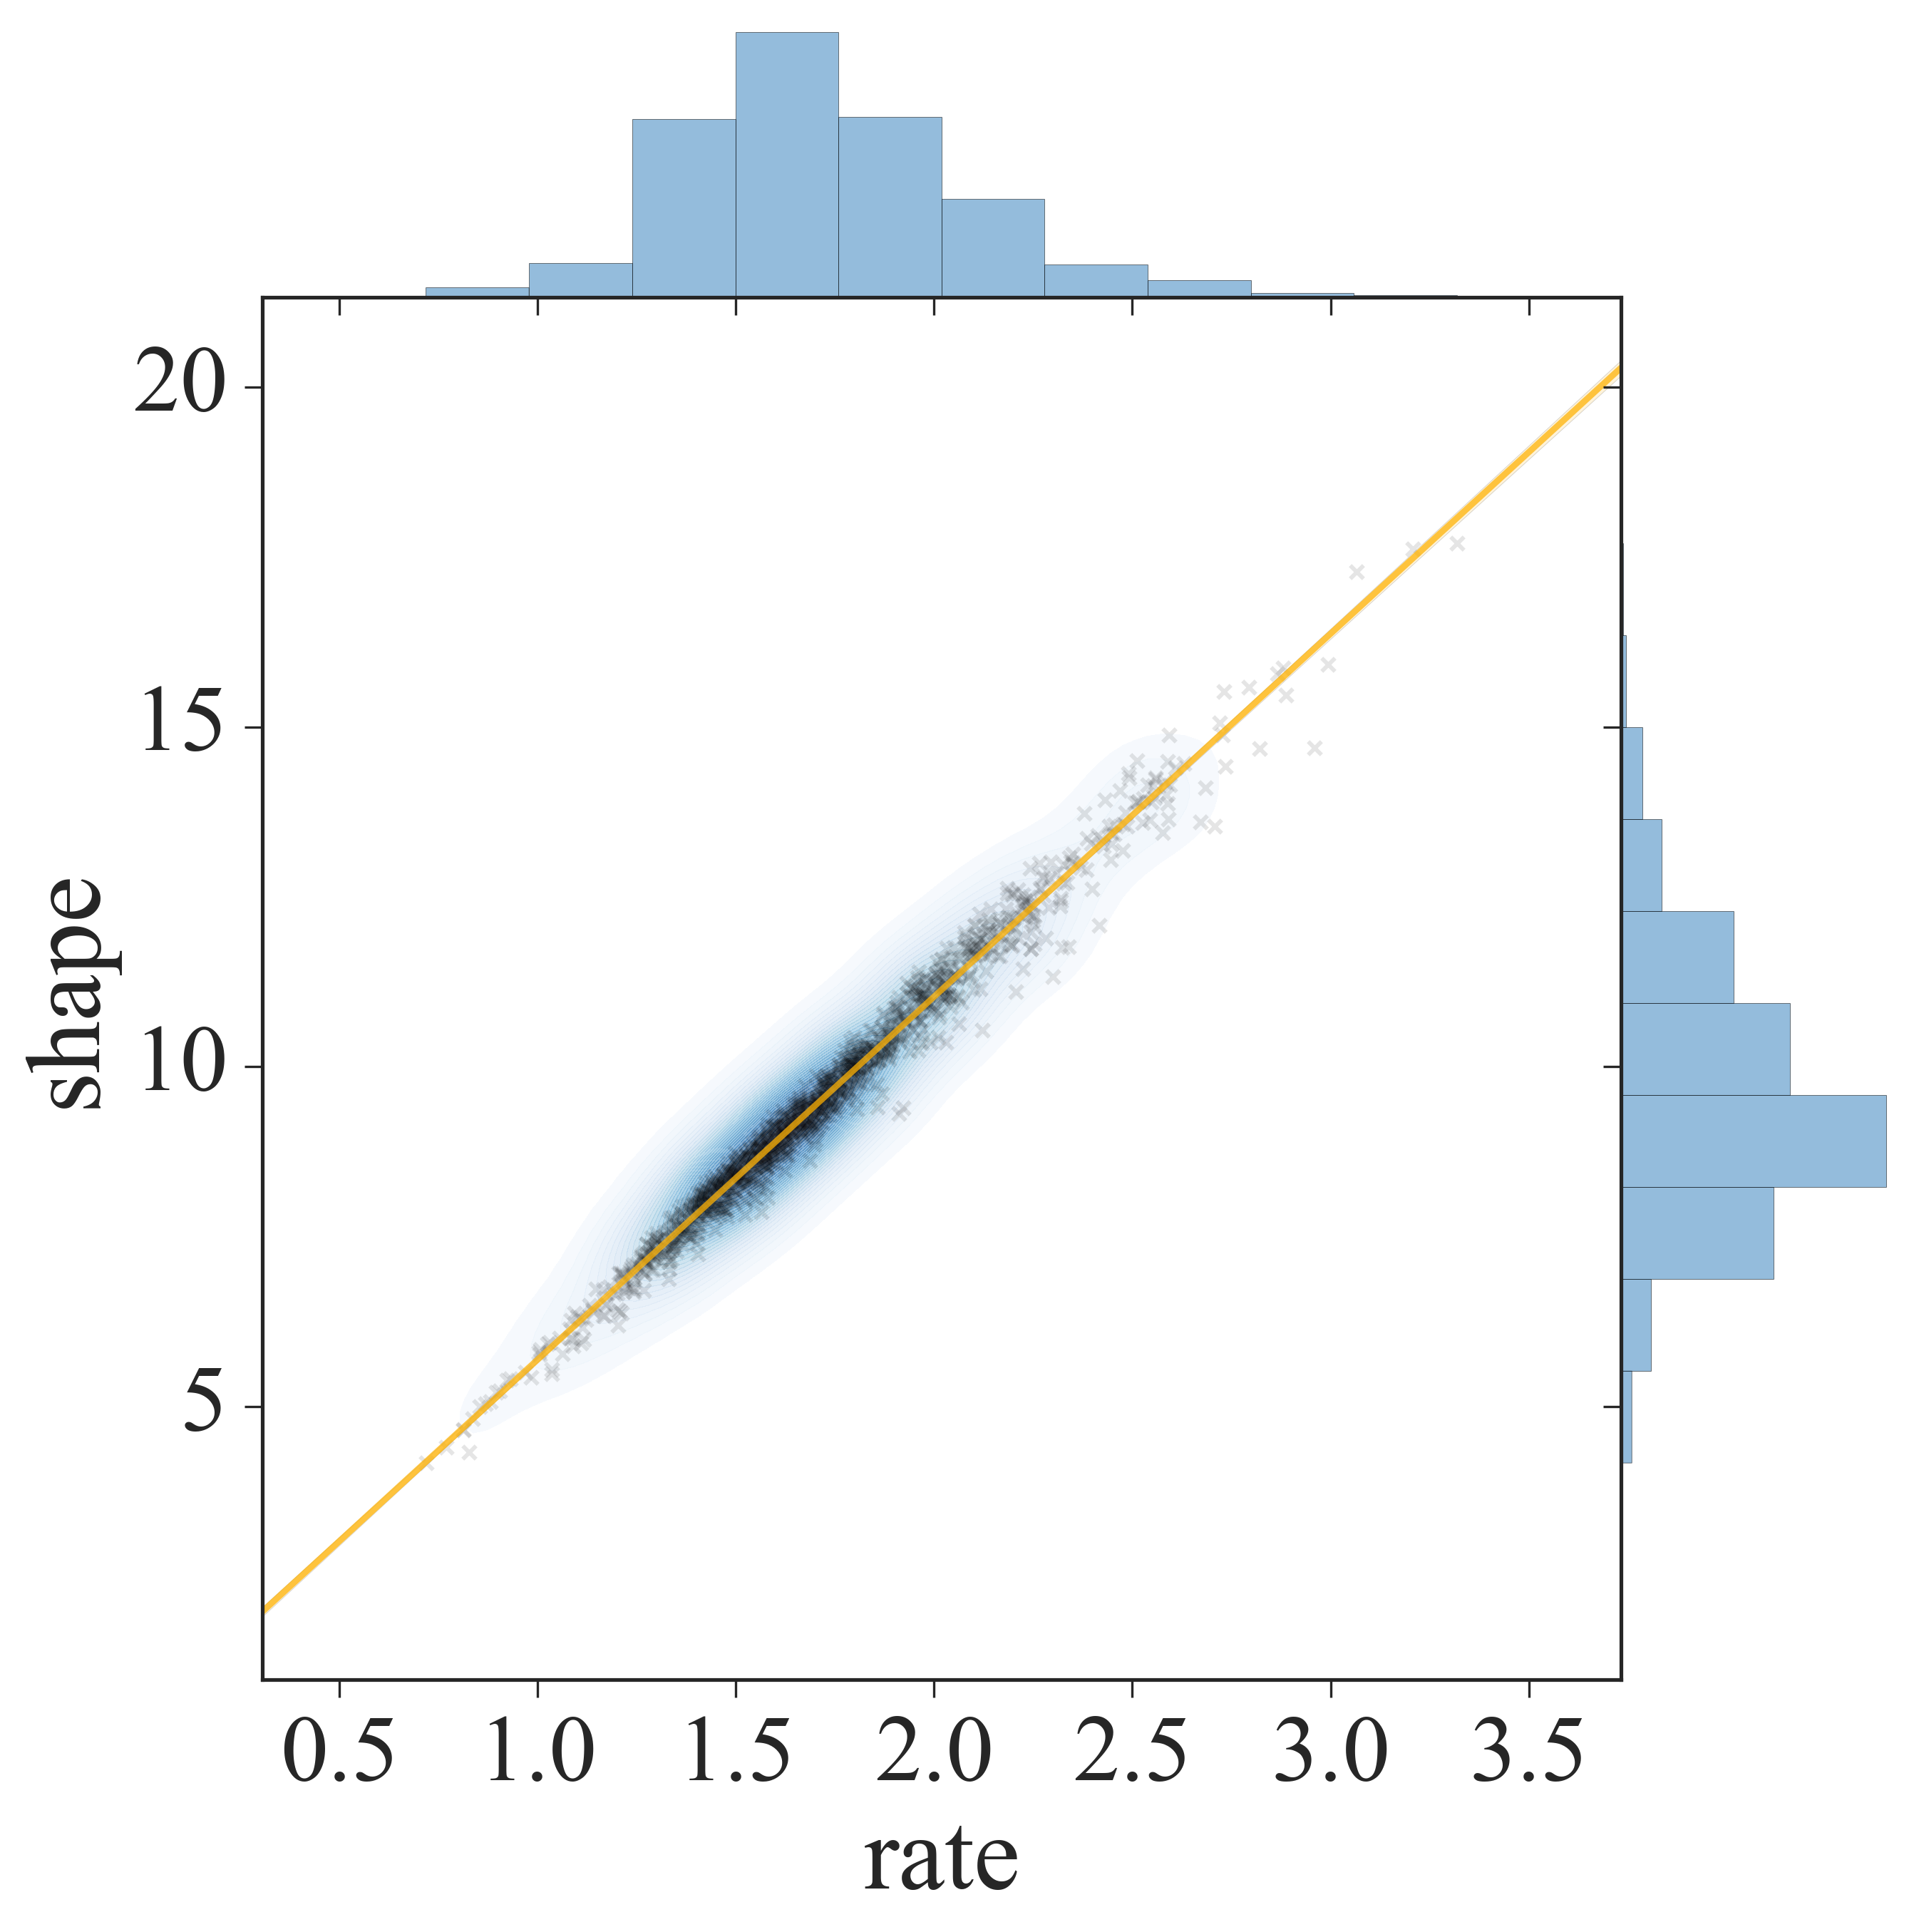
\includegraphics[width=0.75\textwidth]{face_degree/dual_node_degree_gamma_fit_rate_shape_scatter_cummulative.png}
			\caption[Face degree distribution - Fit parameter densities]{Scatter-plot and kernel density estimates of shape $s$ and rate $r$ for gamma fits of the empirical face degrees using the entire dataset. The maximum of the density is located at $s \approx 9.0387$ and $r \approx 1.6255$.}
			\label{fig:face_degree_kde}
		\end{figure}

		Given this relation we may parametrize the gamma distribution as a function of $r$ and study the behavior of the mode as $r$ takes on values in $[1,3]$. Again we find that the possible positions of the mode are restricted to a rather small interval given by $[4.6911,5.1239]$. For $r = 1.6255$, which is associated with the maximum in the density plot of \Fref{fig:face_degree_kde}, the mode takes a value of $4.941$. Rounding these values to the nearest integer suggests that a mode of $5$ is most likely to be found for a randomly picked face of a \P graphs.

		Analogous to the discussion of the path widths, for a data series to exhibit a high density of large degree faces, small values of $r$ are necessary. \Fref{fig:face_degree_fit_parameters} indicates that the underlying networks of \series{35} are actively changing as to increase the number of large degree faces while keeping the distribution mode largely constant. While we find this behavior for many data series, there are others which seem to keep the degree distribution largely stable. The reasons for this are unclear at this point.


		Next we investigate the empirical distributions of the areas enclosed by faces in more detail. The cumulative face area distribution for \series{35} is given in \Fref{fig:face_area_fit_histogram}. It's goodness-of-fit plots suggest that a gamma fit yields a reliable description of the empirical data, see \Fref{fig:sup::face_area_goodness}. The time development of the associated fit parameters is given in \Fref{fig:face_area_fit_parameters}. Note that the shape values fall below $1$ repeatedly, which prevents us from using the mode to characterize the most likely face areas since it requires $s >1$. However, analogous to earlier results, increasing values of $s$ in combination with decreasing values of $r$ indicate that the probability mass of the associated gamma distribution is shifting towards larger face areas. Given the time development depicted in \Fref{fig:face_area_fit_parameters}, this is consistent with network coarsening.

		We stress that, while a gamma distribution yields a good description of \series{35}, for numerous other data series gamma fits perform poorly in the center of the distributions compared to a log-normal distribution. The fact that the face area data exhibits a large degree of variance in combination with the reduced size of the available data points hampers our ability to properly select a fitting theoretical description. Results associated with log-normal fits are available in the full data collection.

		\begin{figure}
			\centering
			\subfloat[][]{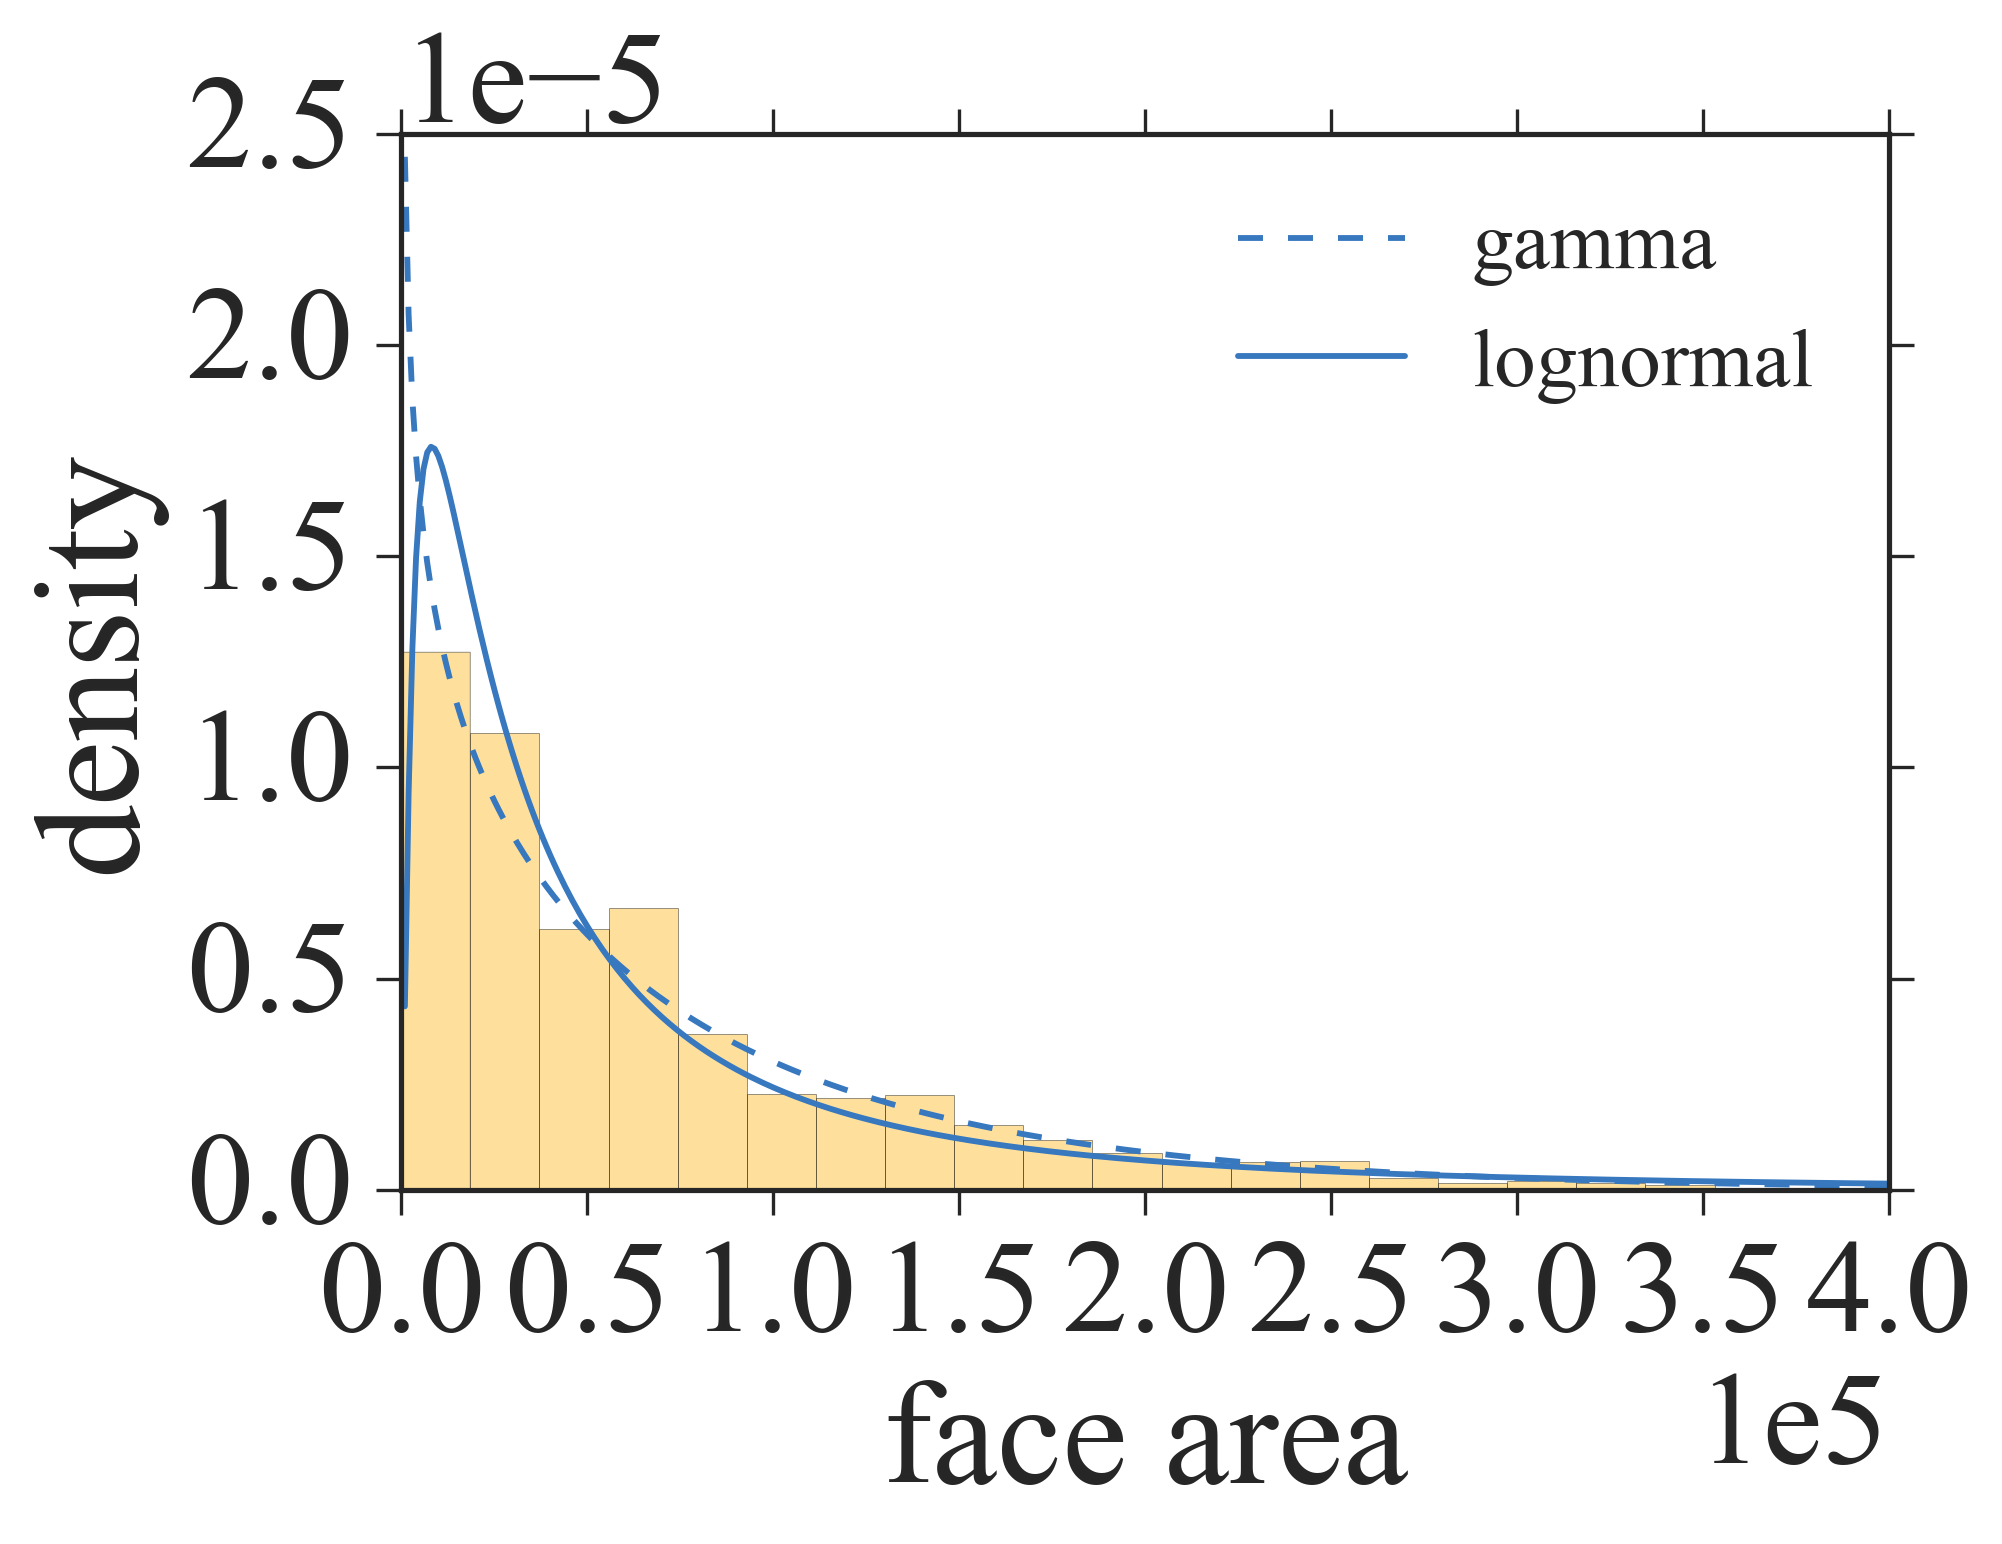
\includegraphics[width=\twoimageswide,keepaspectratio]{face_area/face_area_motion35.png}
			\label{fig:face_area_fit_histogram}}\qquad
			\subfloat[][]{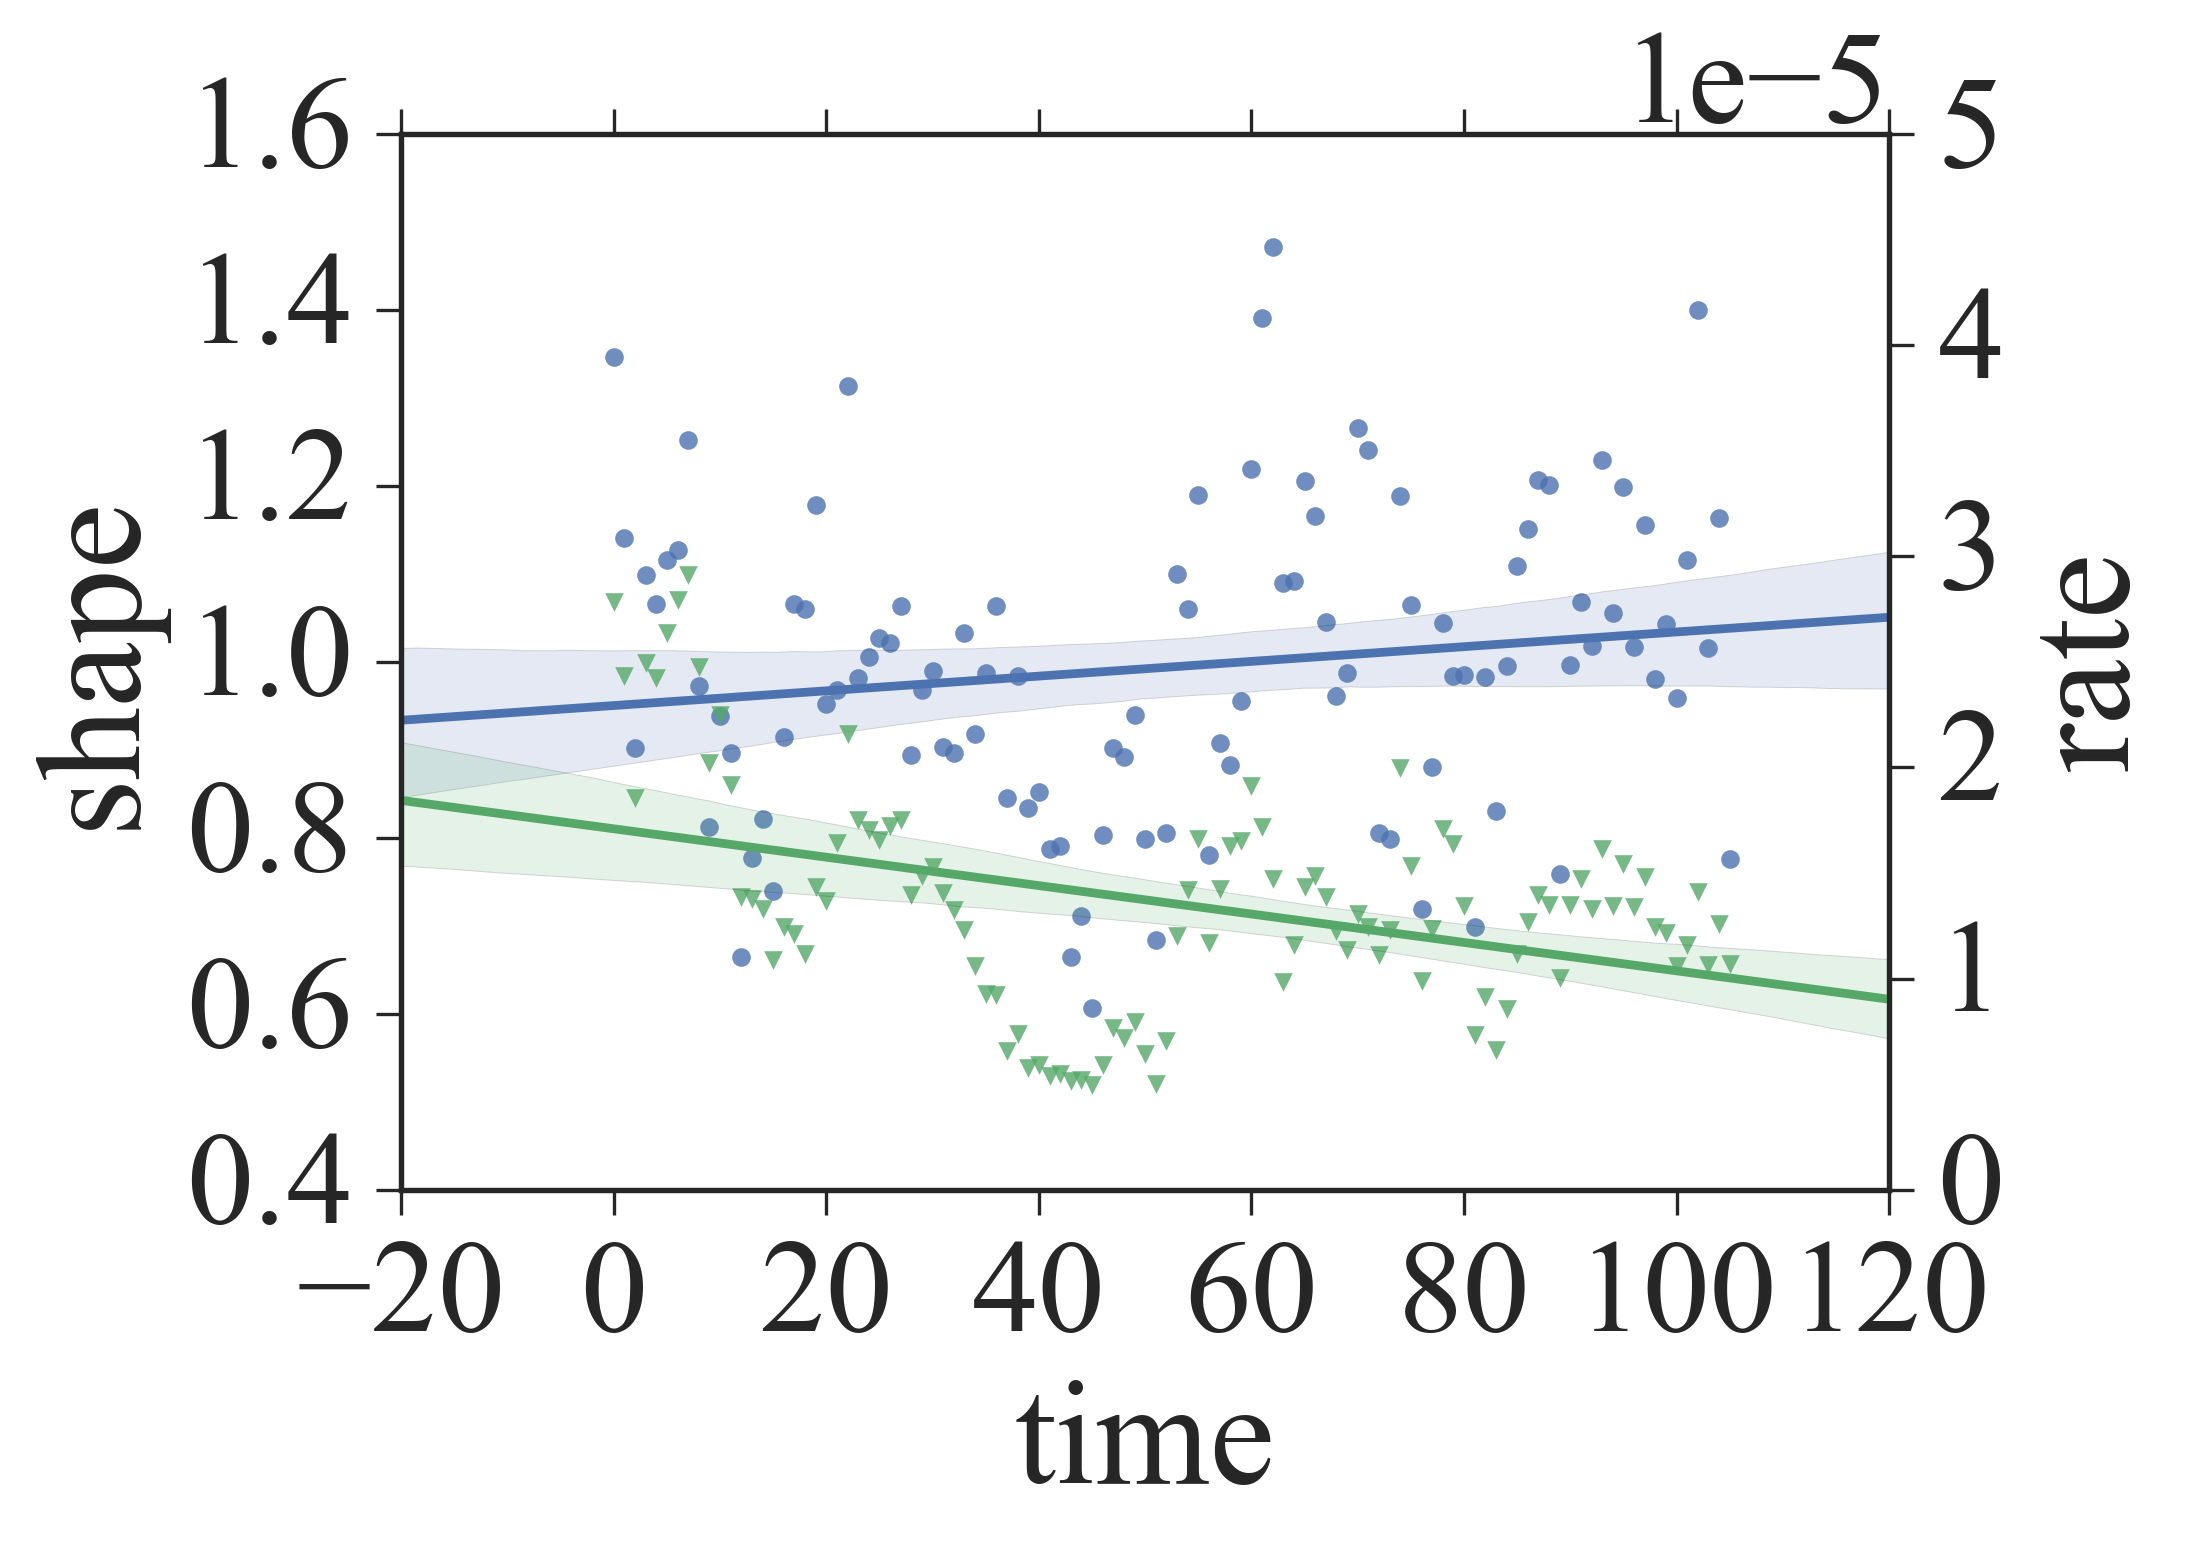
\includegraphics[width=\twoimageswide,keepaspectratio]{face_area/face_area_gamma_fit_parameters_together_motion35.png}
			\label{fig:face_area_fit_parameters}}

			\caption[Face area distribution]{(a): Cumulative empirical face area distribution for \series{35}. Candidate gamma and log normal fits are shown. Abscissa in units of \si{\pixel\squared}. (b): Gamma fit parameters shape (blue circles) and rate (green triangles) as a function of time for the same series. Linear fits are shown to guide the eye. Abscissa in units of \SI{120}{\second}.}
			\label{fig:face_area_fit}
		\end{figure}


		A global impression of what ranges of fit parameter one can expect to encounter for gamma fits of the empirical face area distributions is given in \Fref{fig:face_area_kde}. 

		\begin{figure}[!htbp]
			\centering
				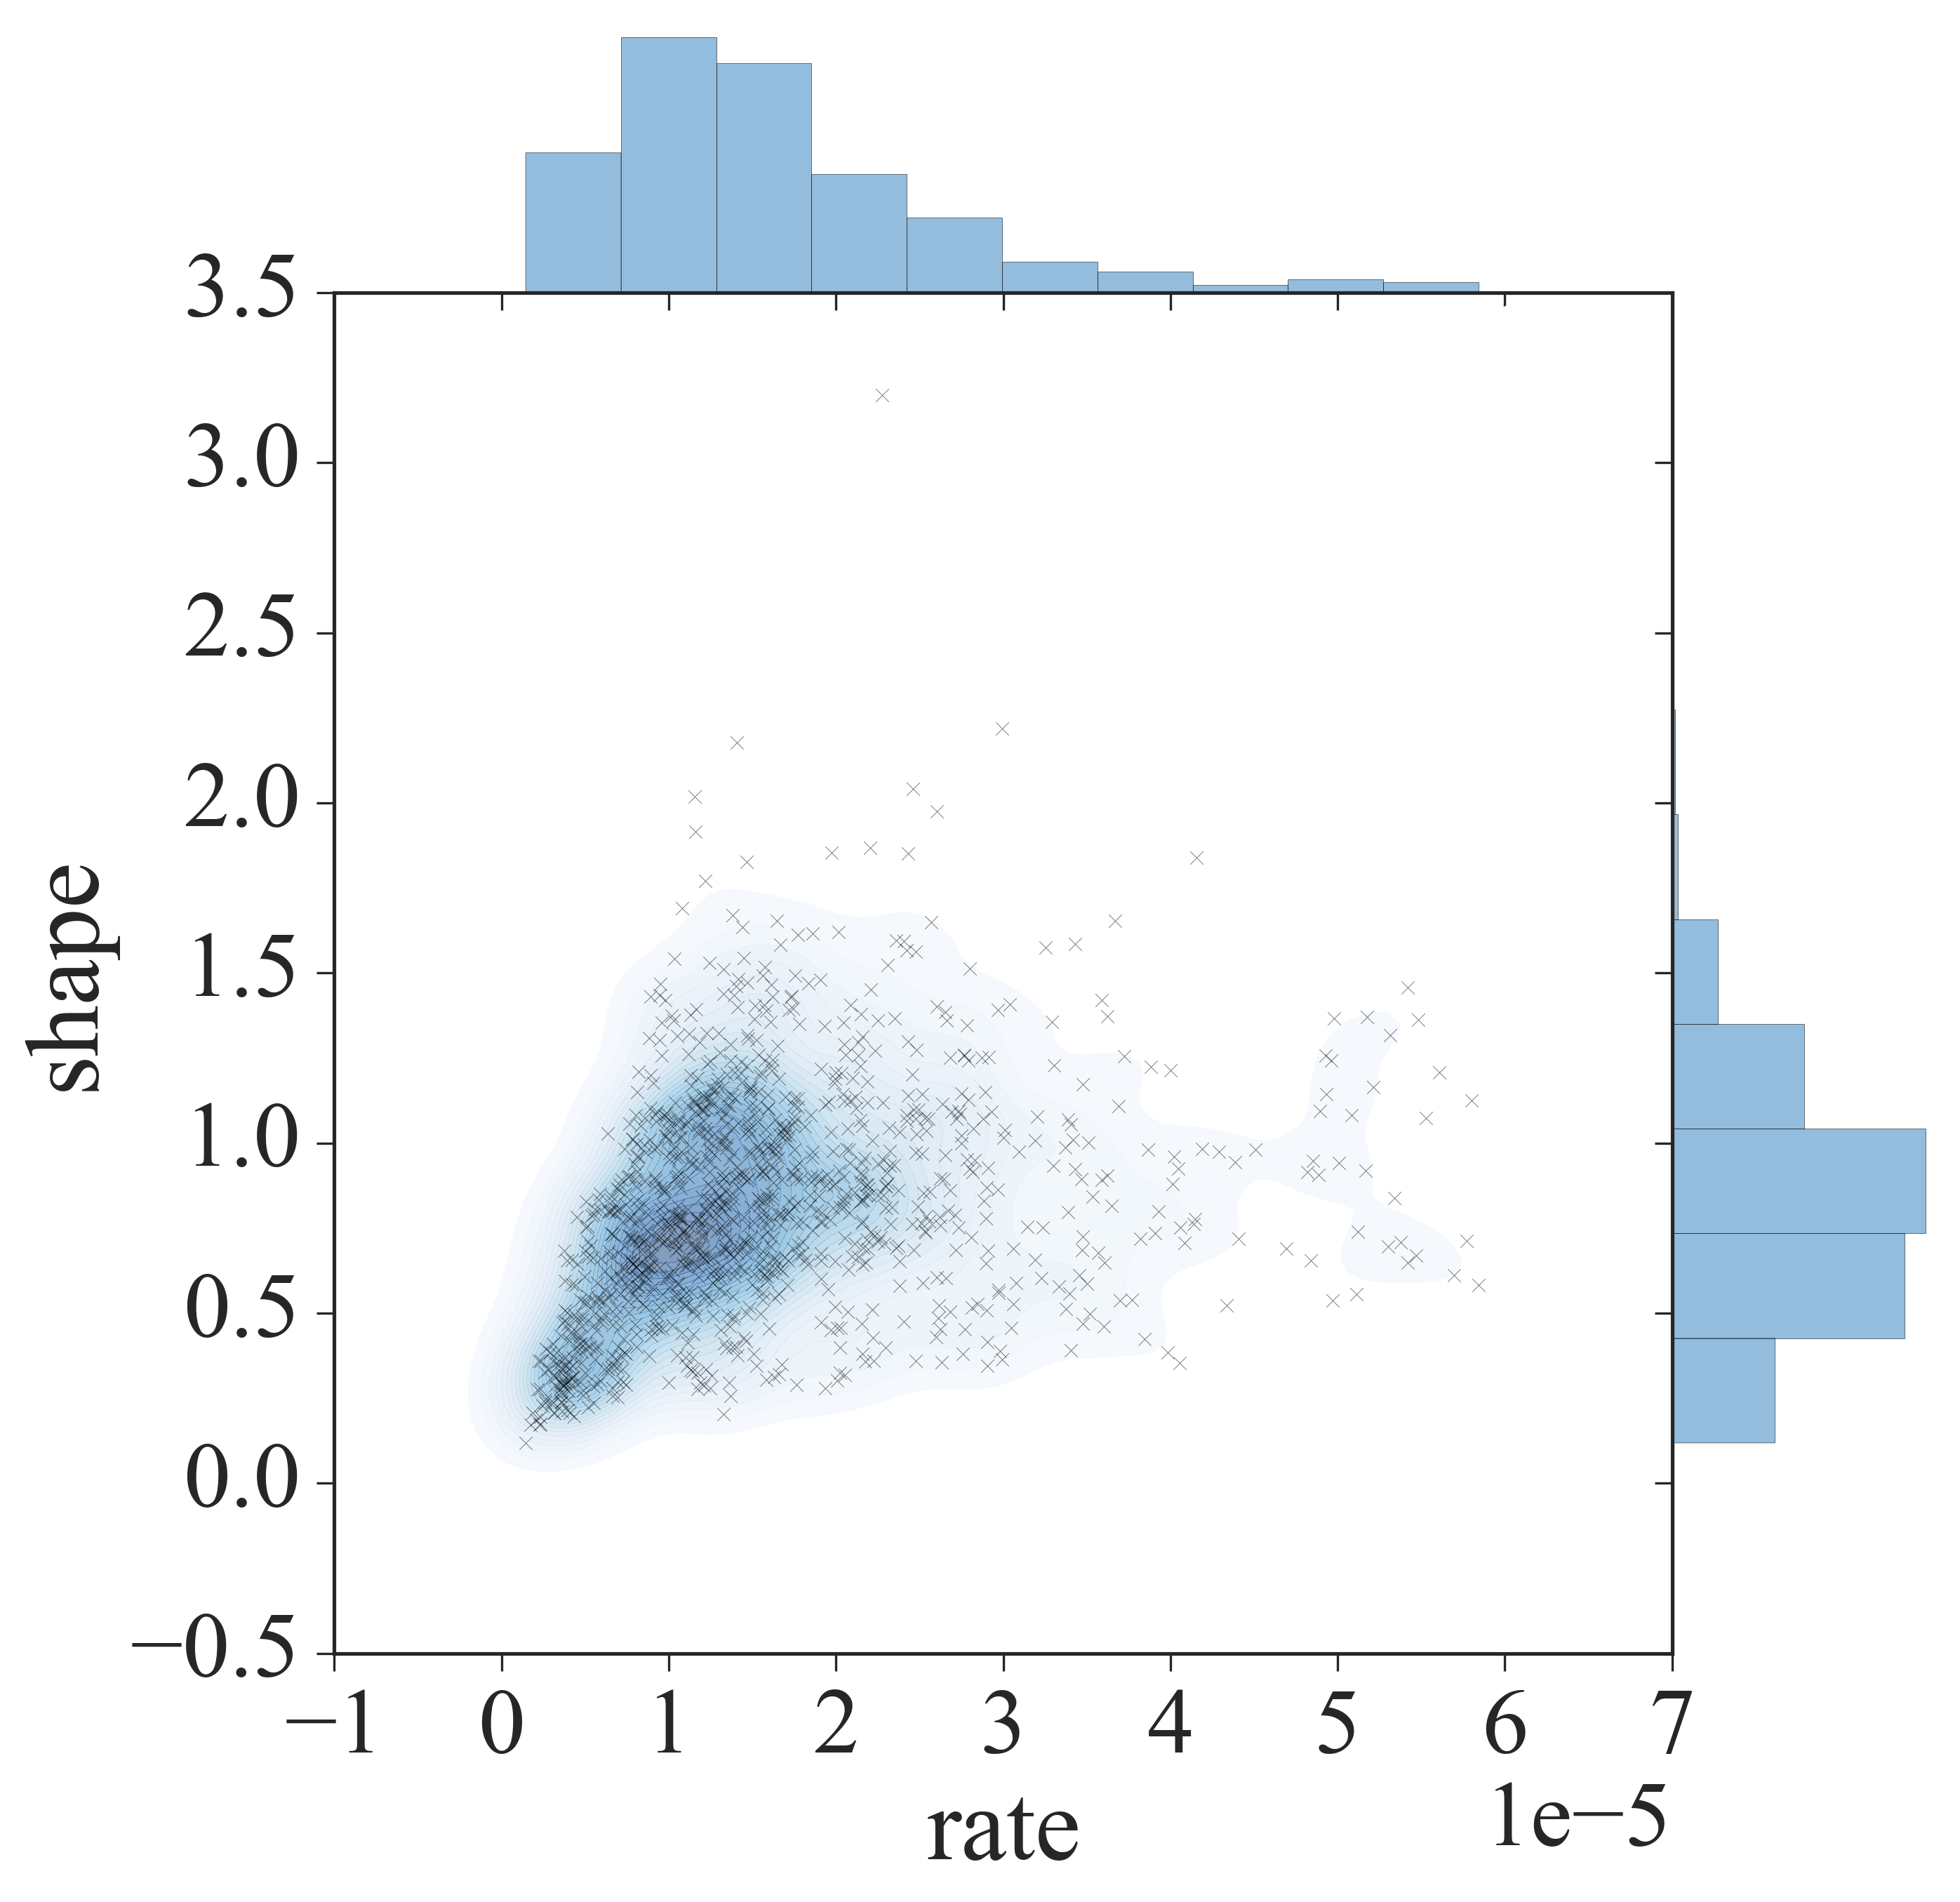
\includegraphics[width=0.75\textwidth]{face_area/face_area_gamma_fit_rate_shape_scatter_cummulative.png}
			\caption[Face area distribution - Fit parameter densities]{Scatter-plot and kernel density estimates of shape $s$ and rate $r$ for gamma fits of the empirical face areas using the entire dataset. The maximum of the density is located at $s \approx 0.7022$ and $r \approx 1.0381 \times 10^{-5}$.}
			\label{fig:face_area_kde}
		\end{figure}

		Finally, \Fref{fig:face_degree_per_area} shows how the sum of the area covered by all faces across all data series is distributed with respect to face degree. It can be seen that faces of degree $6$ and $7$ account for the majority of the area covered, while faces of degree $5$ and $8$ play a smaller role in comparison. 

		\begin{figure}[!htbp]
			\centering
				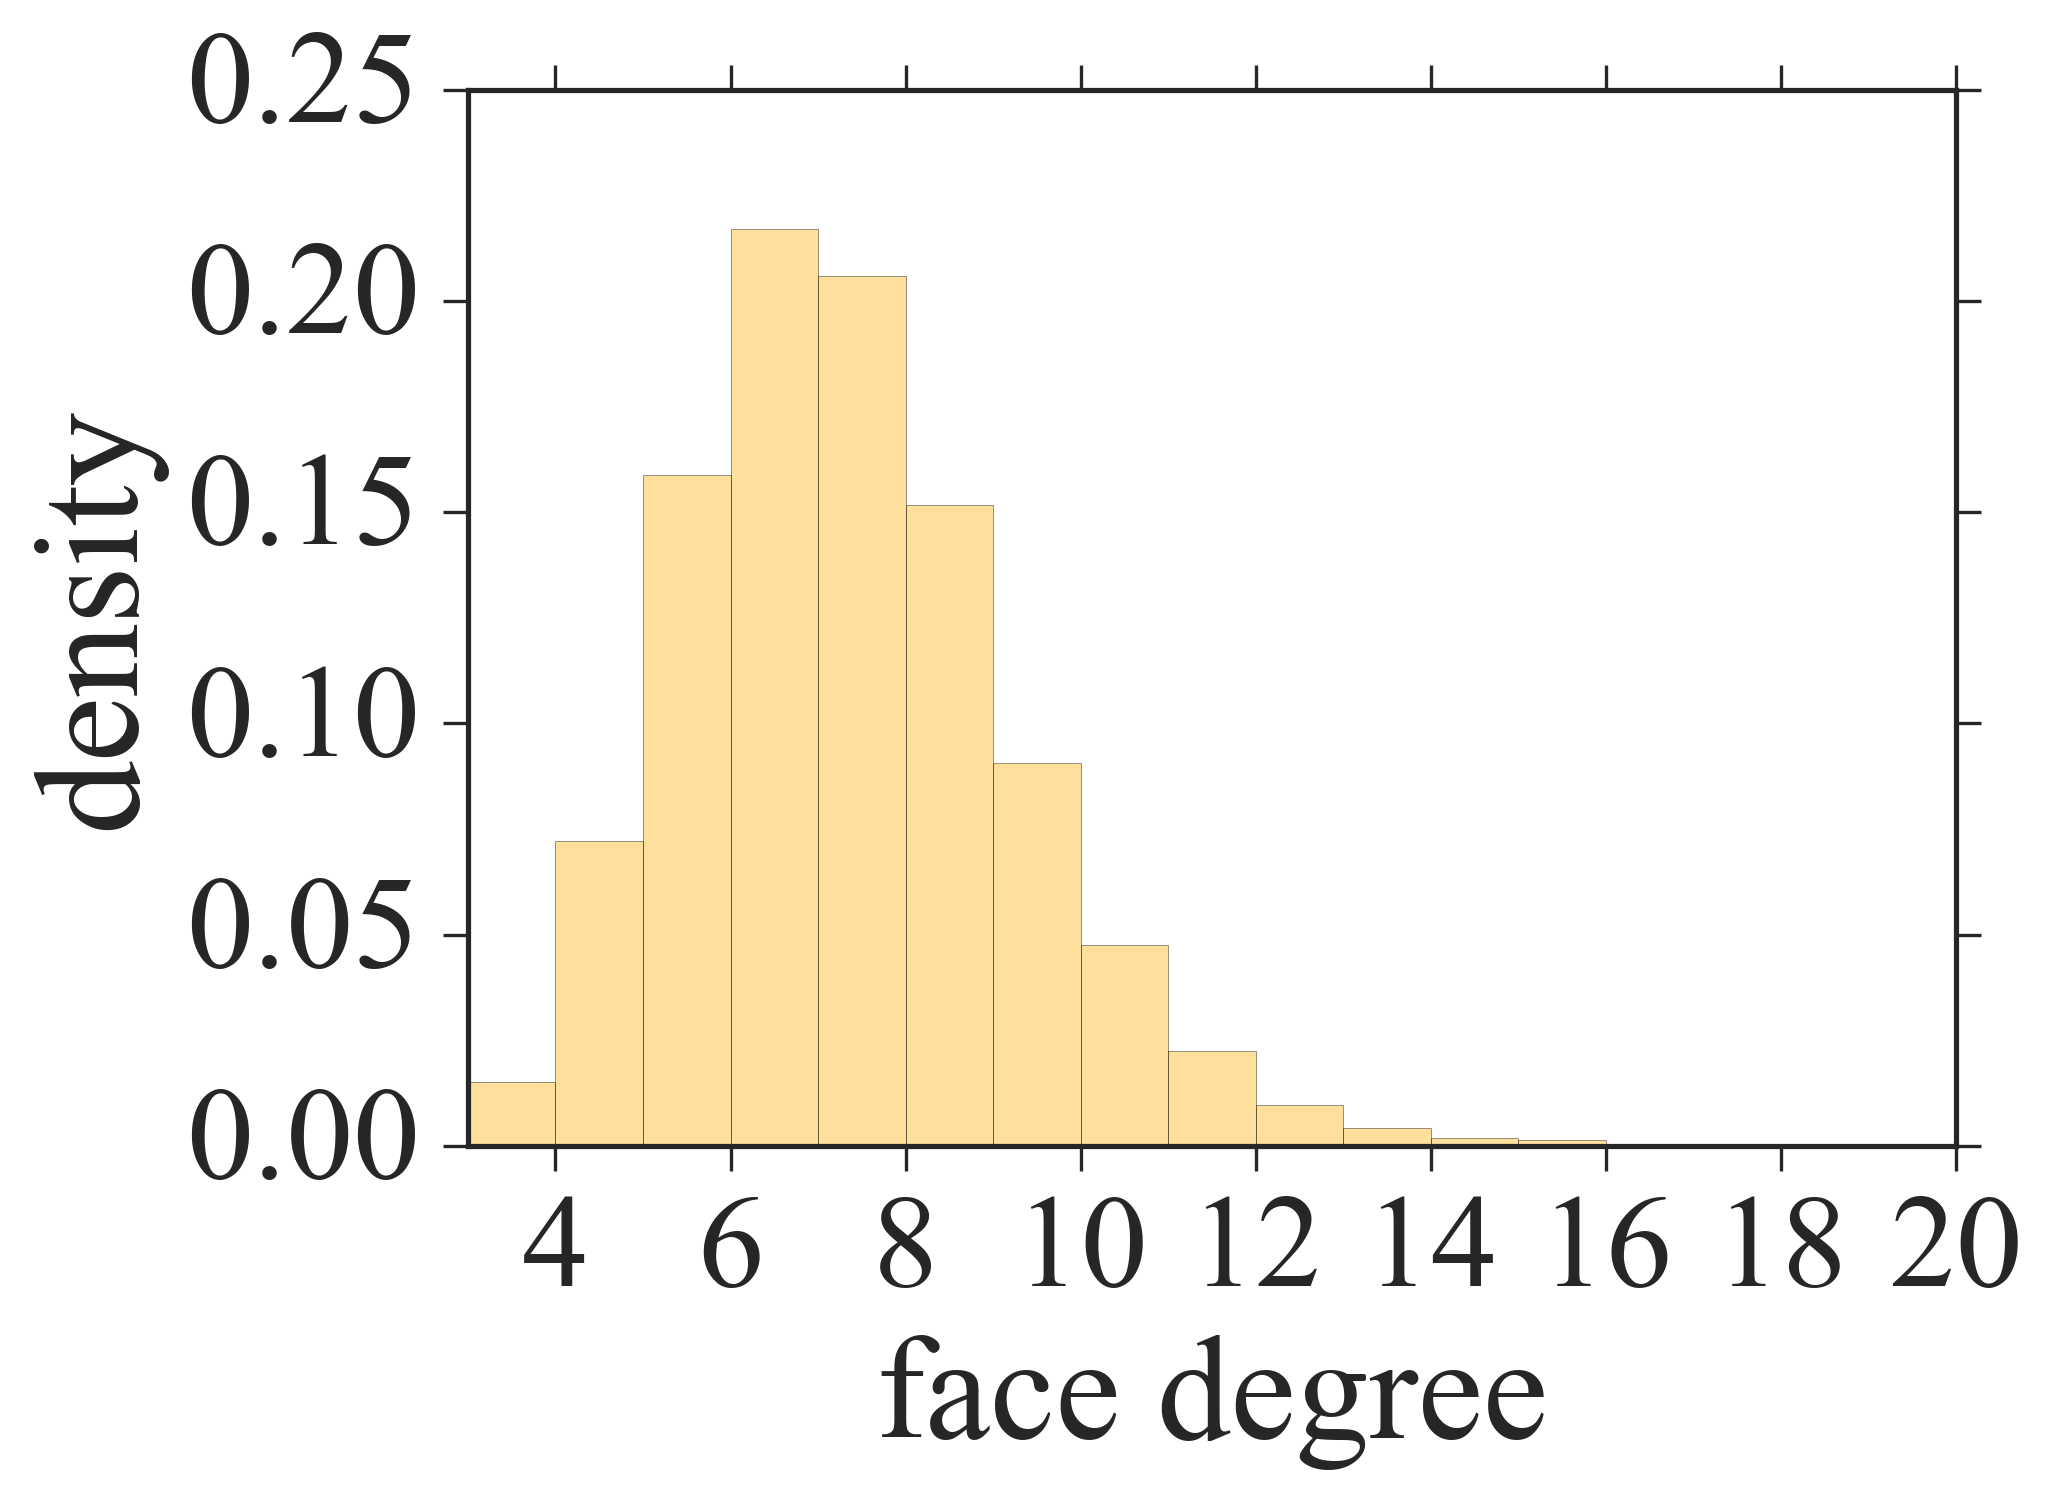
\includegraphics[width=0.55\textwidth]{face_area/face_degree_and_area_cummulative.png}
			\caption[Face degree weighted by face area]{Global cumulative histogram of face degree weighted by face area. The area under the histogram, which is normalized to one, corresponds to the sum of face areas across all observed faces,\ie the total area covered by $1998$ \P graphs.}
			\label{fig:face_degree_per_area}
		\end{figure}

		Let us now move on to the empirical distributions of the circumferences of faces. The cumulative face circumference distribution for \series{35} is given in \Fref{fig:face_length_fit_histogram}. Here, goodness-of-fit plots indicate that a gamma distribution is clearly superior to other candidate fits, see \Fref{fig:sup::face_length_goodness}. Surprisingly, this is true for all our datasets. \Fref{fig:face_length_fit_parameters} shows the time development of rate and shape, indicating that the distribution is shifting towards faces of larger circumference. This time development can be seen for a significant fraction of the available data.

		\begin{figure}
			\centering
			\subfloat[][]{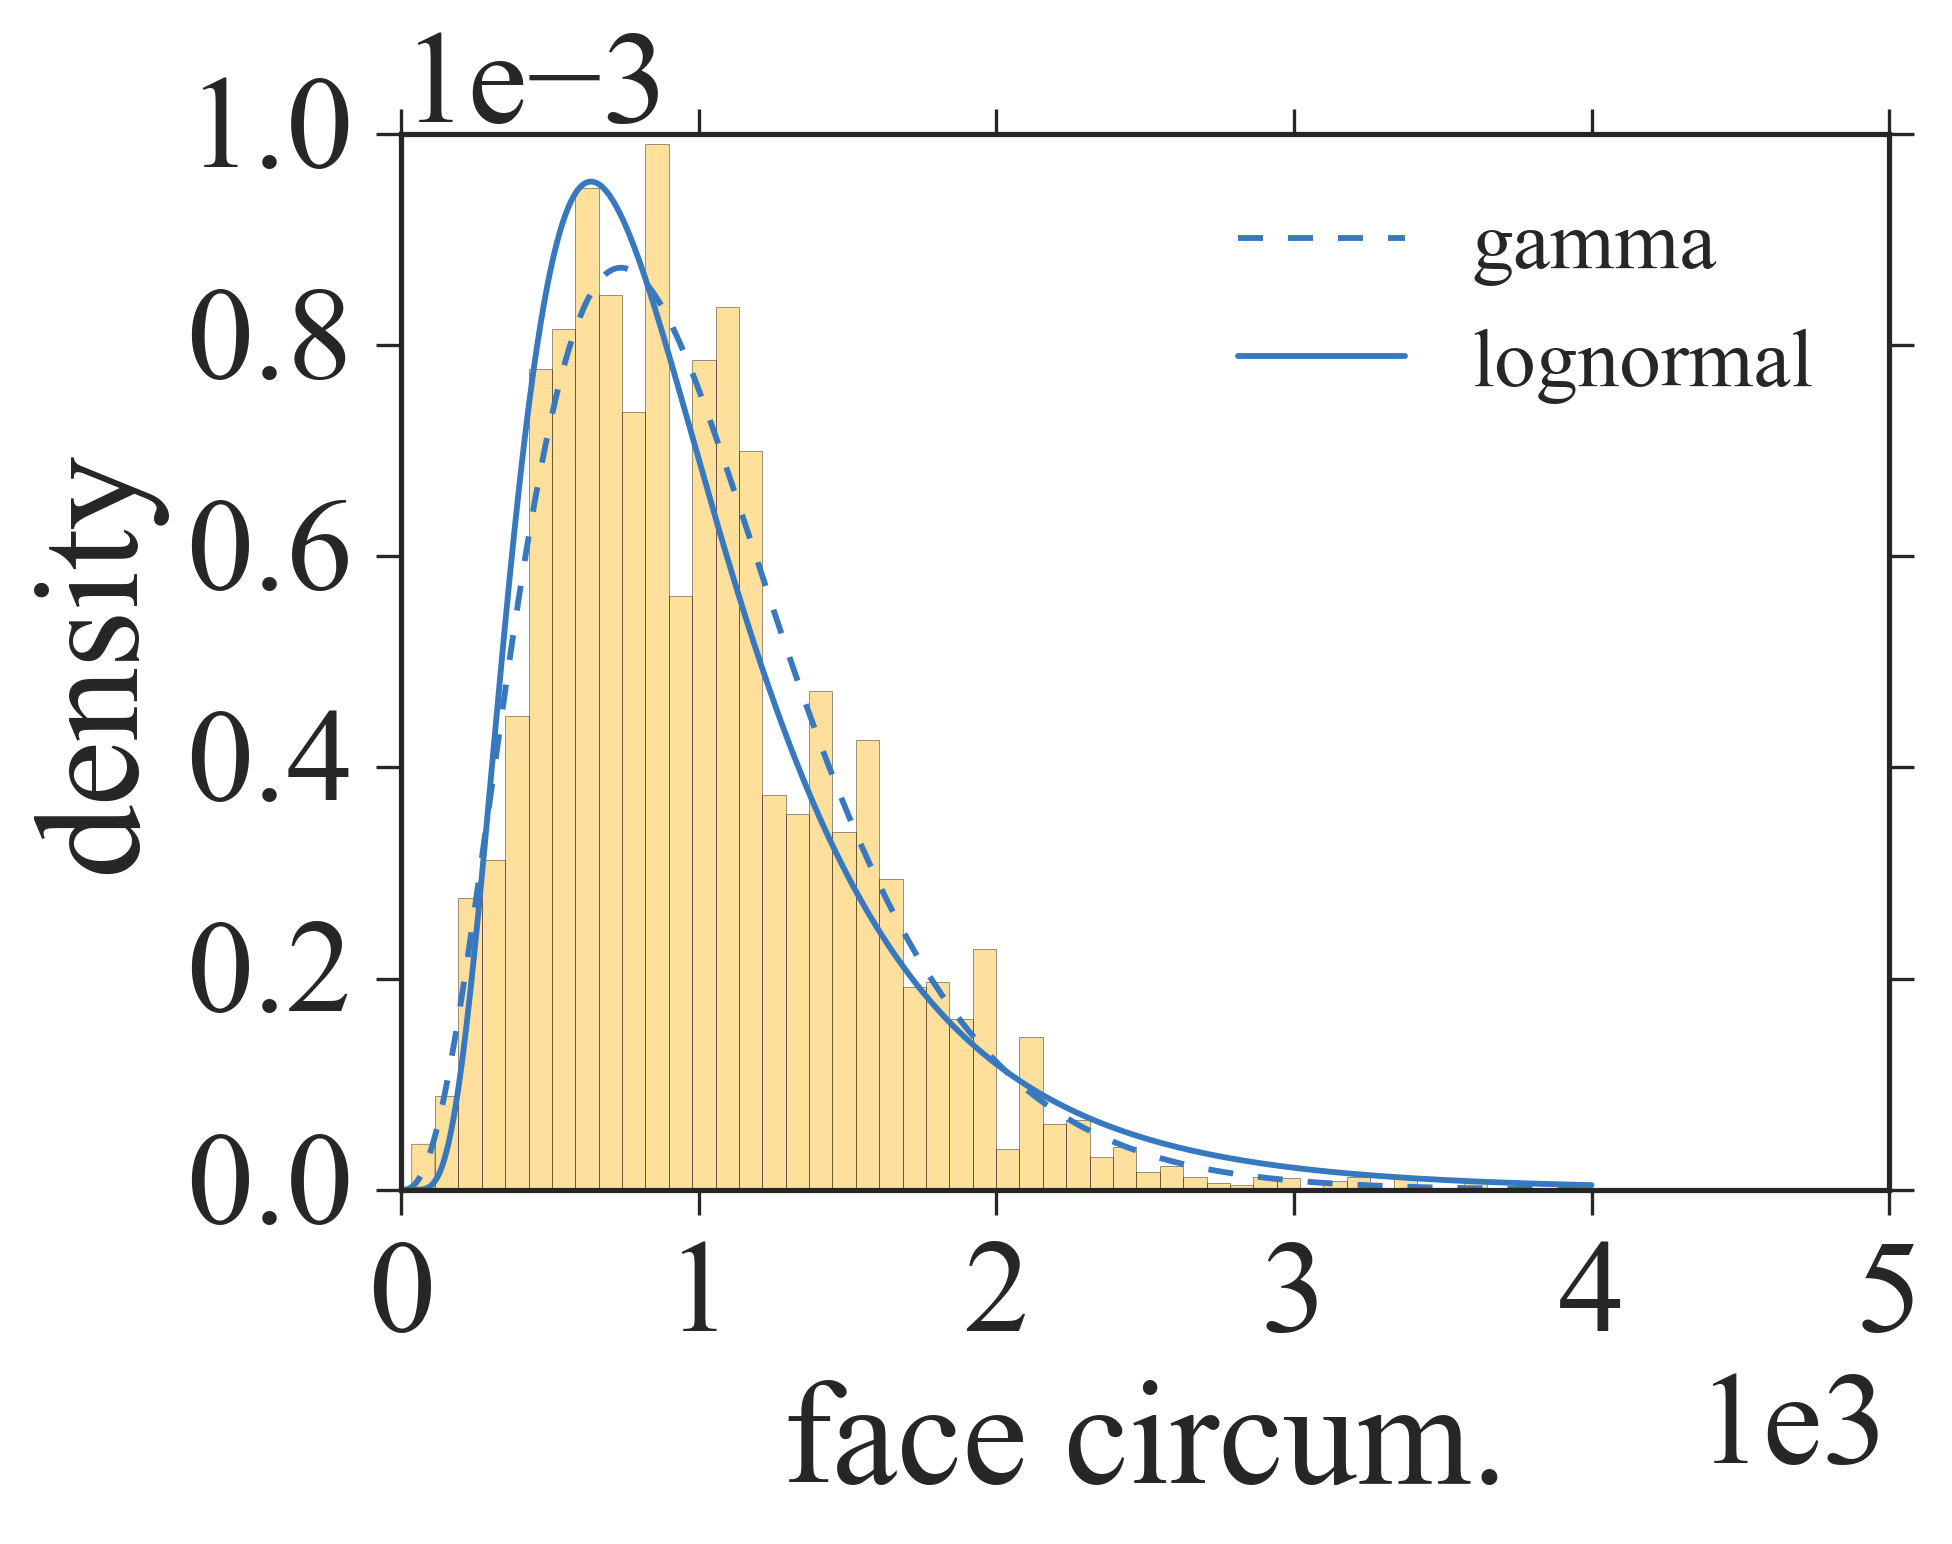
\includegraphics[width=\twoimageswide,keepaspectratio]{face_length/face_circum_motion35.png}
			\label{fig:face_length_fit_histogram}}\qquad
			\subfloat[][]{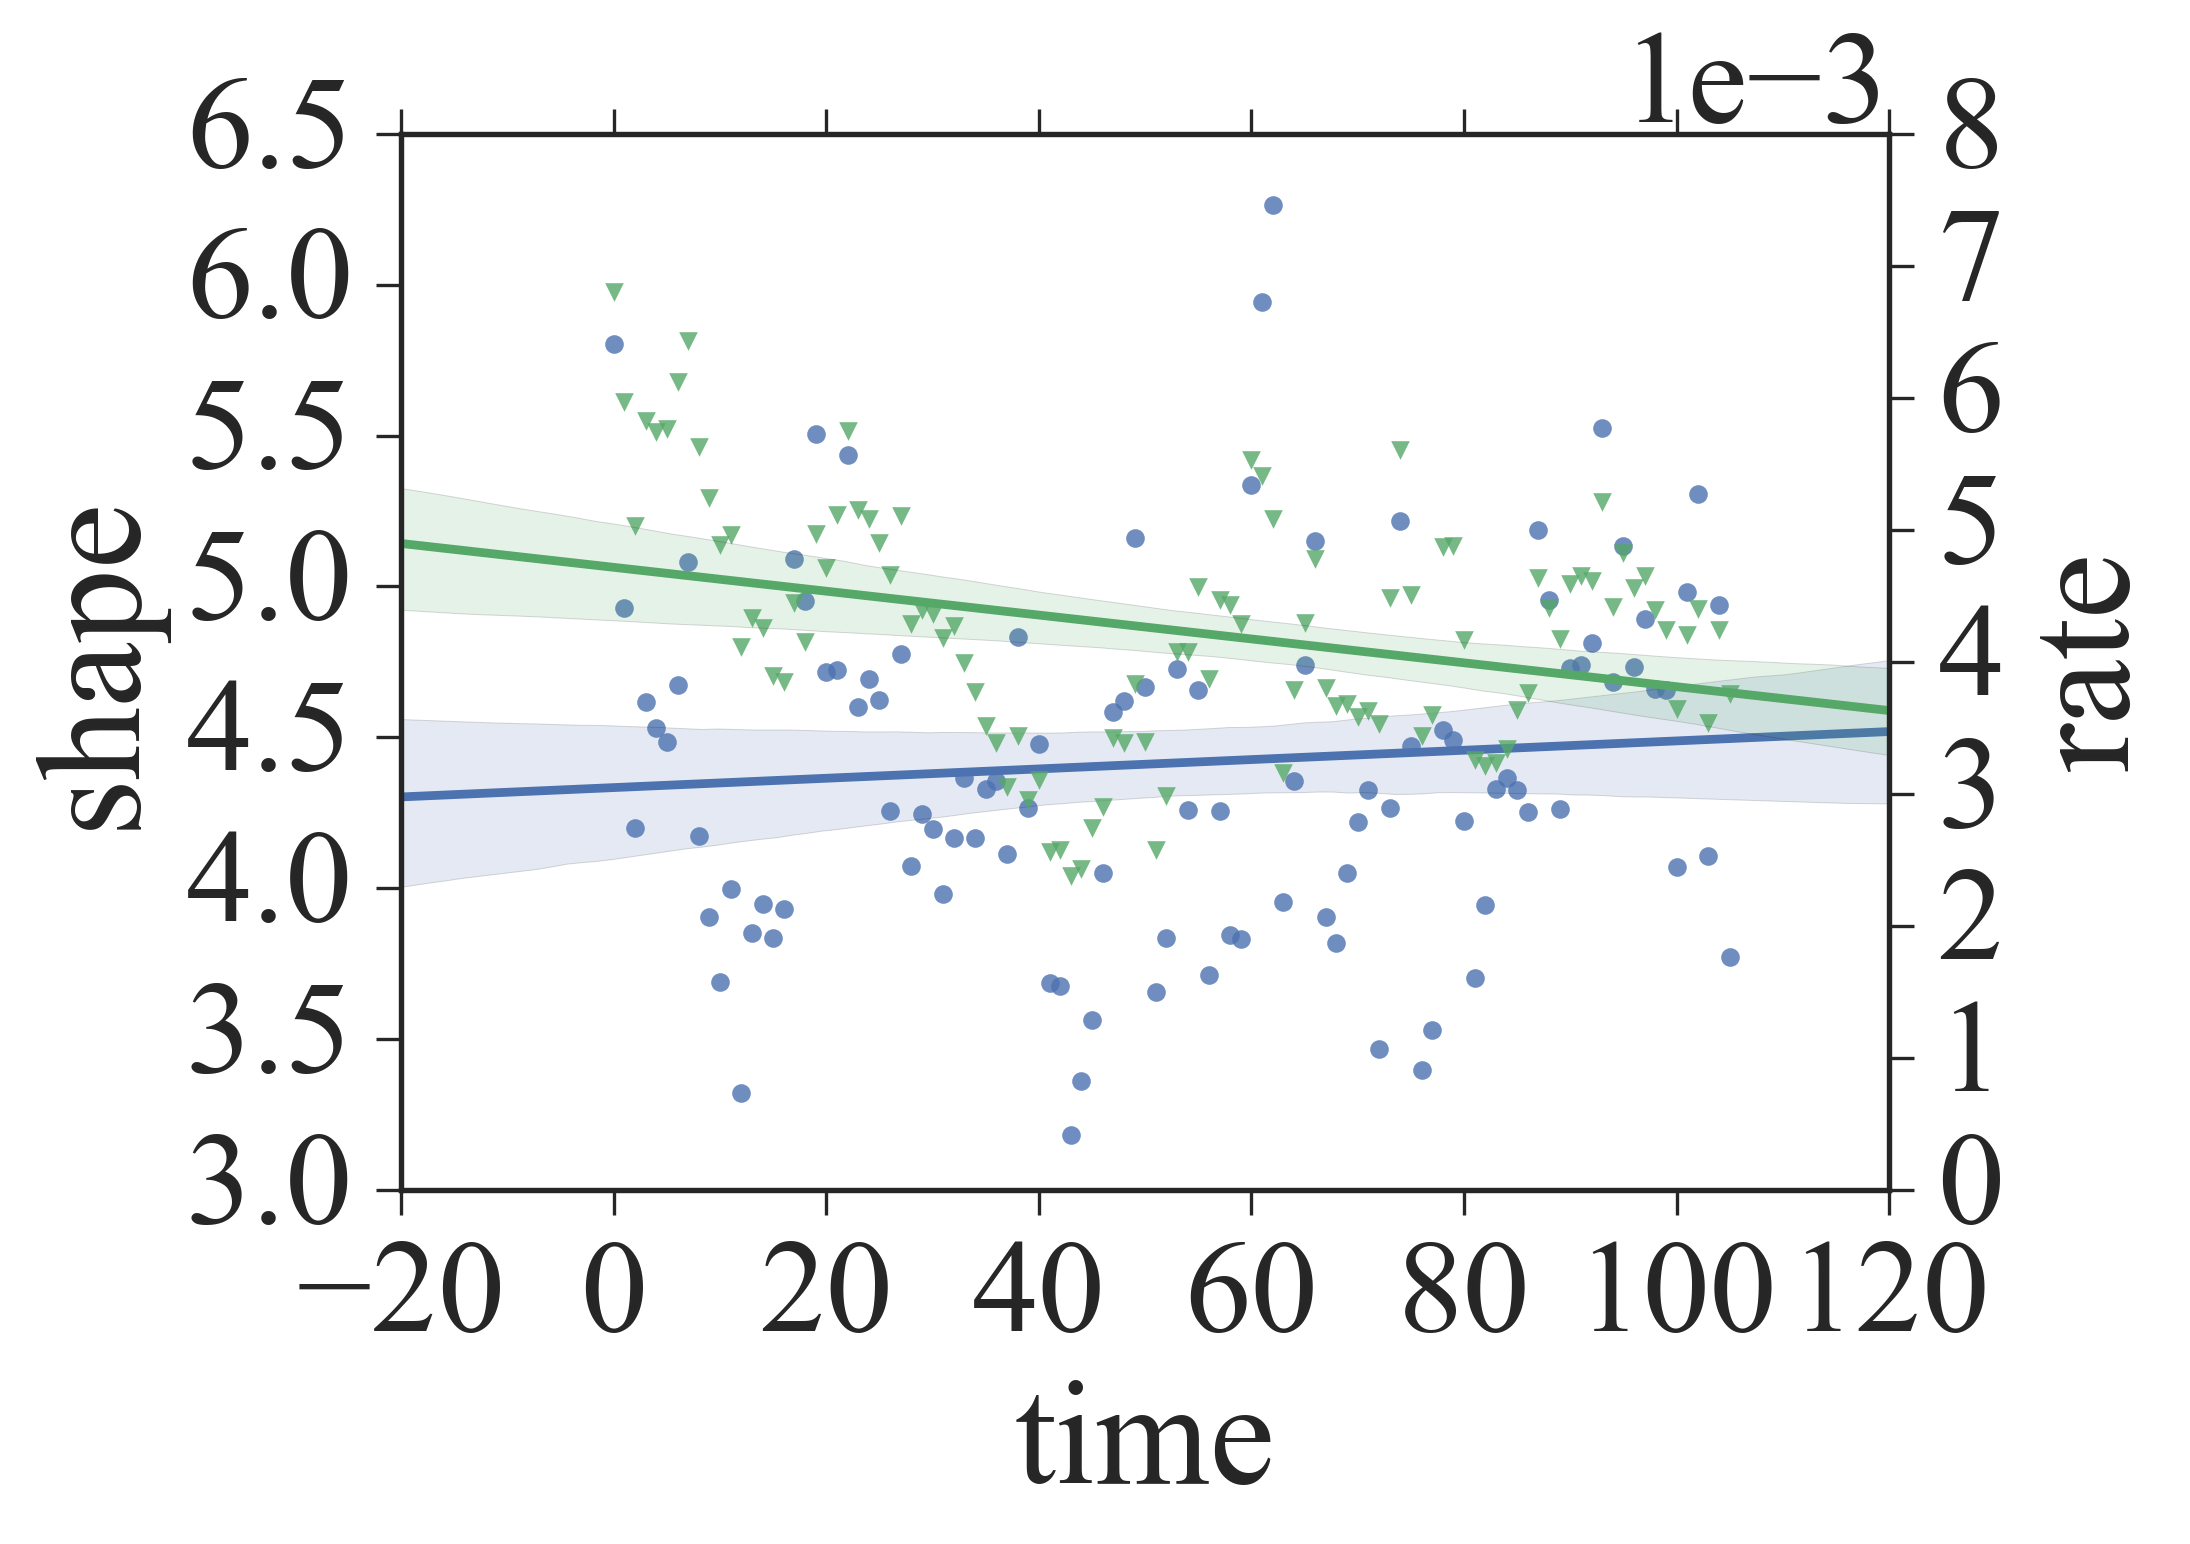
\includegraphics[width=\twoimageswide,keepaspectratio]{face_length/face_length_gamma_fit_parameters_together_motion35.png}
			\label{fig:face_length_fit_parameters}}

			\caption[Face circumference distribution]{(a): Cumulative empirical face circumference distribution for \series{35}. Candidate gamma and log normal fits are shown. Abscissa in units of \si{\pixel}. (b): Gamma fit parameters shape (blue circles) and rate (green triangles) as a function of time for the same series. Linear fits are shown to guide the eye. Abscissa in units of \SI{120}{\second}.}
			\label{fig:face_length_fit}
		\end{figure}

		Finally, a global impression of the obtained fit parameters is given in \Fref{fig:face_length_kde}. Since the shape values are larger than $1$, we may obtain the value of the mode of the distribution associated with the global maximum of the density to be~\SI{627.105}{\pixel}.

		\begin{figure}[!htbp]
			\centering
				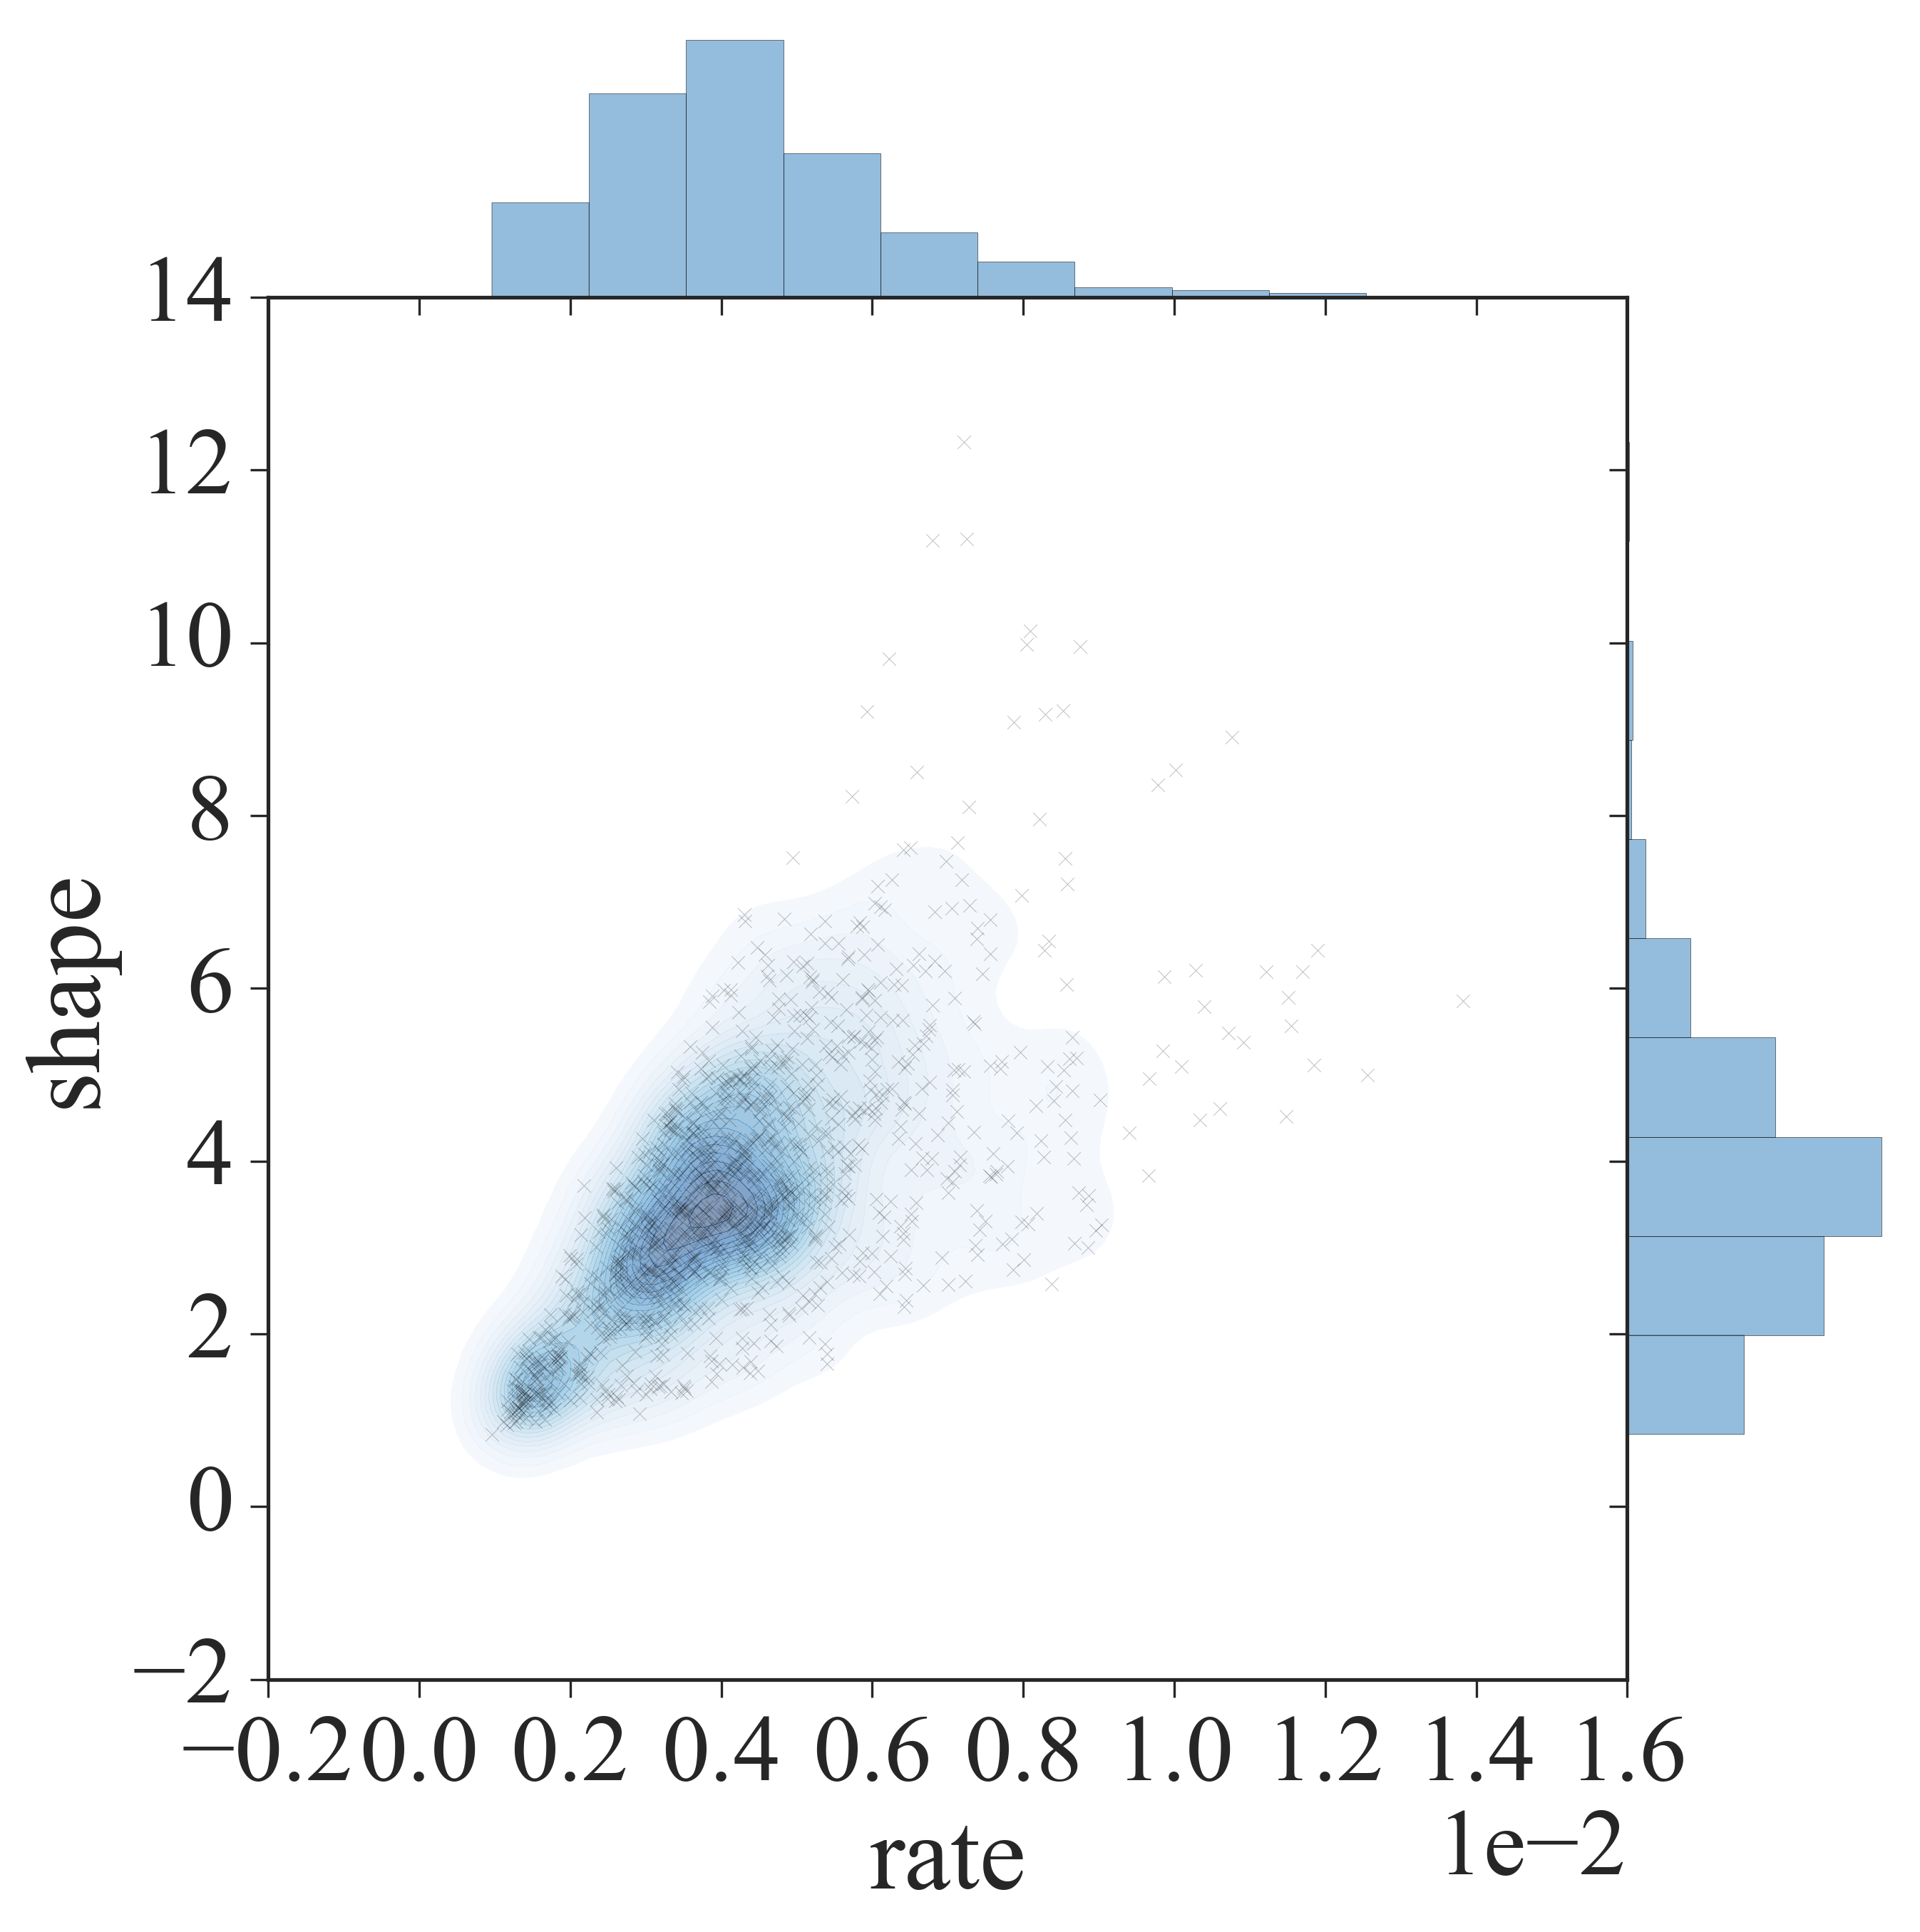
\includegraphics[width=0.75\textwidth]{face_length/face_length_gamma_fit_rate_shape_scatter_cummulative.png}
			\caption[Face circumference distribution - Fit parameter densities]{Scatter-plot and kernel density estimates of shape $s$ and rate $r$ for gamma fits of the empirical face circumference using the entire dataset. The global maximum of the density is located at $s \approx 3.4247$ and $r \approx 3.8665 \times 10^{-3}$.}
			\label{fig:face_length_kde}
		\end{figure}

		Let us complete our report on face properties by characterizing the geometric shape of the faces observed in \P. In particular we want to quantify the resemblance between a face of degree $k$ and a regular polygon consisting of $k$ edges. We do so by defining the dimensionless \emph{roundness} $r(f)$ for any face $f$ as

		\begin{equation}
			 r(f) = \frac{4 \pi A(f)}{C(f)^2}\,,
		\end{equation}
		where $A(f)$ and $C(f)$ denote face area and face circumference respectively. For $k \to \infty$, we have $r(f) = 1$ if $f$ forms a circle, and $0 < r < 1$ if $f$ has any other shape. The closer the polygon defined by $f$ is to a circle, the closer $r$ is to $1$. To obtain an equivalent statement for faces of finite $k$ we need to normalize $r(f)$ with respect to $k$. The normalization factor $r_{max}(k)$ is defined as the roundness of a regular polygon with $k$ edges. It is given by

		\begin{equation}
			r_{max}(k) = \frac{\pi}{k} (tan(\frac{\pi}{k}))^{-1}\,.
		\end{equation}

		Hence, we obtain the \emph{normalized roundness} of a face $f$ of degree $k$ as

		\begin{equation}
			R(f,k) = \frac{r(f)}{r_{max}(k)}\,.
		\end{equation}

		Thus for any $k$ it holds that, the closer $R(f,k)$ is to $1$, the closer a face $f$ of degree $k$ is to being a regular polygon consisting of $k$ edges. 

		With this definition we give the empirical distribution of the $R(f,k)$ for all faces in \series{35} in \Fref{fig:face_roundness}. The distribution is sharply concentrated around $0.8513 \pm 0.0077$ indicating a tendency for the faces of the underlying graphs to approach regular polygons. A value of $0.8532 \pm 0.0205$ is found when the entire dataset is considered. \Fref{fig:face_roundness_evolution} indicates that the mode of the roundness shows only small variations in time for \series{35}. The fact that this behavior is consistent across all datasets makes the roundness a very distinct and robust quantity describing the face structure of \P graphs.

		\begin{figure}
			\centering
			\subfloat[][]{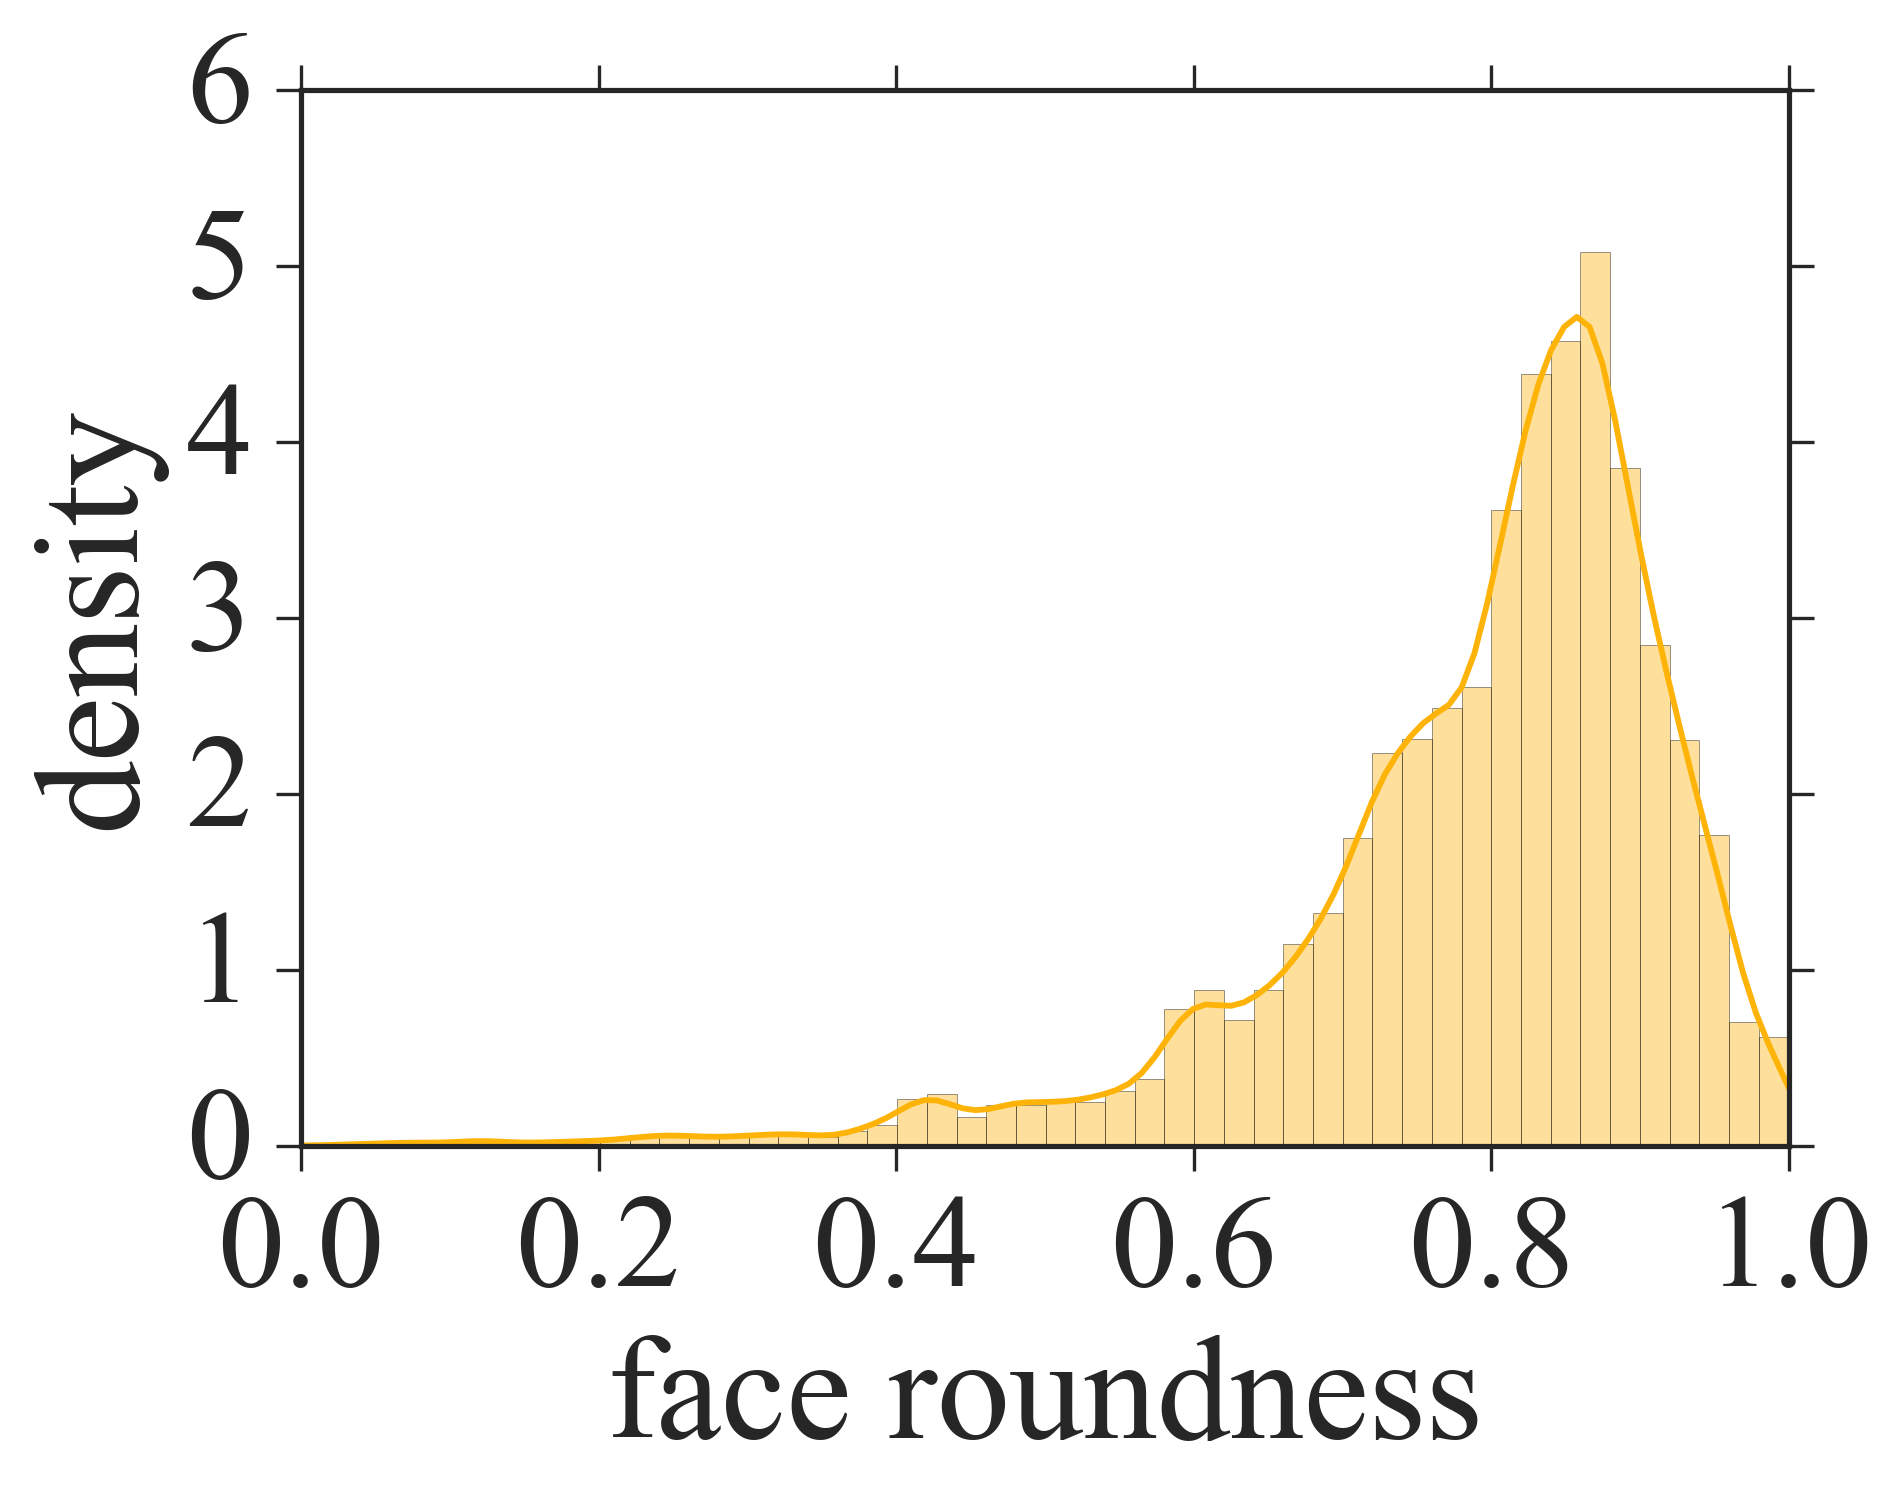
\includegraphics[width=\twoimageswide,keepaspectratio]{face_roundness/face_roundness_motion35.png}
			\label{fig:face_roundness}}\qquad
			\subfloat[][]{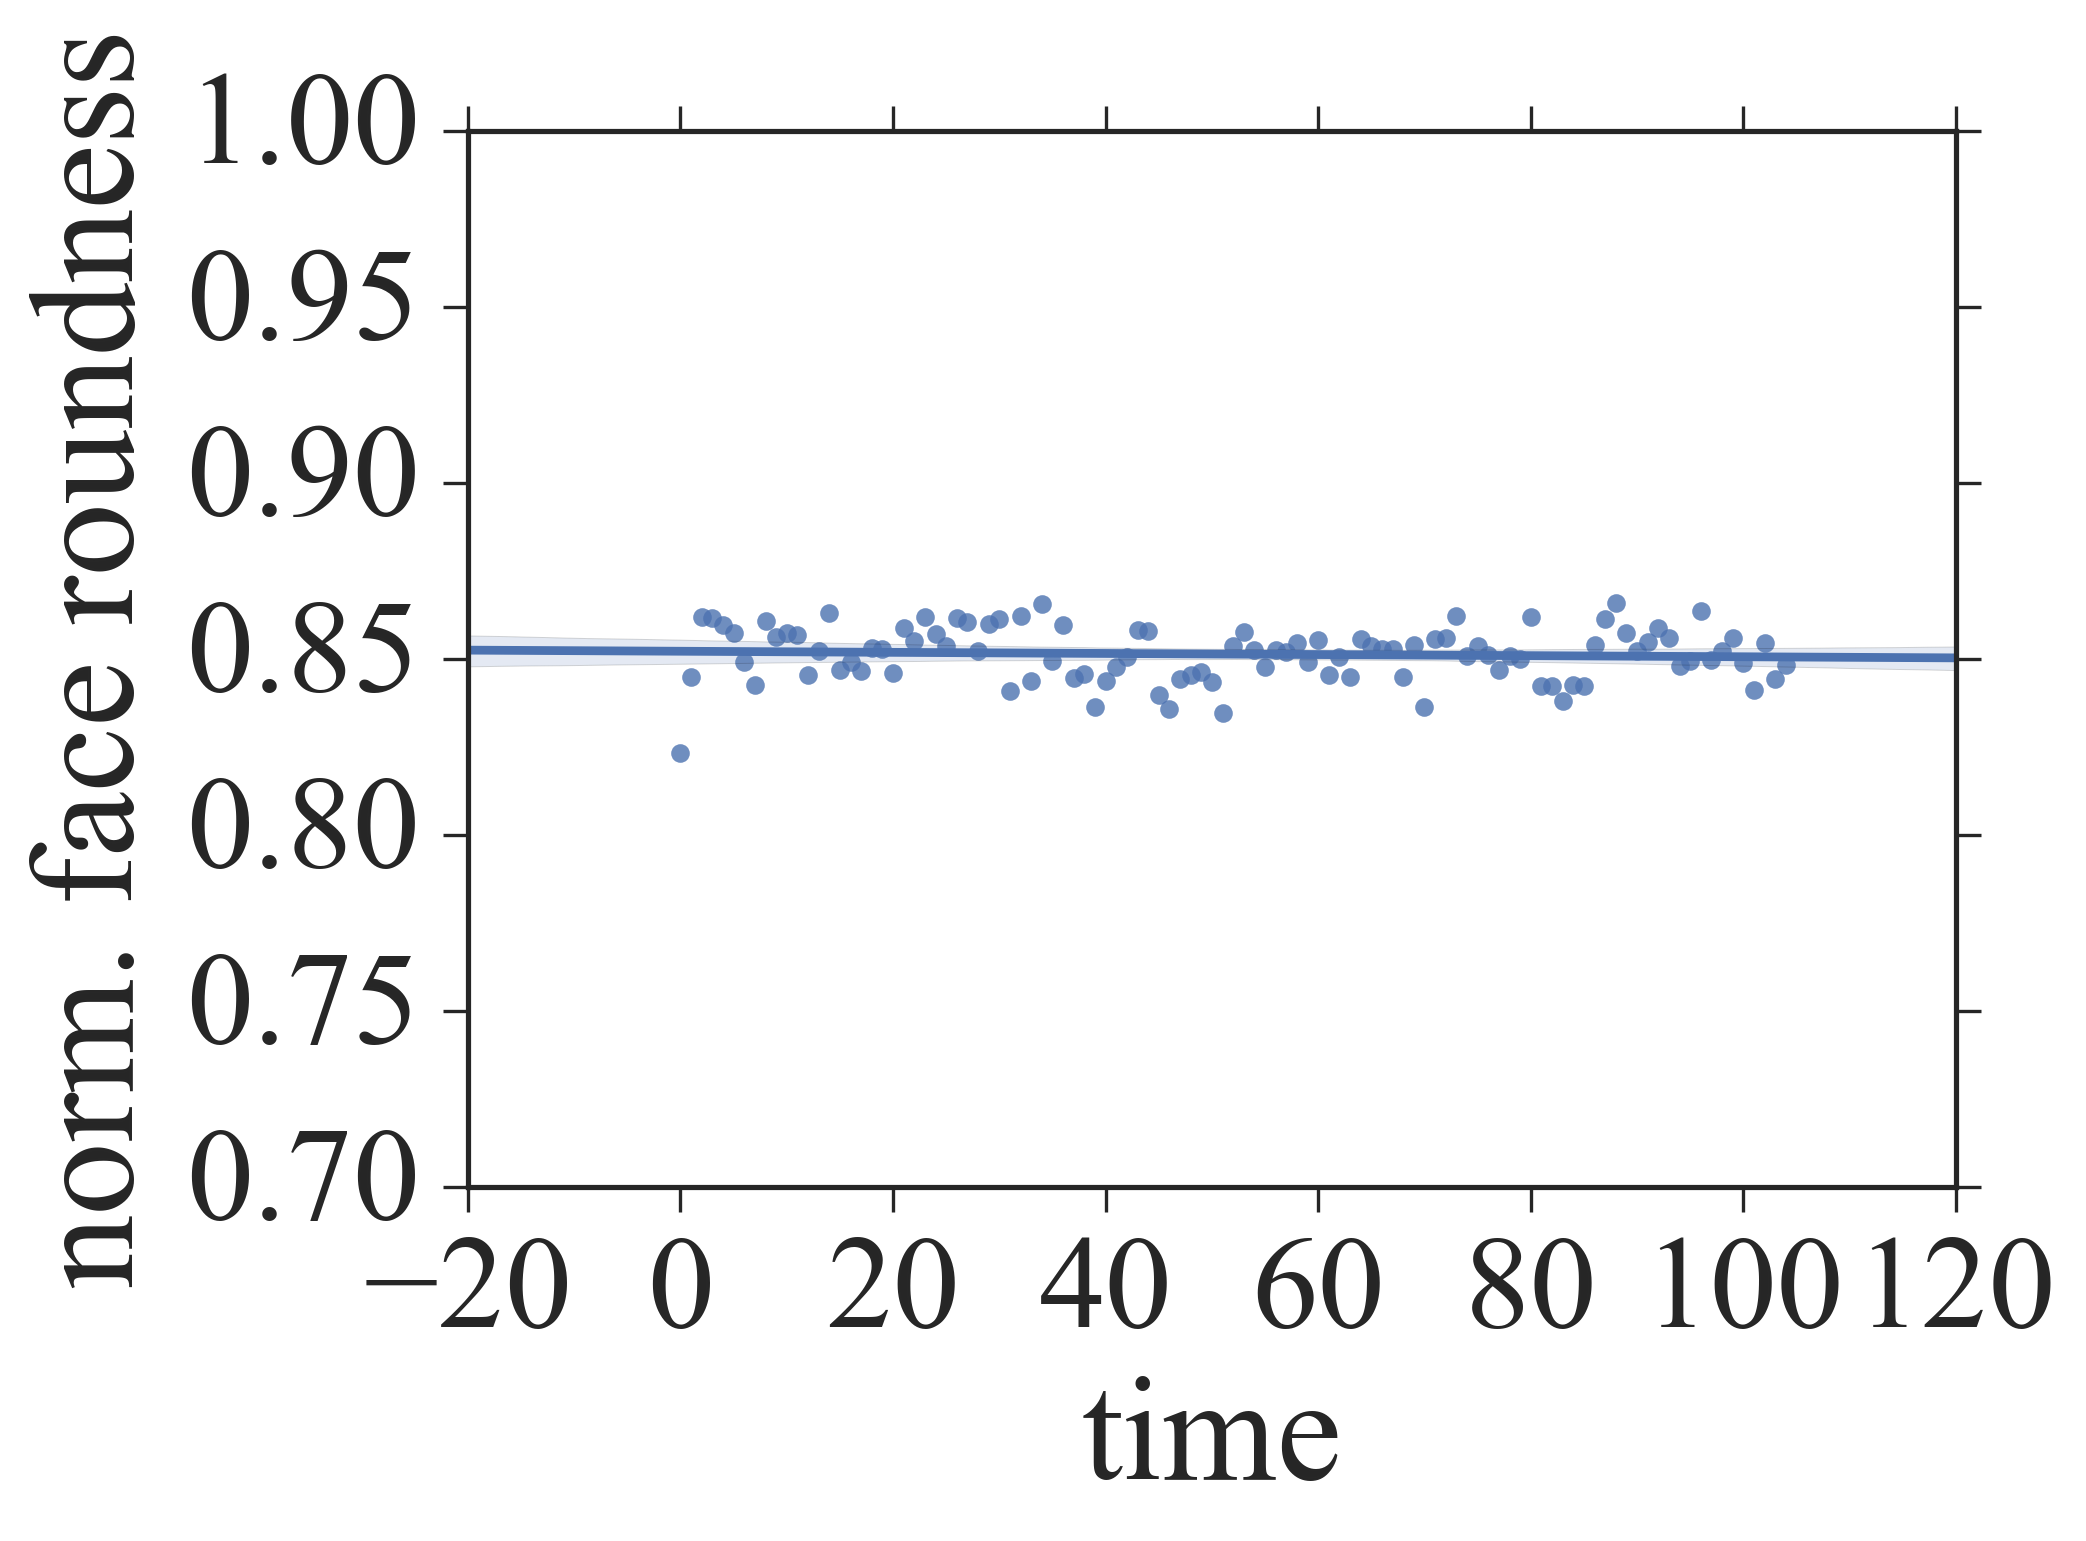
\includegraphics[width=\twoimageswide,keepaspectratio]{face_roundness/face_roundness_mode_motion35.png}
			\label{fig:face_roundness_evolution}}

			\caption[Face roundness distribution]{(a) Cumulative normalized face roundness distribution for \series{35}. The kernel density estimation of the cumulative distribution is show as a solid line. The value of the abscissa at the maximum of the KDE serves as an estimate for the mode of the underlying unknown theoretical distribution. (b) The development of the estimates of the mode for the individual networks of \series{35}. Abscissa in units of \SI{120}{\second}.}
		\end{figure}

		It is interesting to investigate how the roundness is connected to the degree of the faces under consideration. \Fref{fig:face_roundness_per_degree} shows the roundness values averaged over classes of faces that have the same degree. We find that the roundness steadily increases with $k$ to reach a maximum of $0.8206 \pm 0.0014$ for $k=7$. After the maximum is attained the roundness falls off again, albeit slightly. We may also ask which class of faces contributes the most to the global sum of observed roundness values. \Fref{fig:face_roundness_per_time_degree} shows the histogram of face degrees weighted by face roundness. It indicates that faces of degree  $4,5$ and $6$ account for the majority of the global sum of roundness. Since these faces form a large fraction of all available faces, we can now quantify the degree to which \P networks are formed by components that resemble regular polygons.

		\begin{figure}
			\centering
			\subfloat[][]{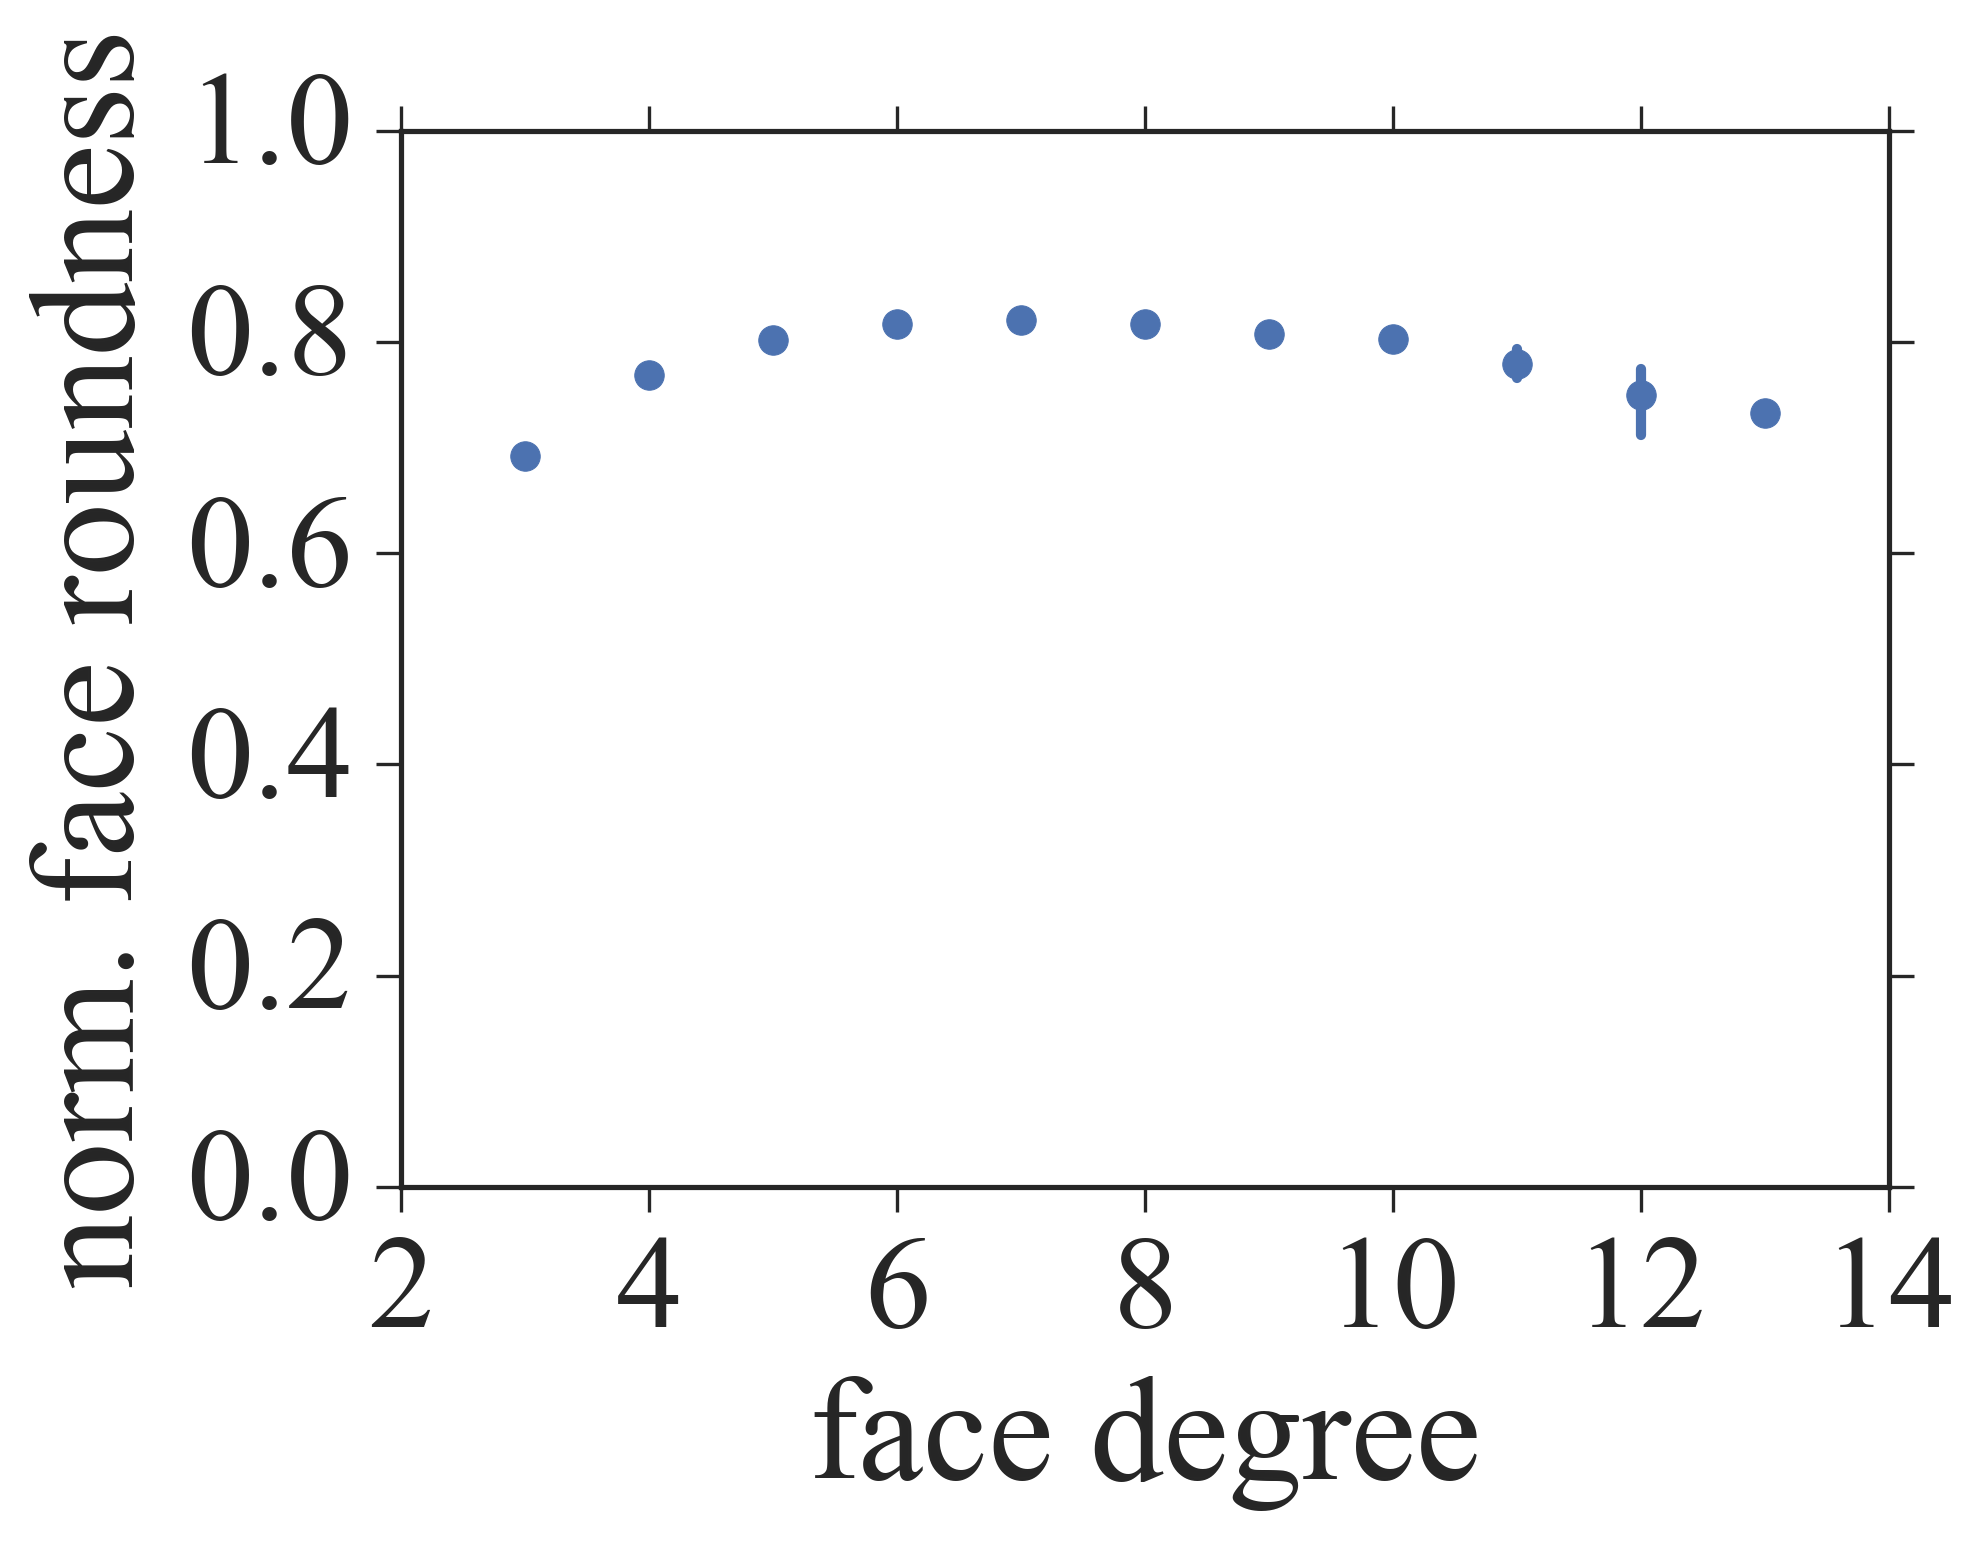
\includegraphics[width=\twoimageswide]{face_roundness/face_roundness_per_face_cummulative.png}
			\label{fig:face_roundness_per_degree}}\qquad
			\subfloat[][]{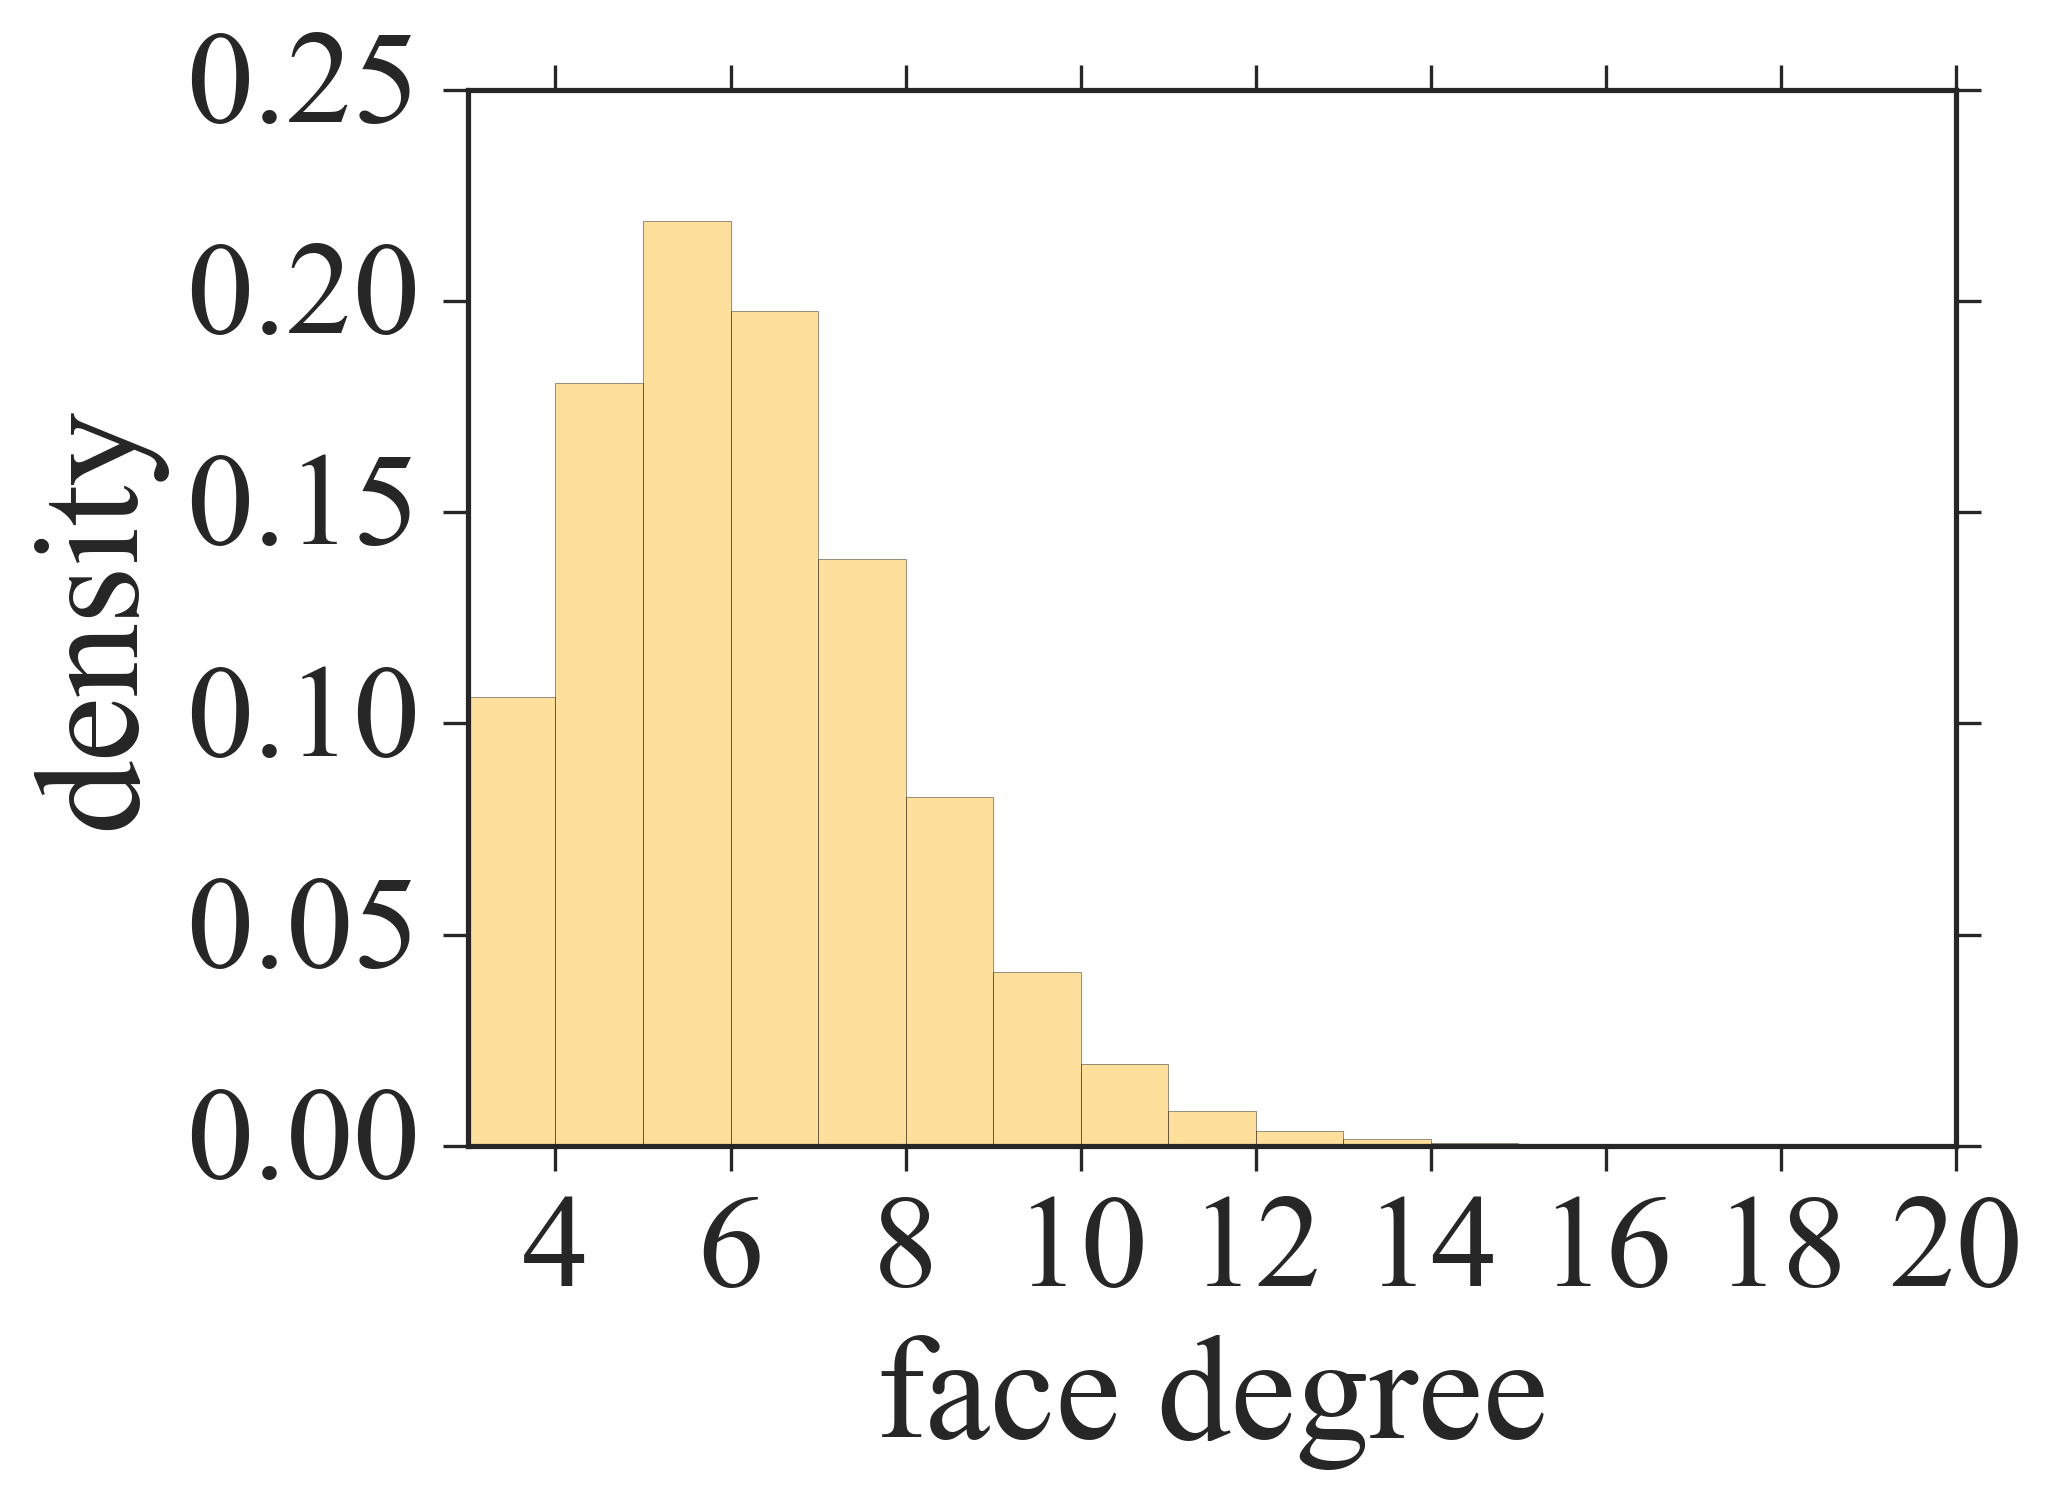
\includegraphics[width=\twoimageswide]{face_roundness/face_degree_and_roundness_cummulative.png}
			\label{fig:face_roundness_per_time_degree}}

			\caption[Average face roundness per face type]{(a) Cumulative normalized face roundness averaged over classes of faces with identical face degree. Classes of size smaller than $30$ are excluded as bootstrapping error-bars ceases to be reliable for small sample sizes. (b) Histogram of face degrees weighted by the associated roundness values. Here the area under the histogram, which is normalized to one, corresponds to the sum of roundness values across all observed faces.}
		\end{figure}

		We stress at this point that looking at roundness numbers by themselves is not very instructive. Their usefulness, however, becomes apparent in combination with other face properties when it comes to comparing \P graphs amongst themselves or with other structures. While the roundness gives a measure of what shapes of faces are present in a graph, face area and circumference add a physical dimension to them. Together with the degree distribution of faces a comprehensive description of the entire network of \P in terms of its basic two dimensional building blocks is available. Since this description can be computed efficiently for any weighted planar graph, a quantitative comparison with other planar networks becomes possible.

	\subsection{Cut Properties}\label{sec:cut_properties}

		In this chapter we study the extend of spatial homogeneity of \P networks with respect to two special directions: First, the direction in which the organism expands, \ie its growth direction and second, the direction perpendicular to it. To do so we use the graph theoretic concept of \emph{cuts}. A cut defines a partition of the nodes of a graph into two disjoint subsets. Furthermore, it determines a \emph{cut-set}, a set of edges with the property that each edge has one endpoint in each of the two node subsets. These are the edges crossing the cut. Since we are interested in the cut-set only, let us refer to it simply as cut from now on. 

		We distinguish vertical and horizontal cuts, which we determine in the following way. First we take the dimensions of the original images containing the graphs of a series. For each series this yields a rectangle of a certain size. Next we partition these rectangles by slicing them into $100$ identical smaller sub-rectangles. Here we distinguish between horizontal and vertical slices. For each image we overlay the resulting horizontal/vertical lines with the graph extracted from the image. Each horizontal/vertical line crosses through a unique set of edges which defines a cut. Thus, for each graph in a series we obtain $100$ equidistant horizontal/vertical cuts. Vertical cuts proceed from left to right, \ie in the direction of growth. Horizontal cuts proceed from top to bottom, \ie perpendicular to the direction of network expansion, see \Fref{fig:sup::physarum_roi}. Since cuts are defined consistently within a series, we may study how interesting cut properties change as we proceed through the cuts. By comparing the two types of cuts we can shed light on structural properties of the network with respect to its growth direction (vertical cuts) or perpendicular to it (horizontal cuts). We define three such properties: the size, the width and the length of a cut. The size of a cut is given by the number of its cut edges. The width of a cut is the sum of the widths of all the edges in the cut while the length of a cut sums over the lengths of the cut edges. 

		We begin by discussing the size of cuts for both horizontal and vertical cuts. \Fref{fig:size_cuts_left} and \Fref{fig:size_cuts_right} give the results for two characteristic data series. For any given cut, the ordinate shows the value of the cut averaged across all graphs in the respective series while the abscissa enumerates the cuts in a sequence of cuts. Both \series{45} and \series{35} exhibit significant fluctuations in the actual cut values. This is to be expected since the network keeps changing as time advances. Linear fits are applied to illustrate trends in the development of the cut values. Looking at \series{45}, it can be seen that, within fluctuations, vertical cut values remain rather stable while horizontal cuts show only a slight tendency to increase in value. The behavior of the cut values of \series{45} indicates that it has a large degree of spatial homogeneity. The situation is different for \series{35} where vertical cuts show a trend to decrease while horizontal cuts tend to increase at the same time. The fact that the behavior of the lengths and widths of cuts closely mirrors the cut sizes, indicates that the properties of the edges that are being cut are homogeneous throughout the network. Differences in cut lengths or widths are predominately due to differences in cut sizes.

		Taking into account the entire data set we find that horizontal cuts remain largely constant, while the vertical cuts frequently show significant changes. The latter include both increasing and decreasing cut values.

		\begin{figure}
			\centering
			\subfloat[][]{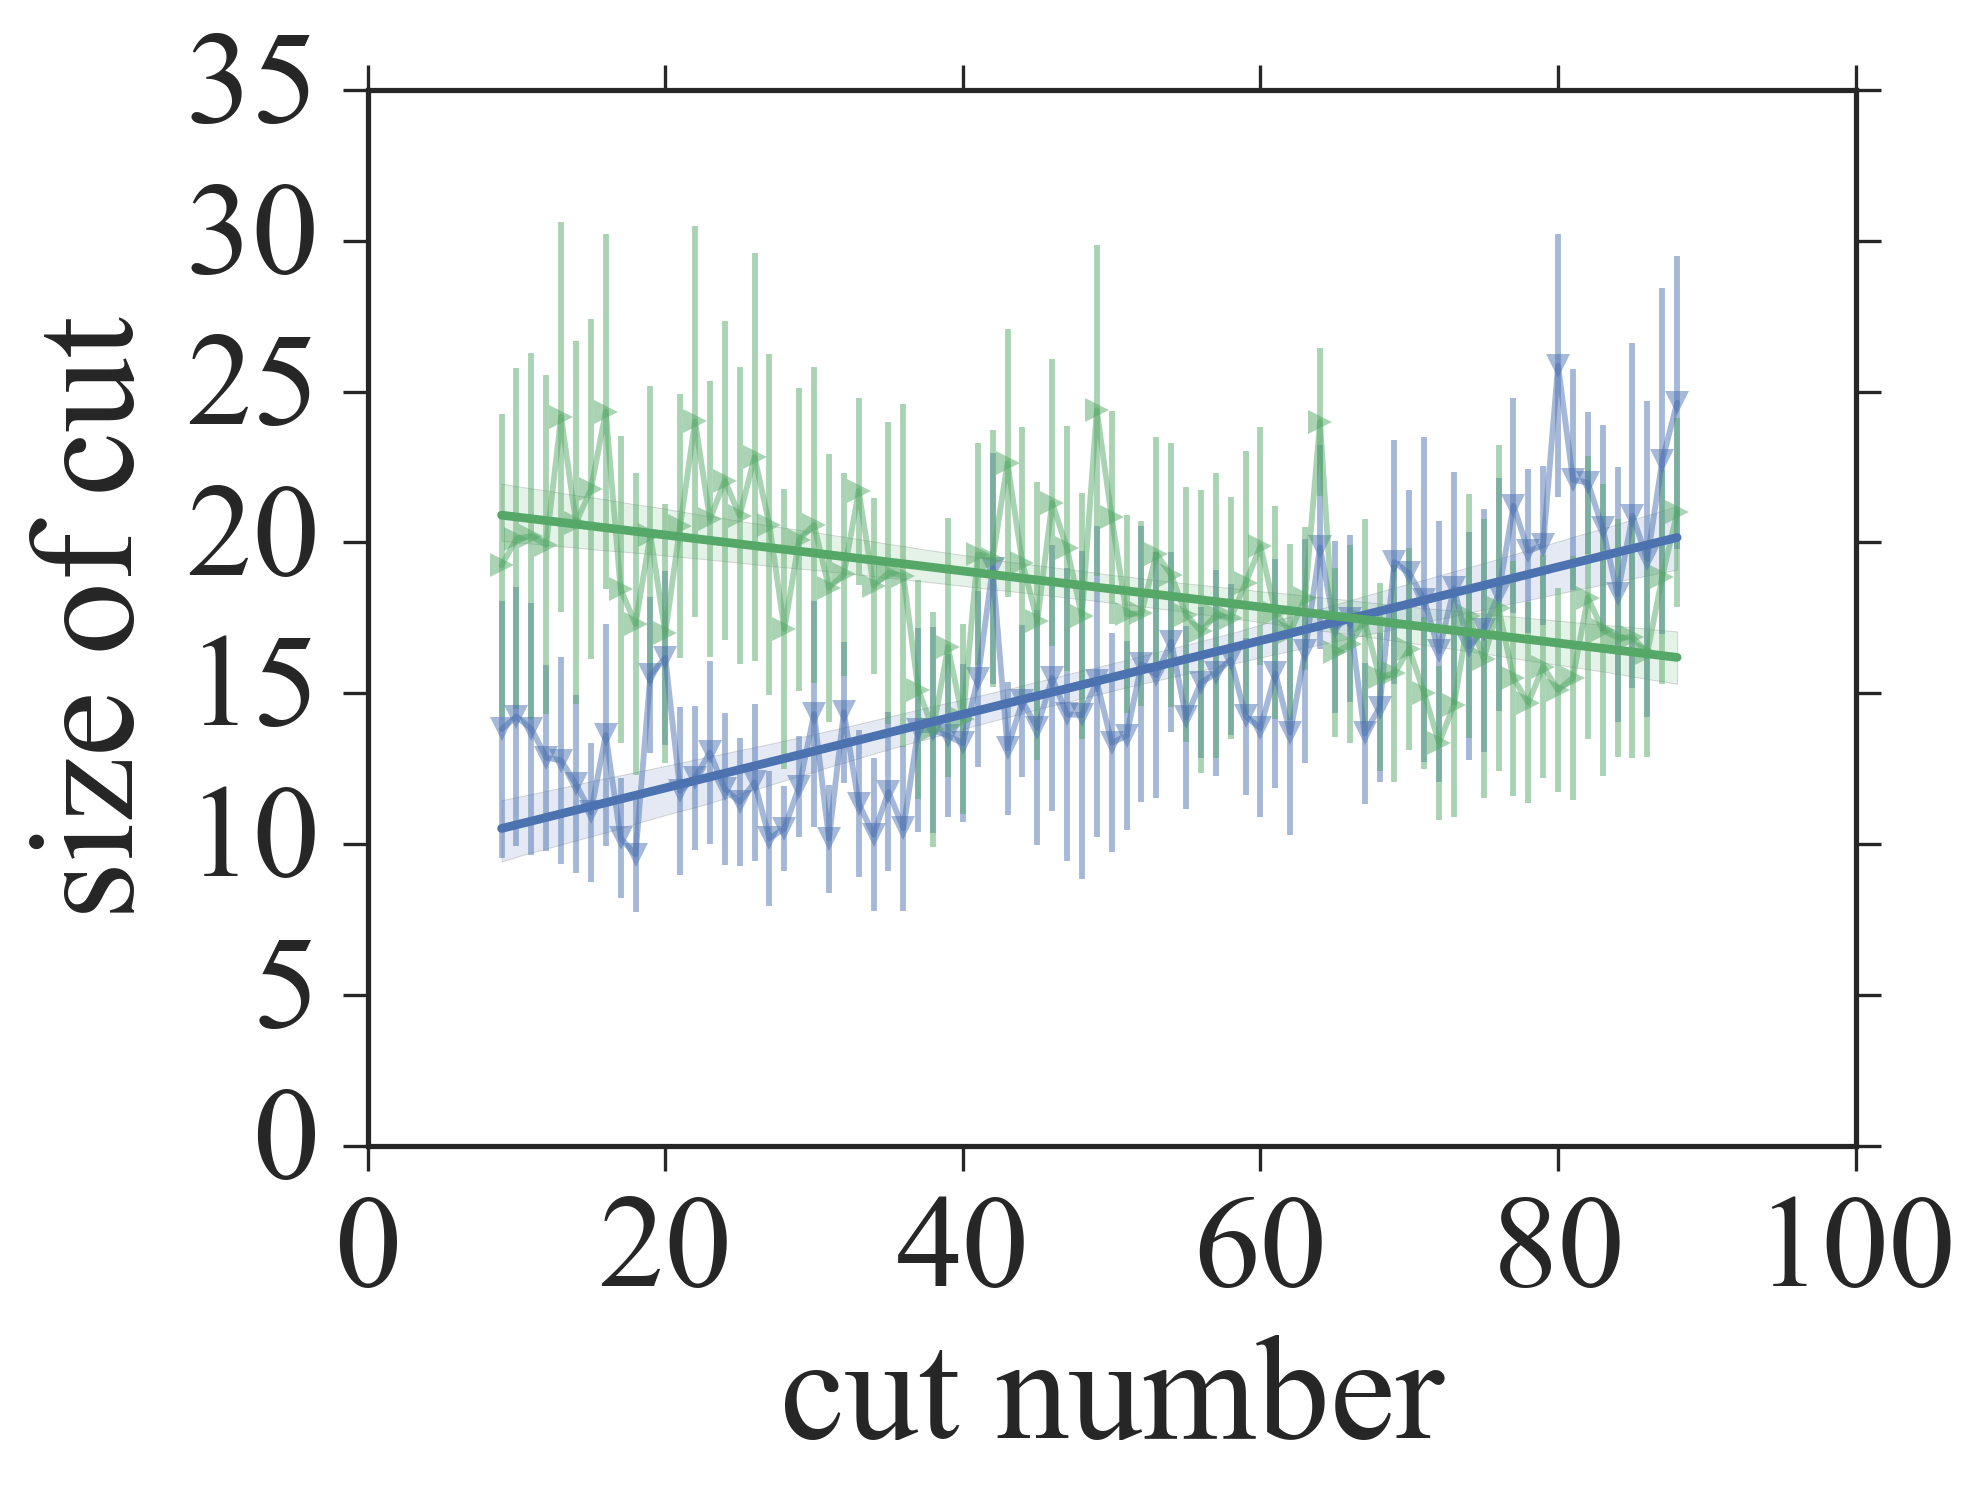
\includegraphics[width=\twoimageswide,keepaspectratio]{cuts/size_cuts_motion35.png}\label{fig:size_cuts_left}}\qquad
			\subfloat[][]{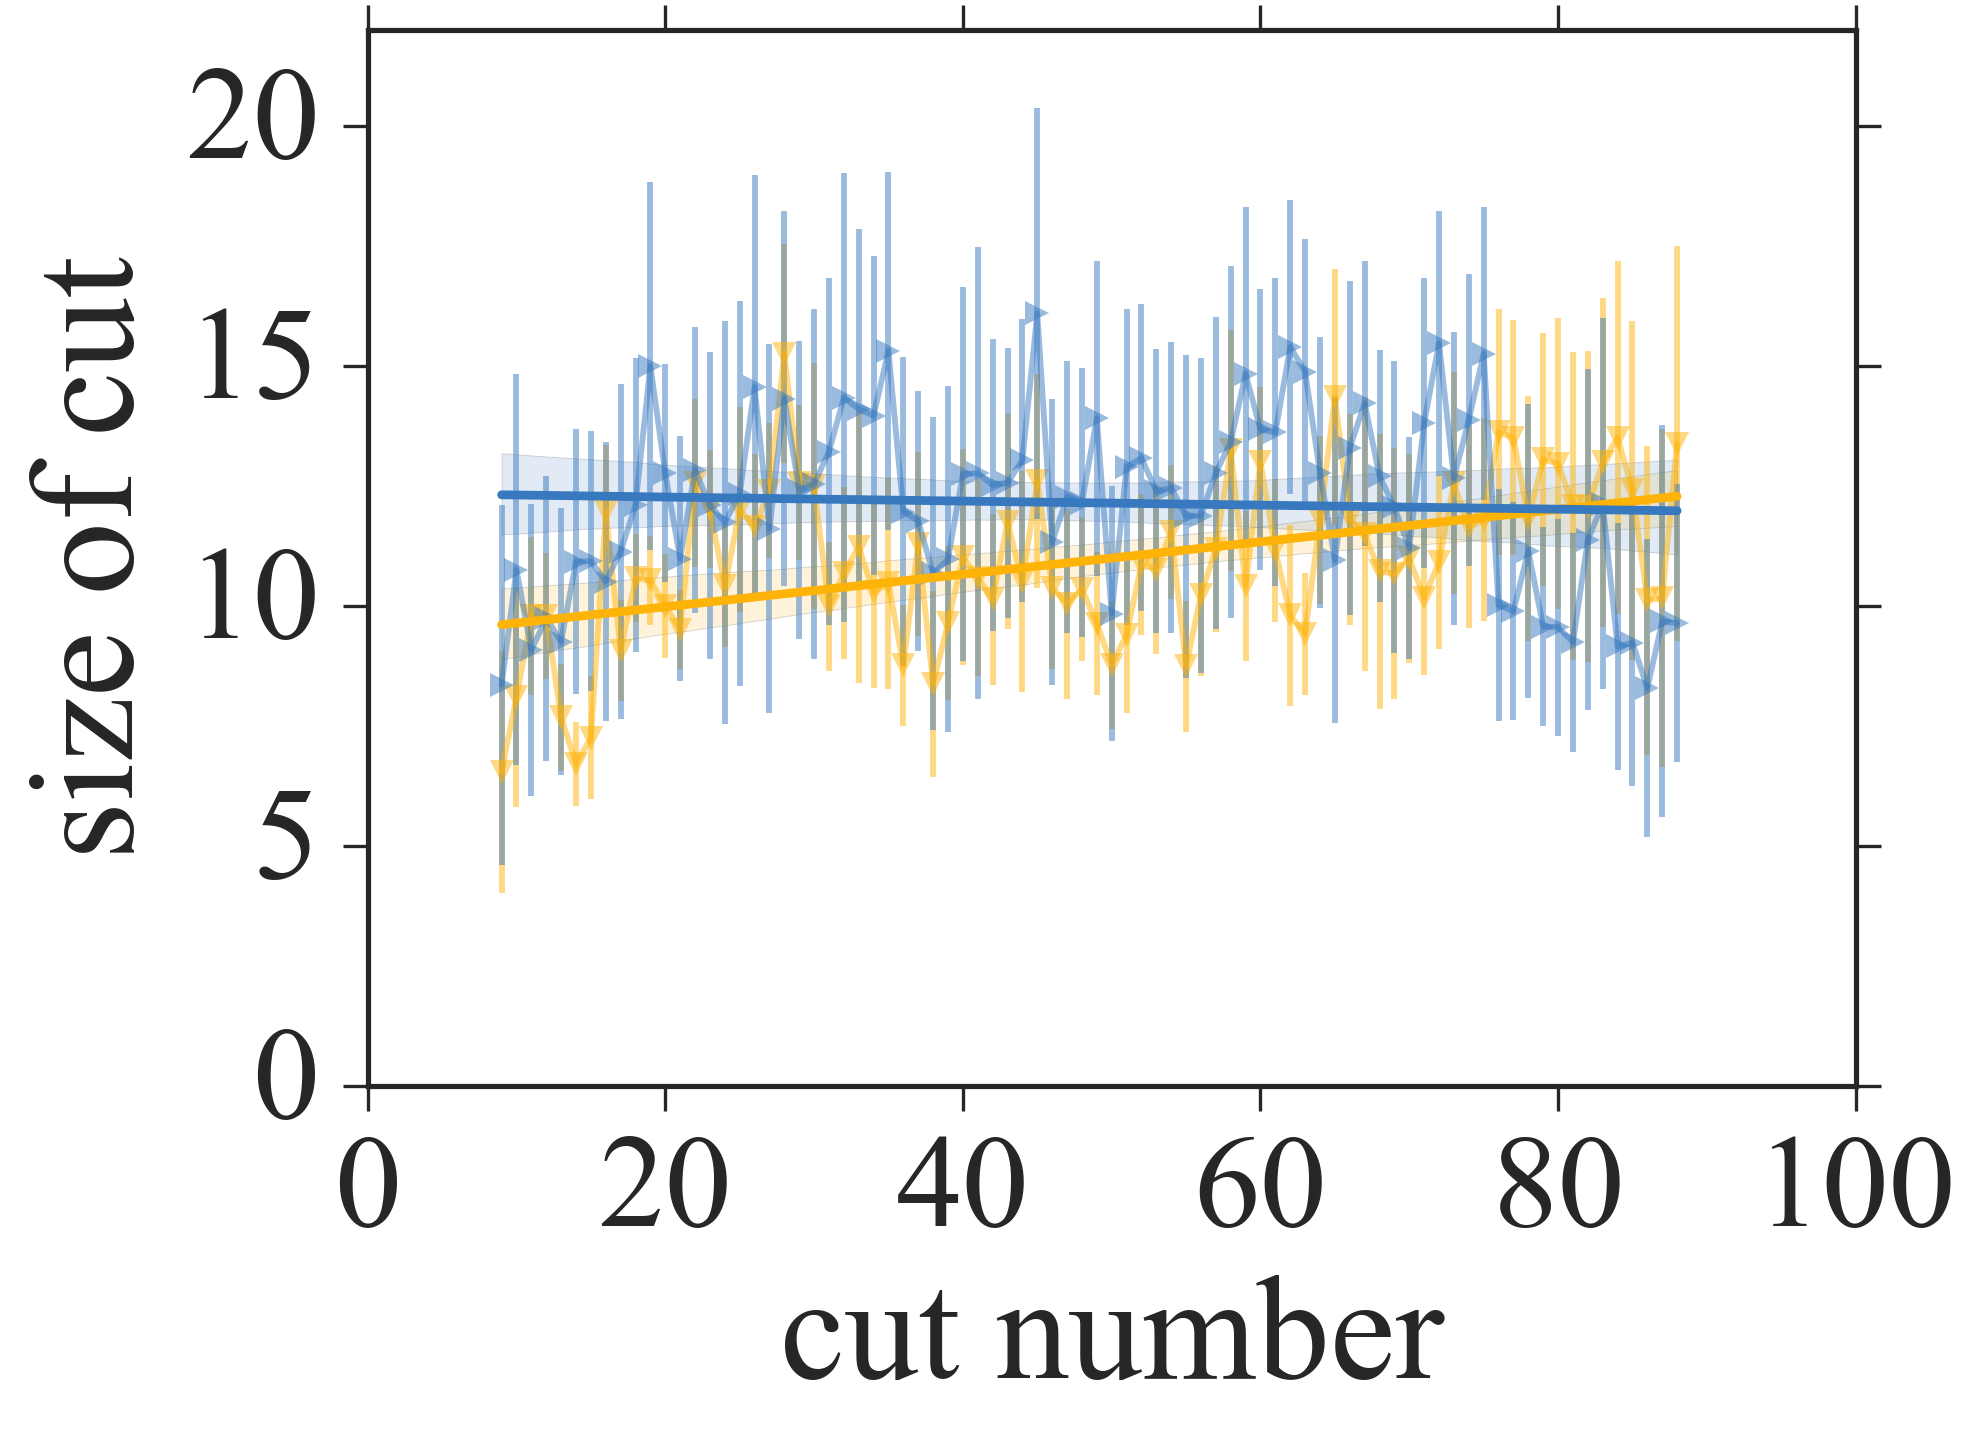
\includegraphics[width=\twoimageswide,keepaspectratio]{cuts/size_cuts_motion45.png}\label{fig:size_cuts_right}}
			\newline
			\subfloat[][]{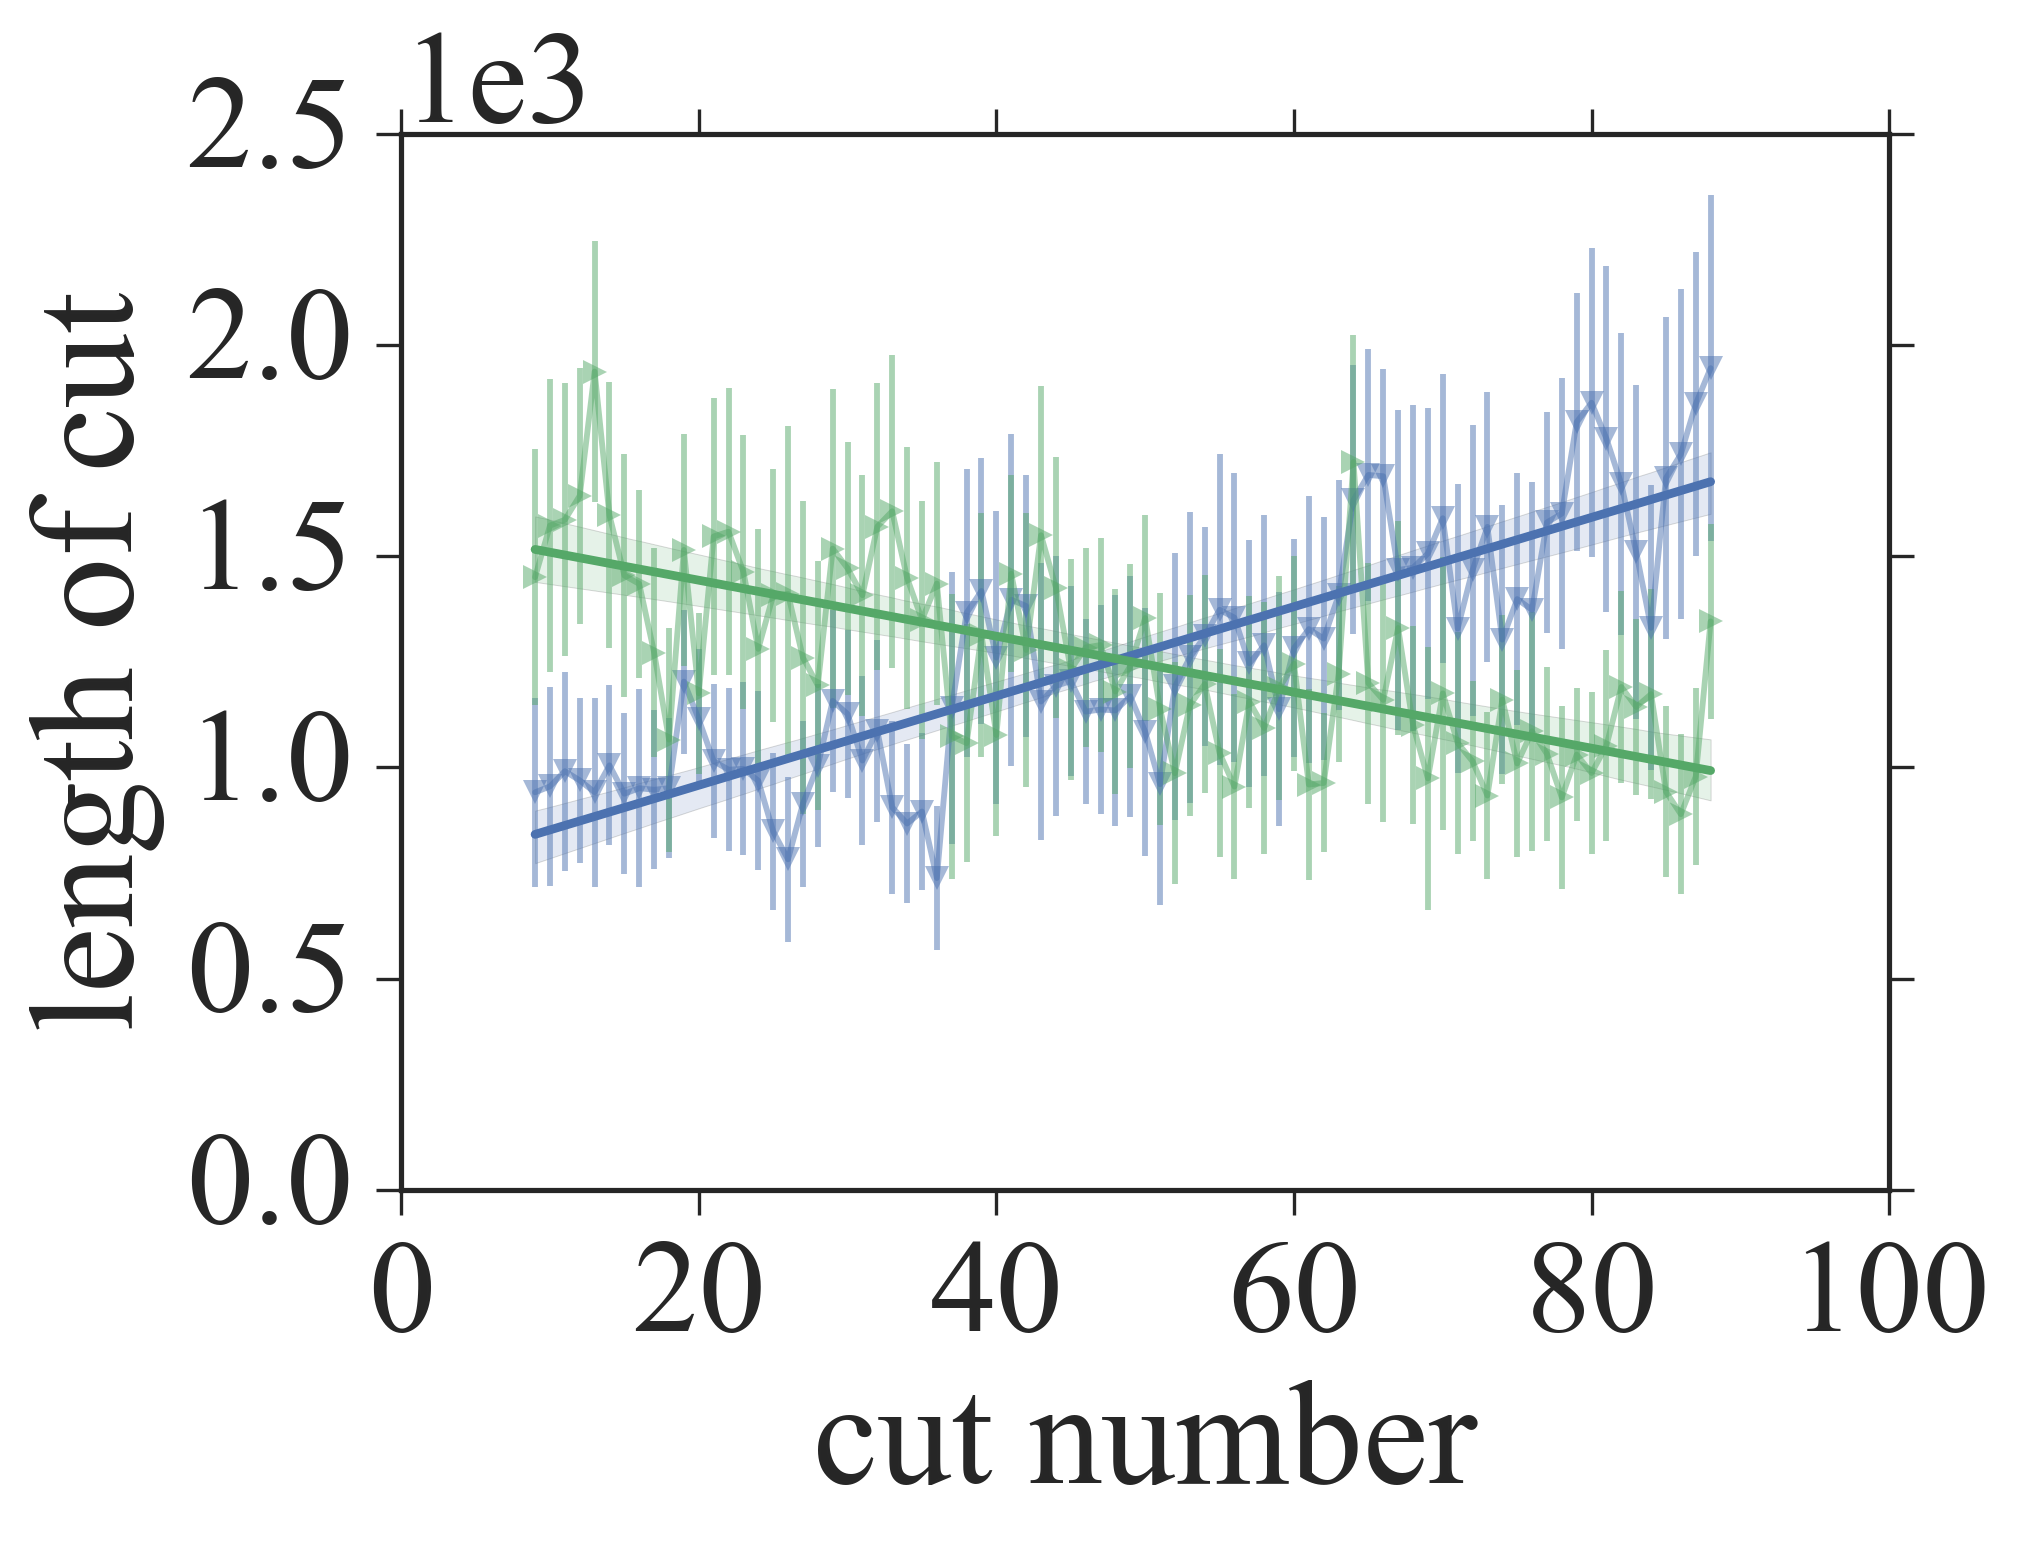
\includegraphics[width=\twoimageswide,keepaspectratio]{cuts/length_cuts_motion35.png}\label{fig:length_cuts_left}}\qquad
			\subfloat[][]{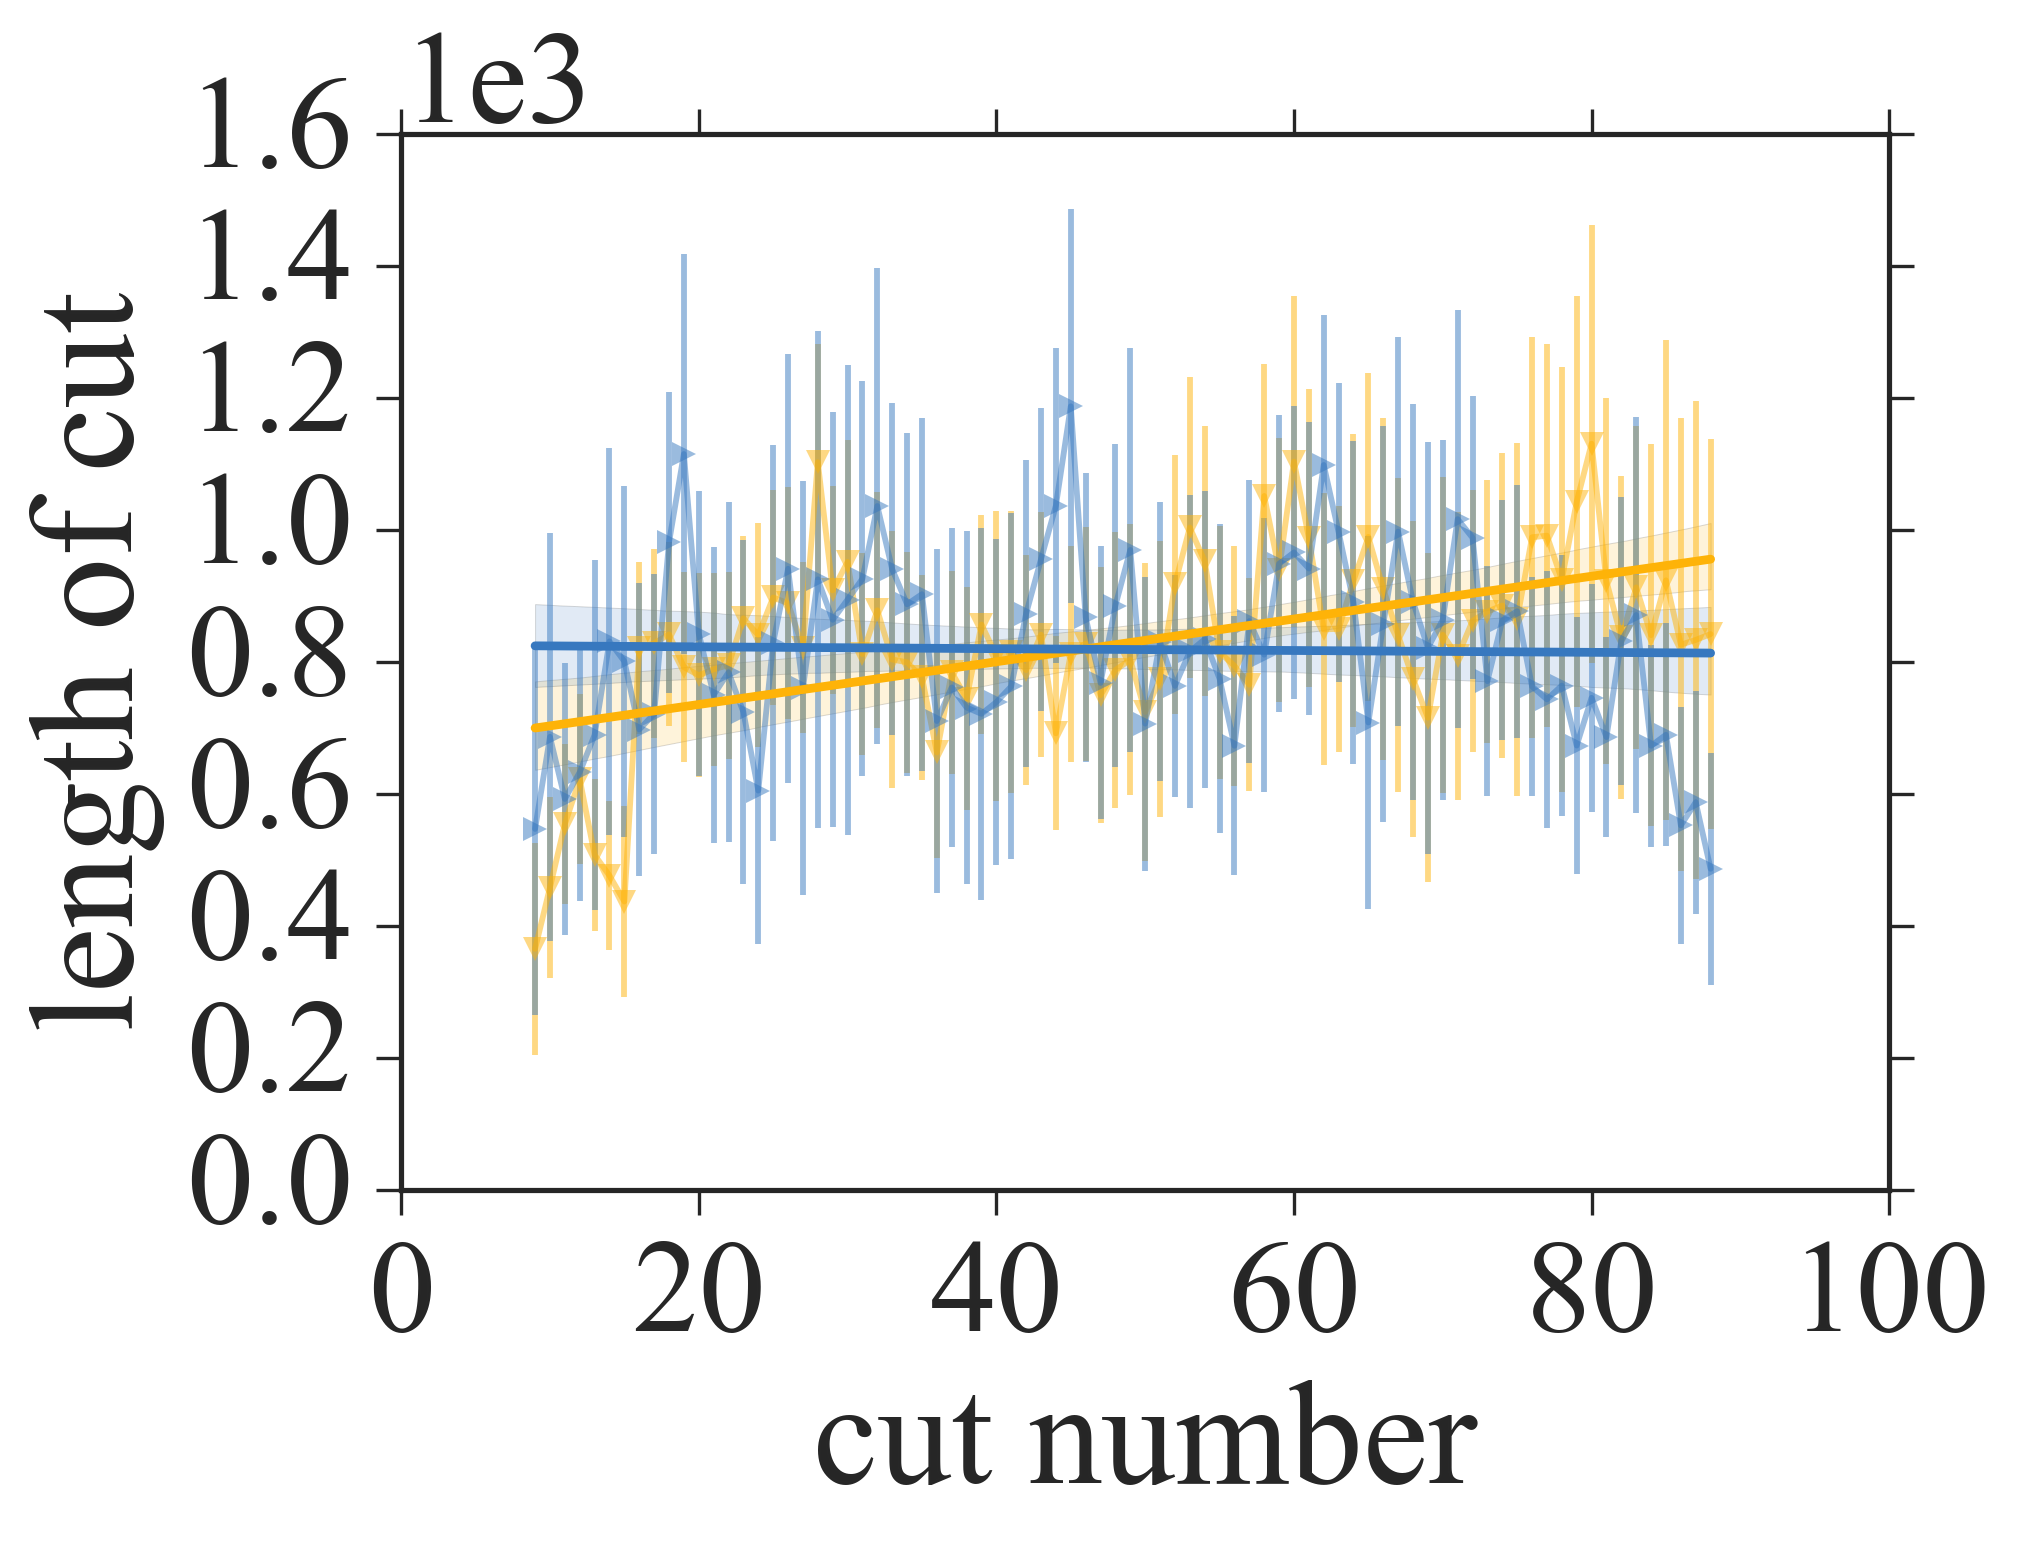
\includegraphics[width=\twoimageswide,keepaspectratio]{cuts/length_cuts_motion45.png}\label{fig:length_cuts_right}}
			\newline
			\subfloat[][]{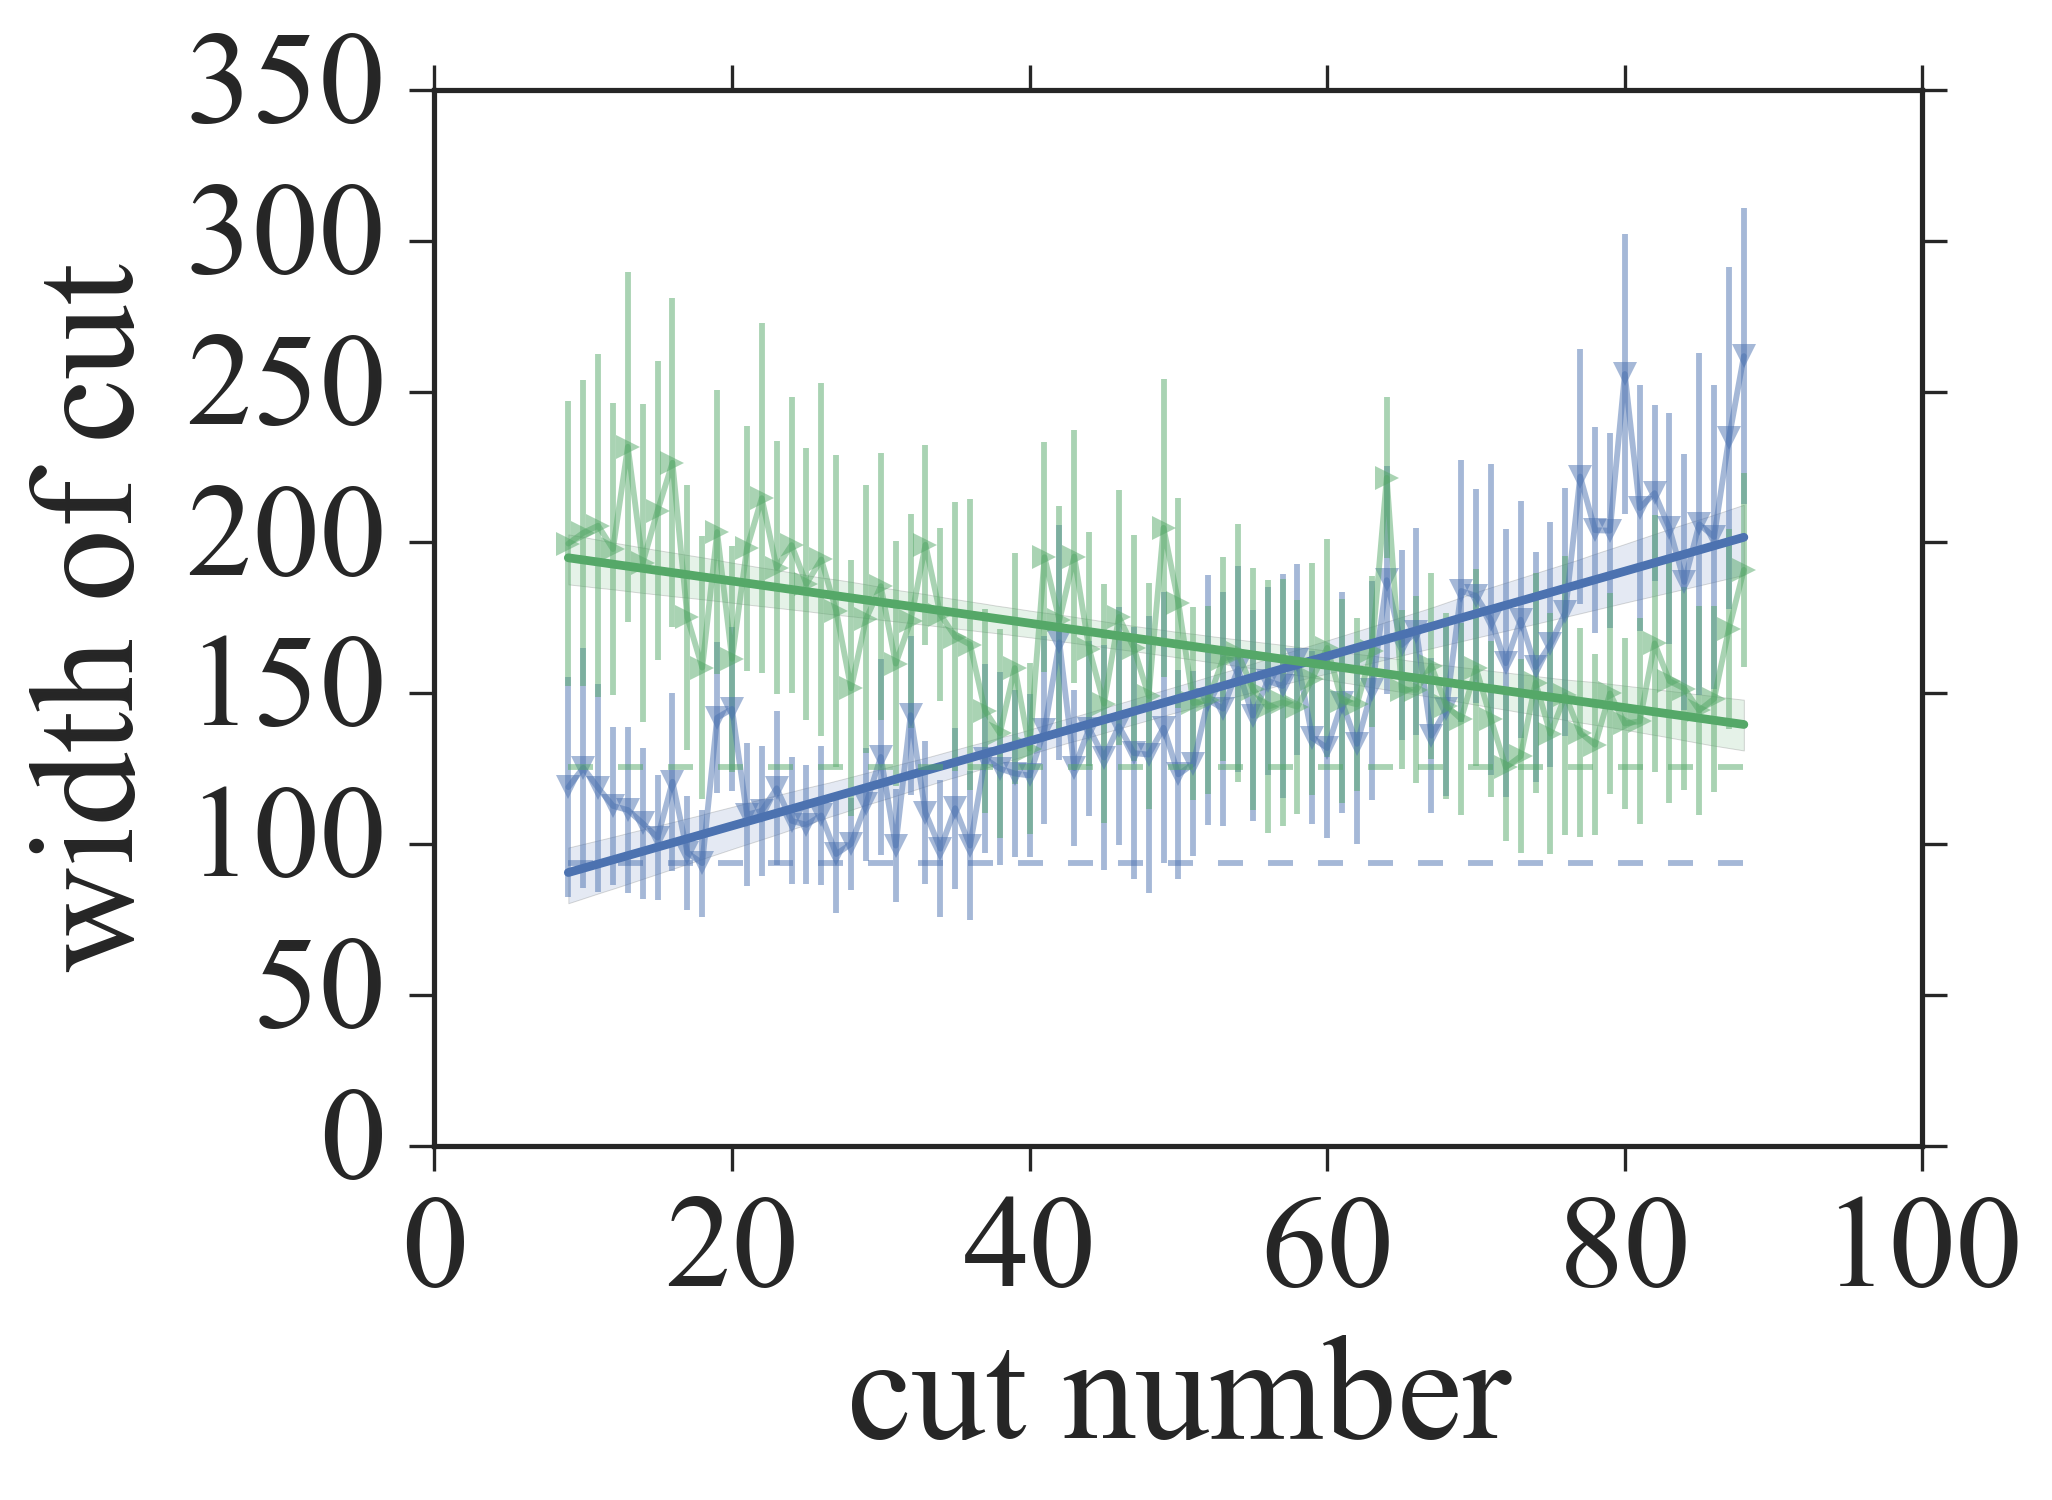
\includegraphics[width=\twoimageswide,keepaspectratio]{cuts/width_cuts_motion35.png}\label{fig:width_cuts_left}}\qquad
			\subfloat[][]{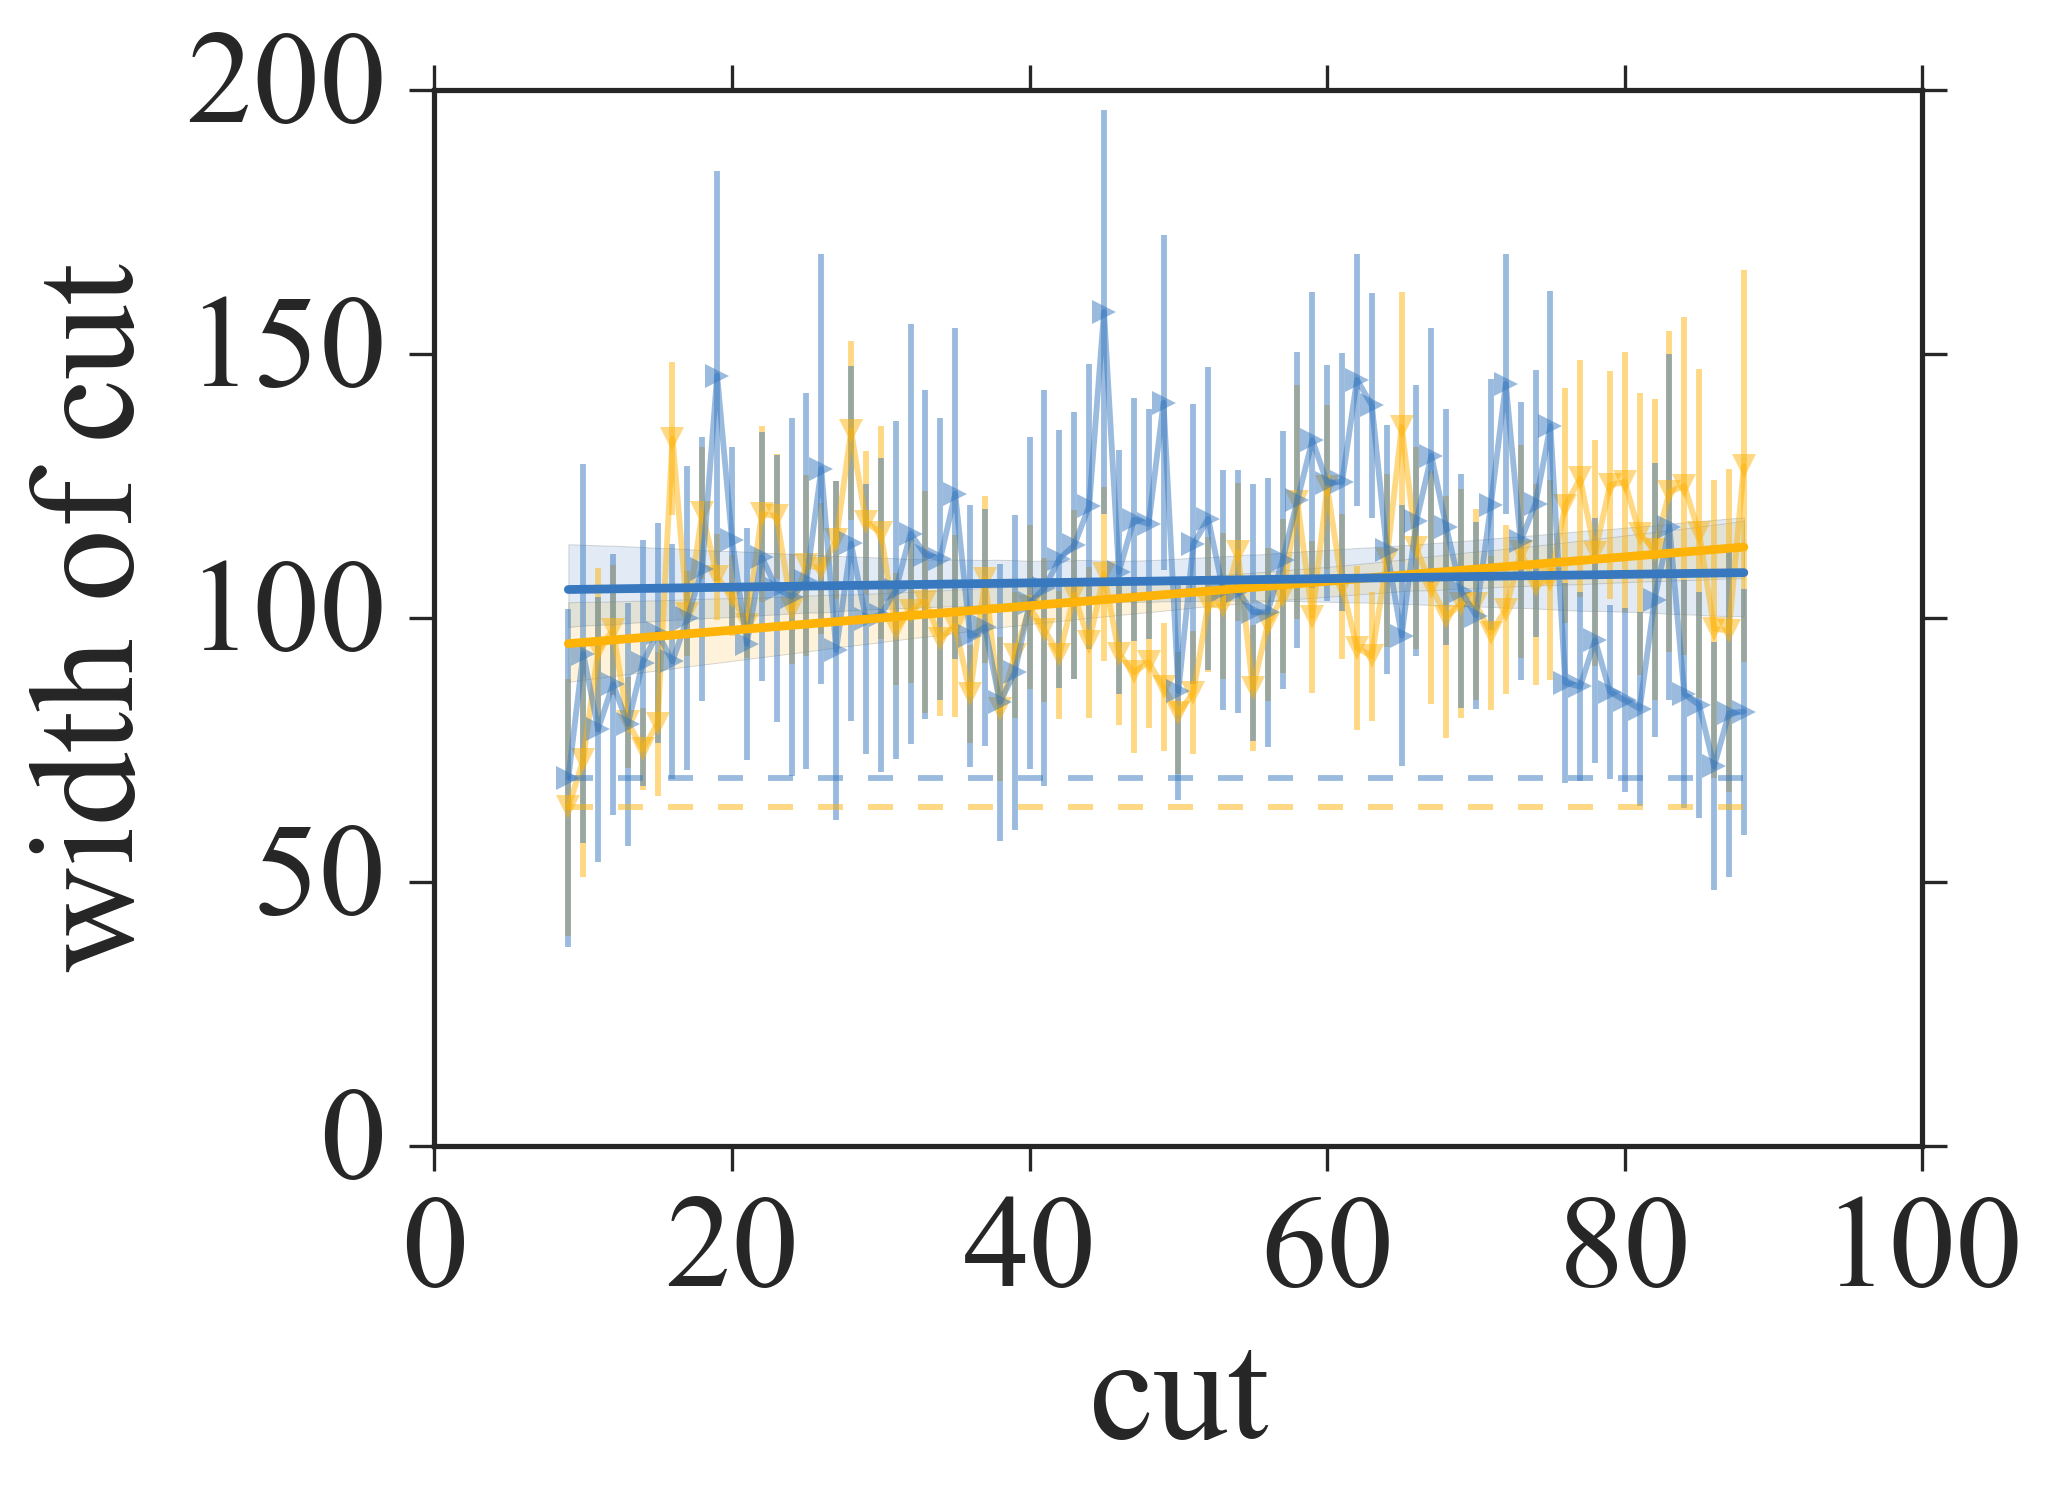
\includegraphics[width=\twoimageswide,keepaspectratio]{cuts/width_cuts_motion45.png}\label{fig:width_cuts_right}}
			
			\caption[Cut properties]{Cumulative cut properties for \series{35} (l.h.s.\ row) and \series{45} (r.h.s.\ row). The errors denote one sigma standard deviations. Solid lines give linear fits to the data intended to guide the eye. Green triangles pointing downwards belong to horizontal cuts (moving from top to bottom) while blue triangles pointing to the right illustrate vertical cuts (moving from left to right). Dashed lines illustrate the values of minimum width cuts.}
			\label{fig:cuts}
		\end{figure}

		The fact that some series exhibit distinctly different trends between horizontal and vertical cuts is curious. Why are the cuts in growth direction more stable than the cuts perpendicular to it? For an attempt to explain this, we take a closer look at the cut widths and their significance with regards to fluid transport. Assume that for the organism to advance its growing front, it needs to actively direct its flow towards the general direction it wants to expand towards. Given the experimental setup underlying the data we explore, this means the organism is advancing along the positive x-axis with an apical zone approximately parallel to the y-axis, see \Fref{fig:sup::physarum_expanding}. Thus any fluid flow proceeding along the x-axis must pass trough a sequence of vertical cuts. By virtue of the min-cut max-flow theorem, it is known that the maximum amount of flow that may pass through such a sequence is equal by the value of the minimum capacity cut. Intuitively, any attempt to push flow through a sequence of cuts is always capped by the amount of flow the bottleneck cut admits, see dashed lines in \Fref{fig:width_cuts_left} and \Fref{fig:width_cuts_right}. In light of this fact it seems natural for the sequence of vertical cuts to be balanced in width because this configuration allows for efficient fluid transport. We stress that in order to increase the fluid transportation capabilities across a sequence of cuts, only improvements of the minimum cut are effective. Increasing the capacity of any other cut implies higher material costs without any immediate benefits in terms of directed fluid transport. Thus balanced cuts provide the optimal ratio of material cost to transport capacity.

		While vertical cuts are well-balanced for almost all series, it is interesting to note that a significant number of series show unbalanced horizontal cuts. We find such cuts across all our data groups, which leads us to speculate that a significant structural difference between the two major directions of fluid transport is present. The fact that \P favors balancing vertical cuts over balancing horizontal cuts when expanding along the positive x-axis indicates that exploring new territory, \ie foraging, takes precedence over improving circulation within the existing network.

		Note, that our reduction of the complex flow patterns observed in \P to two cardinal directions is rather crude. However, our results yield a first quantitative indication that the growth direction is indeed intimately connected with distinct structural properties. It is worthwhile to think about more sophisticated methods trying to establish links between network growth and network structure in the future.

	\subsection{Percolation}

		Previously, concepts from percolation and graph theory where successfully combined to study the assembly of macroscopic \P networks from microscopic slime mold fragments, called microplasmodia~\cite{fessel2012physarum,fessel2014analytical,fessel2015structuring}. Here we shall take the reverse approach to add another item to the collection of characteristic \P properties. To do so, we start with a well-formed \P network and gradually disassemble or ``damage'' it until it becomes maximally fragmented. A network $G$ is damaged by removing nodes or edges successively in a random order. Removal continues until the graph is empty. The result is a sequence of graphs $\mathcal{S} = {G, G_1, \ldots, G_k}$ with a strictly decreasing number of edges or nodes. For each graph in the sequence one may then compute various observables and study their behavior with respect to the inflicted damage. This process has been successfully applied to various networks to determine the extend to which networks can remain operable despite of its components sustaining damage~\cite{callaway2000network,carlson2002complexity}. 

		Let us focus on random node and edge percolation. We define an occupation probability $p$ such that any given node $u$ or edge $e$ respectively is present in the graph with probability $p$. Equivalently, it is removed with probability $1-p$. For any graph $G_i \in \mathcal{S} $, we study the behavior of two important observables: the sizes of the largest and second largest connected components in $G_i$ as $p$ is varied from $0$ to $1$. We repeat this measurement $1000$ times for each graph in $\mathcal{S}$ and obtain averages and statistical errors for the measured quantities. 

		\Fref{fig:percolation_observables} shows the results for two graphs selected from \series{22} and \series{35} respectively. Let us first discuss the size of the largest connected component (LC). From the theory of percolation it is known that this quantity acts as an order parameter, signaling that as a certain critical occupation probability $p_c$ is reached, the system undergoes a (topological) phase transitions. For $p < p_c$ the size of the LC is very small, implying that the graph is fragmented, consisting of a large number of small connected components. Thus, it cannot function as a large connected unit. As we approach $p_c$ the situation changes abruptly and the largest connected component quickly grows to encompass the whole graph. Starting at $p=p_c$ the largest connected component is said to percolate, indicating that the graph may functions as one connected unit. Thus, if one removes less than a $1-p_c$ fraction of nodes or edges from a \P network, it is guaranteed to contain a large connected component whose size is comparable to the system size. Hence, the value of $p_c$ can be used to quantify the degree of damage a \P network can sustain whilst being able to maintain communication between almost all of its nodes.  

		\begin{figure}
			\centering
			\subfloat[][]{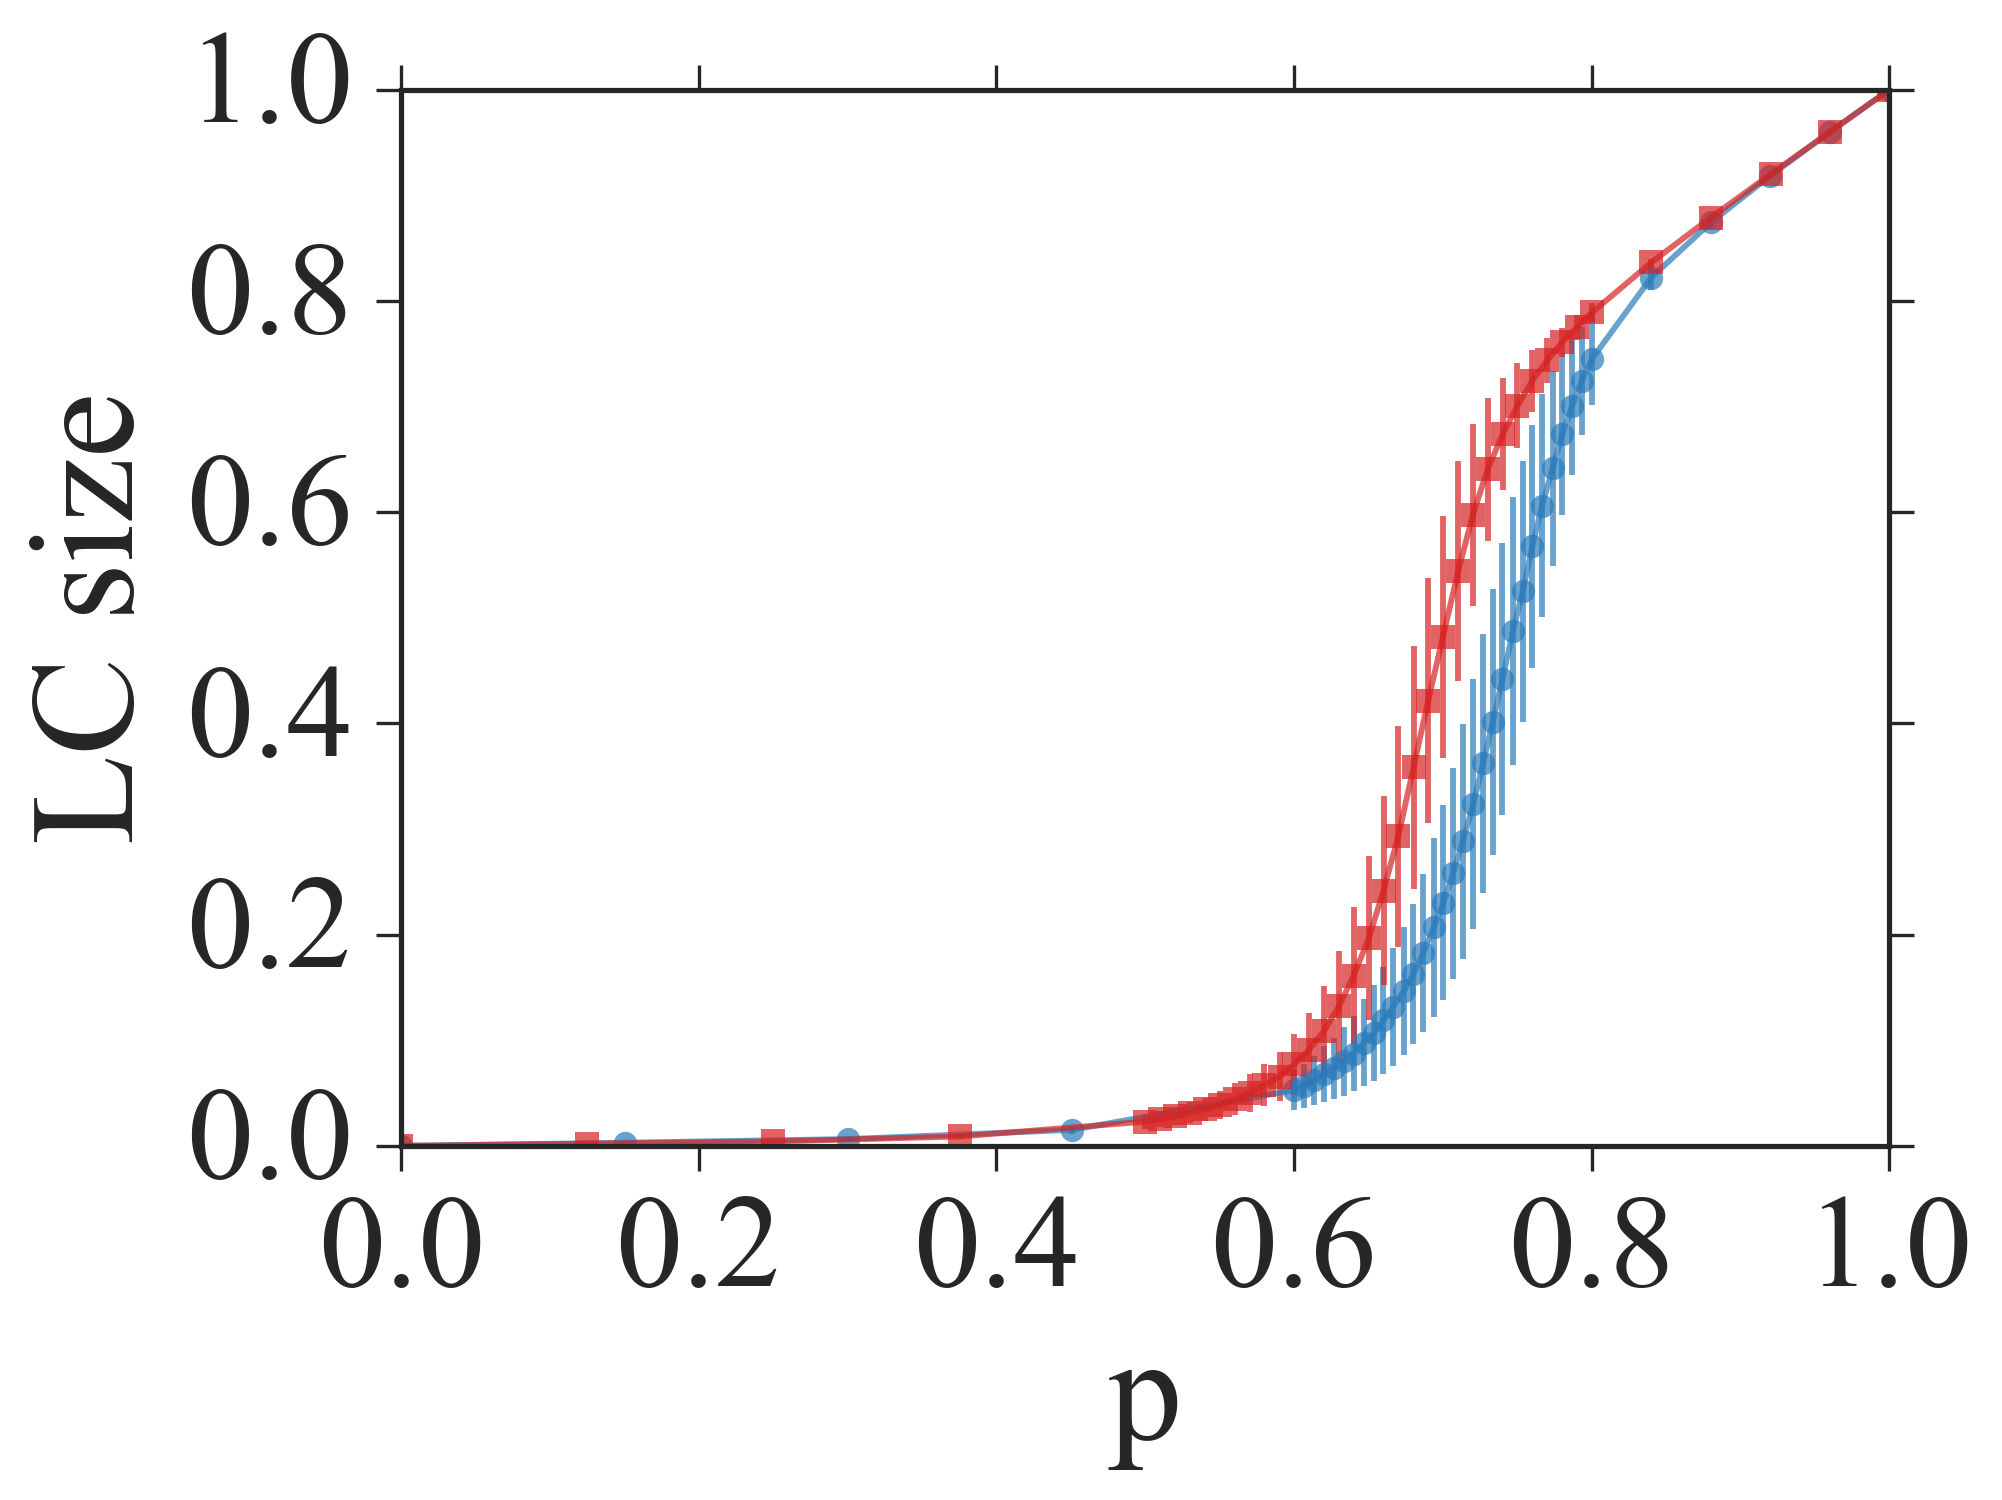
\includegraphics[width=\twoimageswide,keepaspectratio]{percolation/random_attack_largest_component_motion22.png}}\qquad
			\subfloat[][]{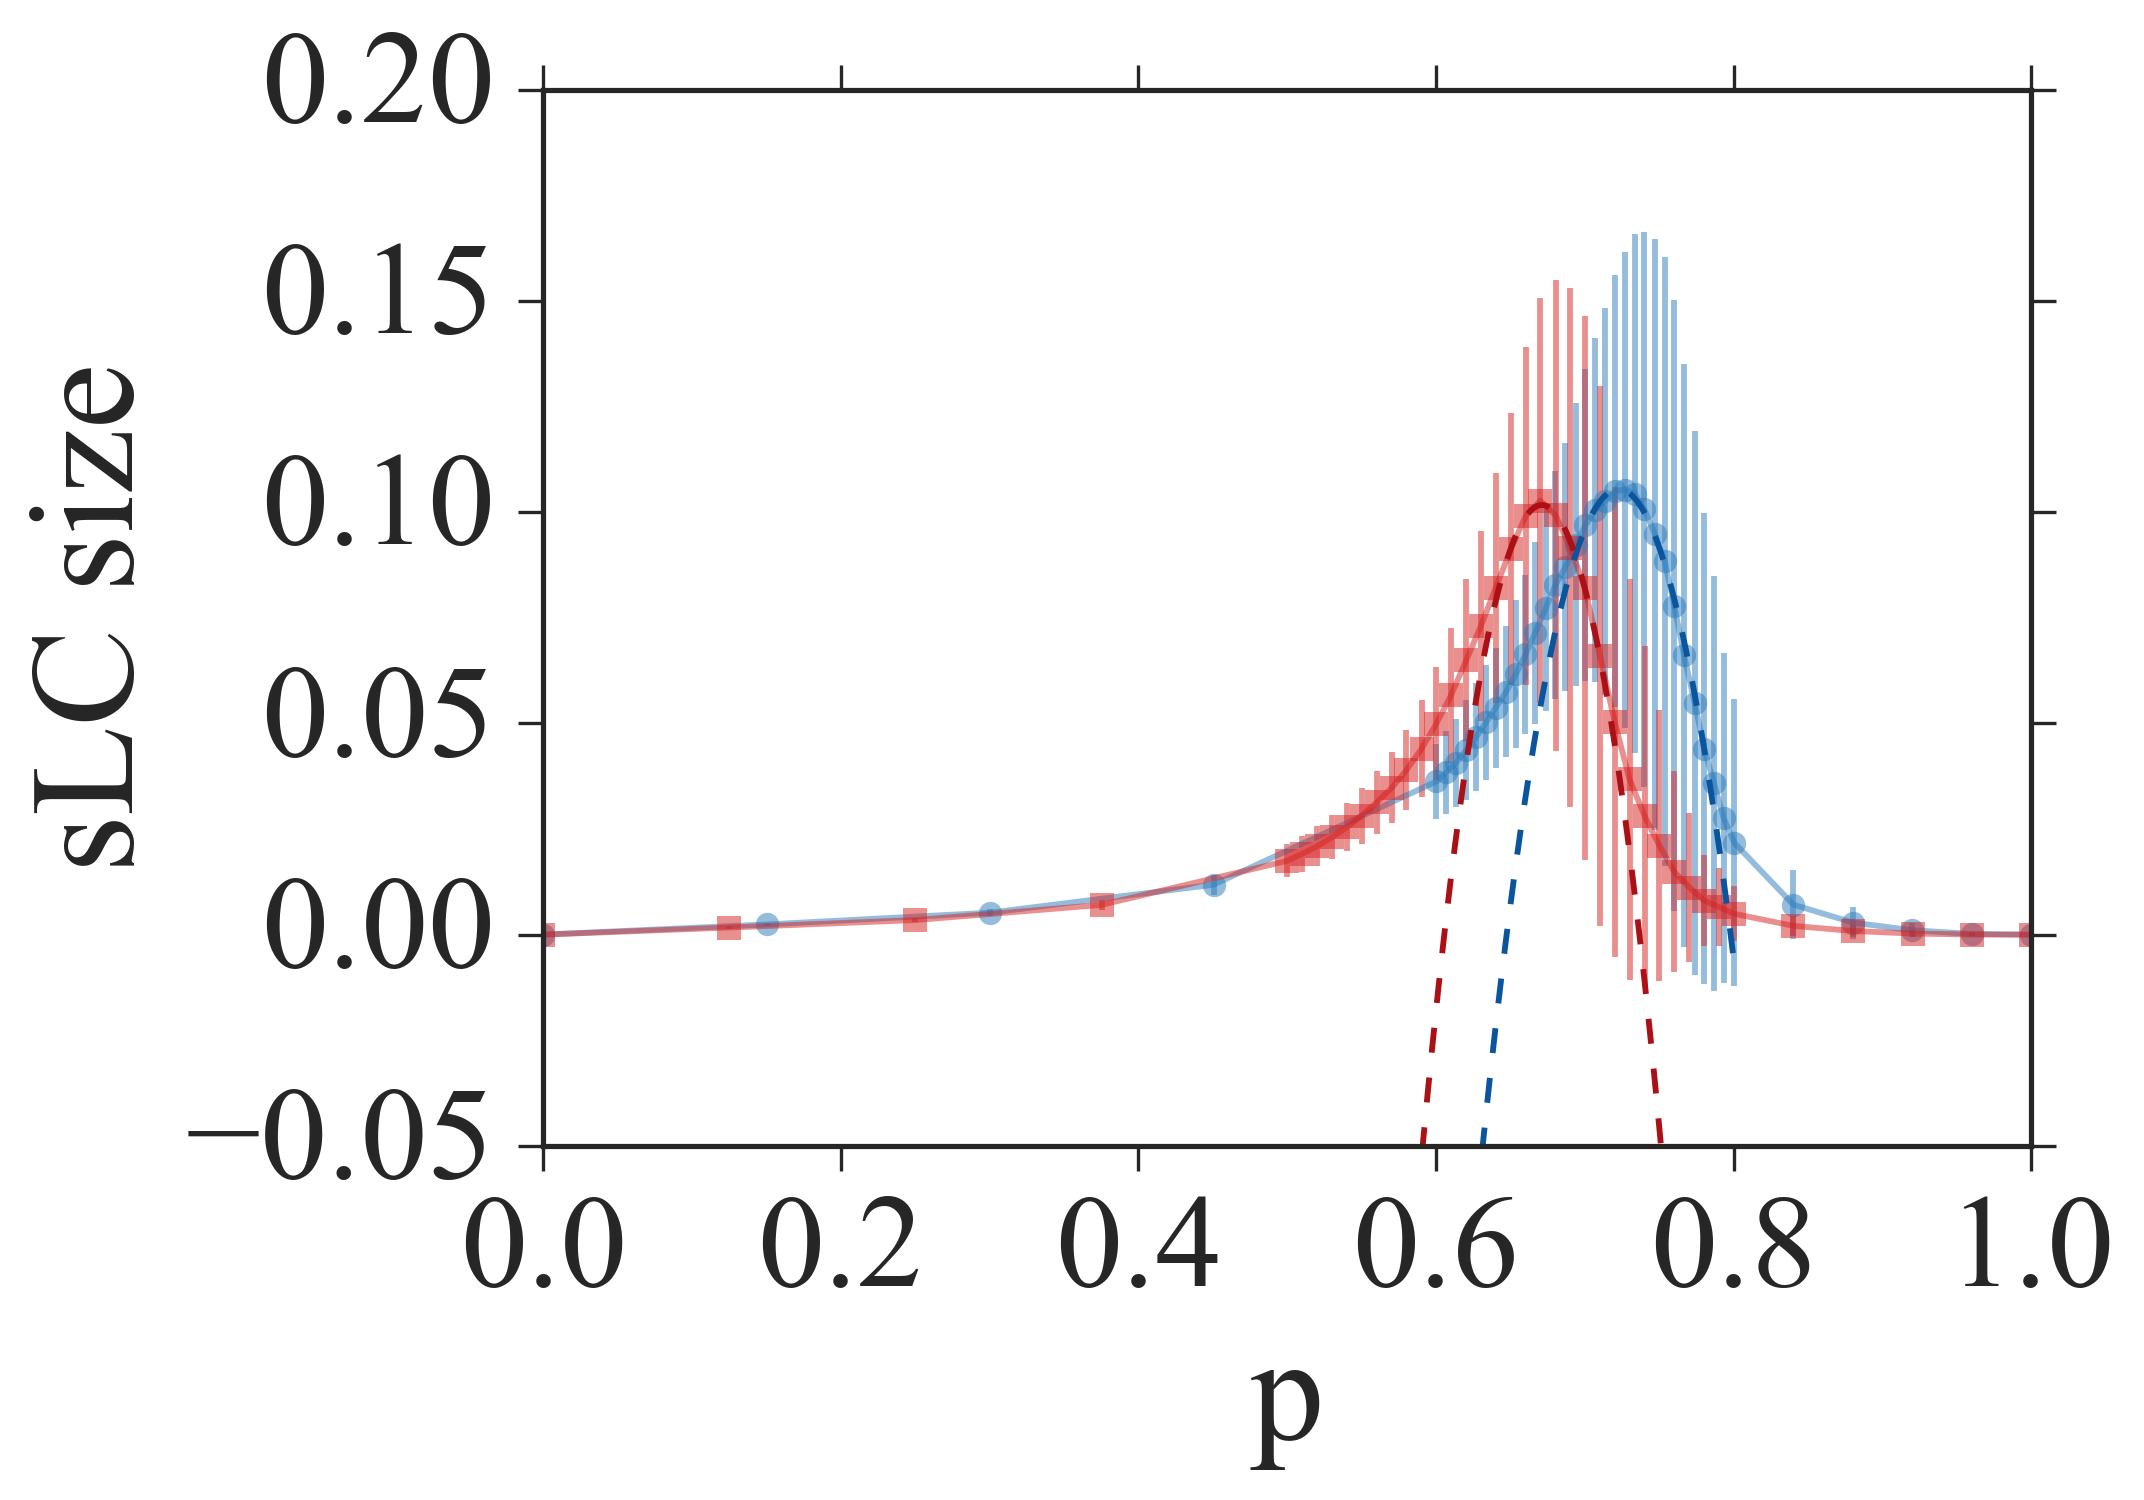
\includegraphics[width=\twoimageswide,keepaspectratio]{percolation/random_attack_second_largest_component_fit_motion22.png}}
			\newline
			\subfloat[][]{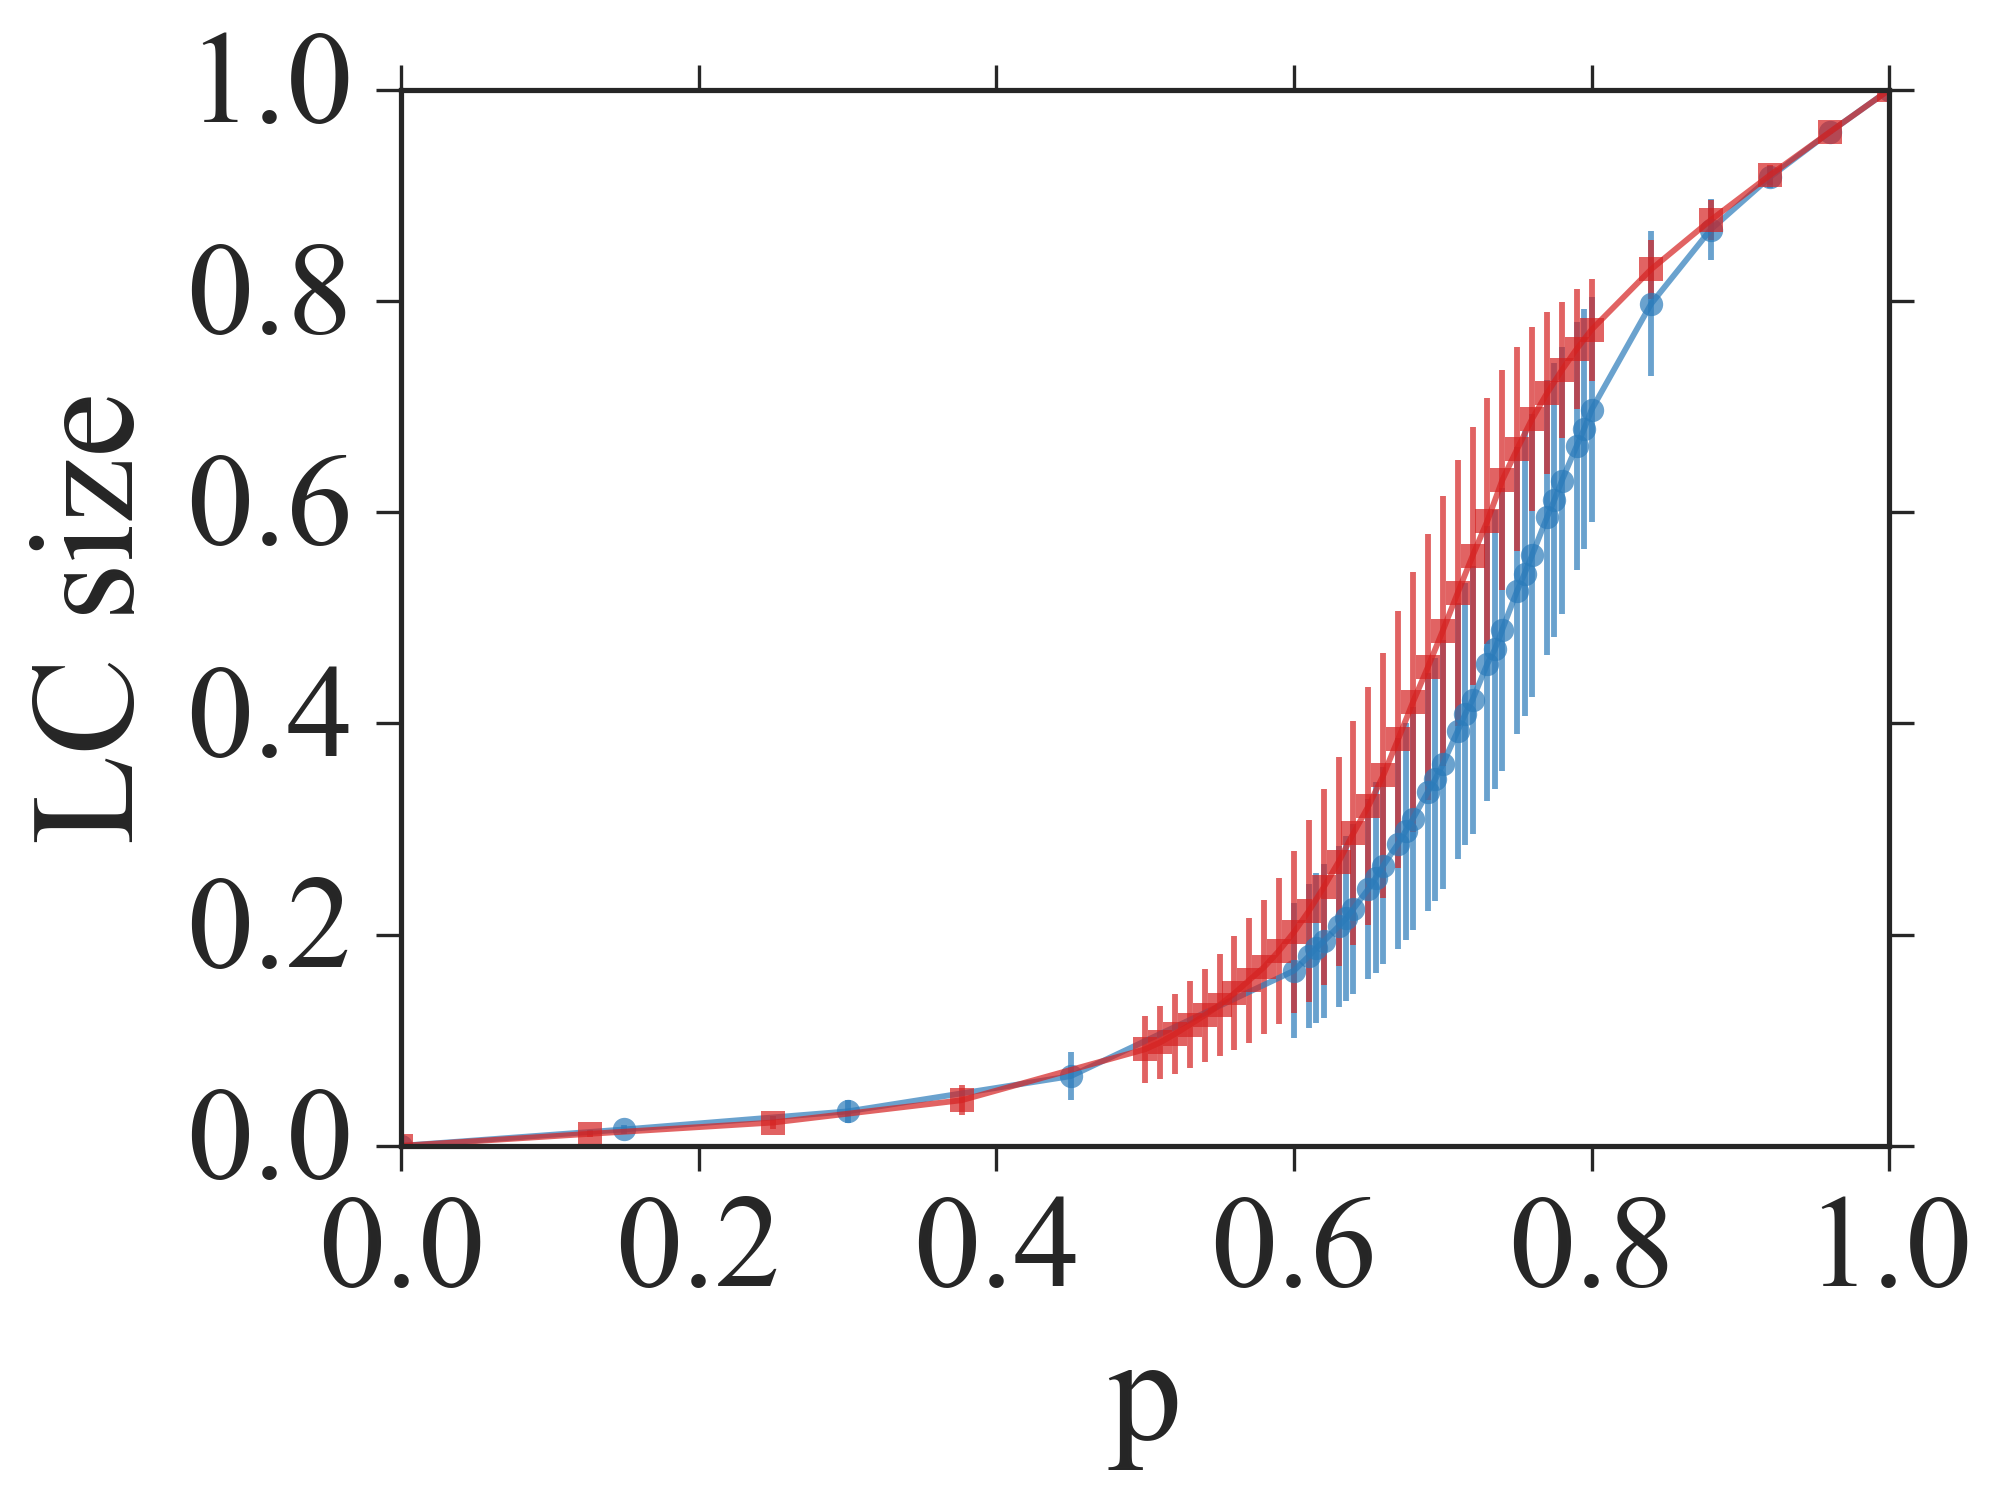
\includegraphics[width=\twoimageswide,keepaspectratio]{percolation/random_attack_largest_component_motion35.png}}\qquad
			\subfloat[][]{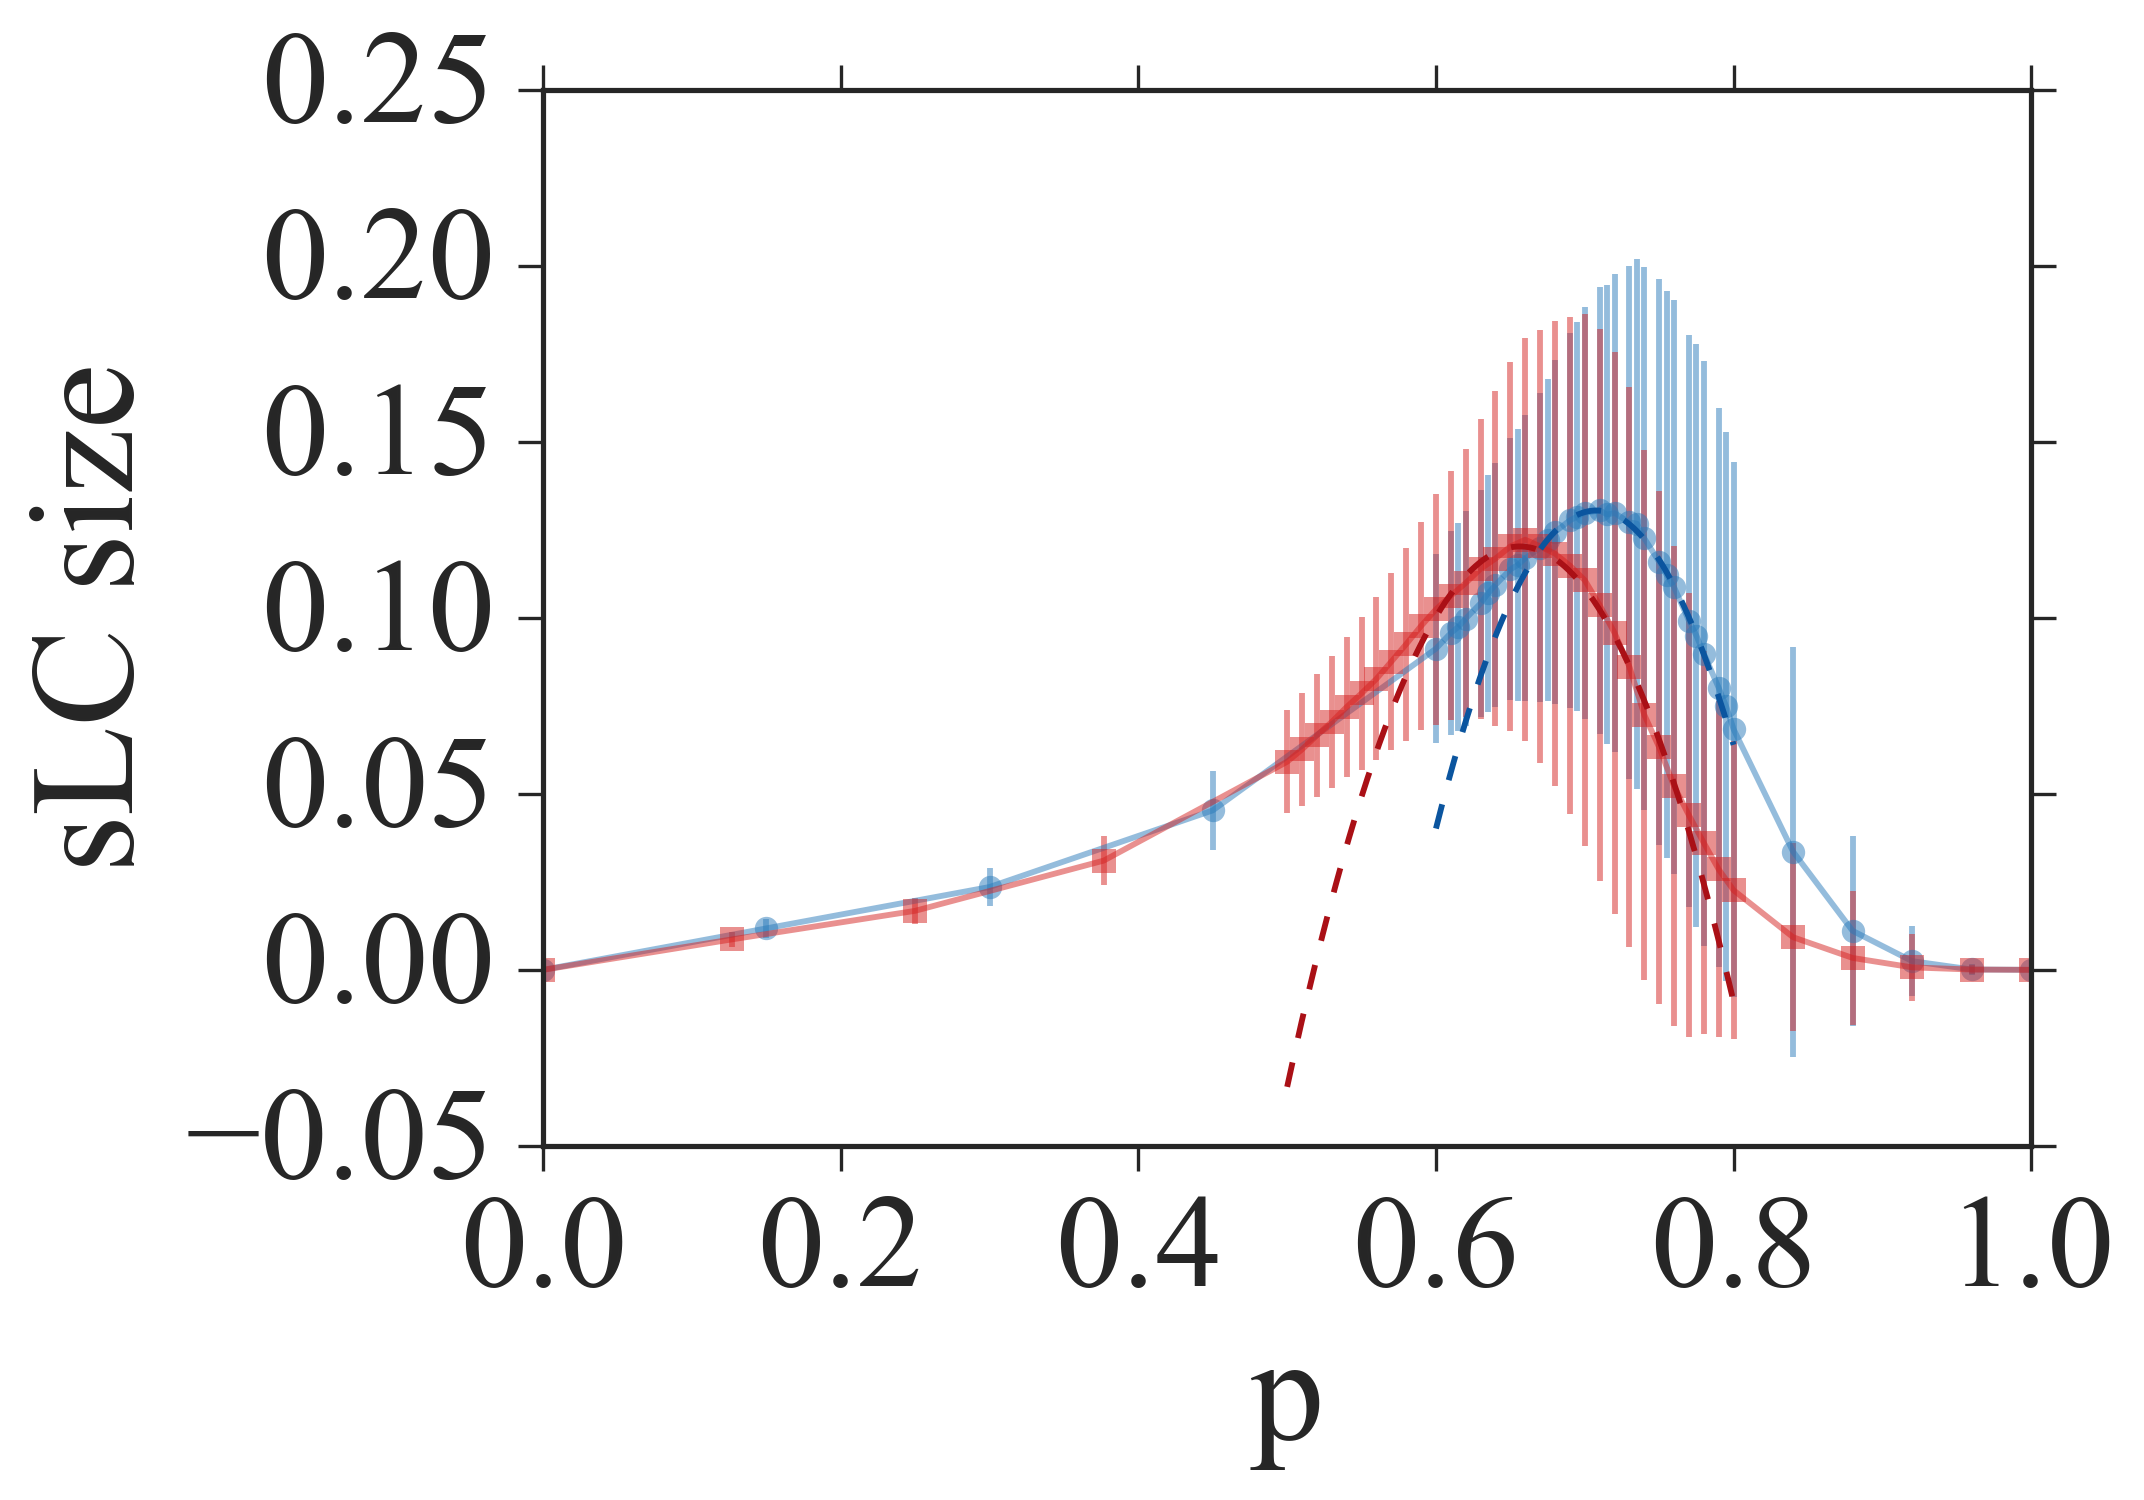
\includegraphics[width=\twoimageswide,keepaspectratio]{percolation/random_attack_second_largest_component_fit_motion35.png}}

			
			\caption[Percolation properties]{Percolation properties for a sample graph from \series{22} (top row) and from \series{35} (bottom row). The abscissa gives the occupation probability $p$. The ordinate shows the normalized size of the largest connected component (LC, l.h.s.\ column) or the normalized size of the second largest connected component (sLC, r.h.s.\ column). Red squares denote random node percolation, blue circles random edge percolation. For the second largest component sizes, parabolic fits approximate the location of the peaks as illustrated by dashed lines. Errors show one sigma standard deviations.}
			\label{fig:percolation_observables}
		\end{figure}

		
		To determine the value of $p_c$ we study the size of the second largest component (sLC). The theory of percolation predicts that this quantity diverges for $p=p_c$ on graphs of infinite size. On finite size graphs it becomes maximal. To obtain the location of the maximum, we fit the peak with a parabolic function

		\begin{equation}
			f(p) = a \ (p-d)^2 + c\,,
		\end{equation}
		where the value of the fit parameter $d$ approximates the value of the critical threshold $p_c$. It is also apparent that the critical threshold for random node percolation is larger than the one for random edge percolation. This is a general property of percolation and serves as a sanity check, suggesting that our simulations were performed correctly. It also dictates that \P graphs are more resilient to the removal of edges than to the removal of nodes.

		It is known that the critical threshold $p_c$ depends on the topology of the graph, the dimension of the space and the type of percolation, \eg node or edge percolation. \Fref{fig:percolation_observables} clearly shows that for a sample graph from \series{22}, containing some of our largest graphs, the size of the LCC increases faster around $p_c$ than for a graph from \series{35} containing much smaller graphs. At the same time the peak in the size of the sLC is less pronounced for the smaller graphs. These so-called finite size effects are expected and introduce a dependence on the graph size to $p_c$. As a result, what we are measuring for individual graphs is an effective finite size percolation threshold $p_c(L)$. Here $L$ denotes the number of nodes $n$ in case of node percolation and the number of edges $m$ in case of edge percolation. Naturally, we are interested in the so-called thermodynamic limit, \ie $p_c(L)$ for $L \to \infty$. 

		To get an impression of the dependence of the system size $L$, \Fref{fig:percolation_scaling} shows the values of $p_c$ for the collective data. It can be seen that the critical values vary with the size of the system as expected. For small $L$ critical values are smaller than for larger $L$ where they seem to become constant. Extracting this constant value for $L \to \infty$ is the objective of finite size analysis. In it, relying on the theory of critical phenomena, a scaling function is derived, which captures finite size corrections as a function of the system size $L$ and a small set of critical exponents. 
		
		\begin{figure}[!htbp]
			\centering
				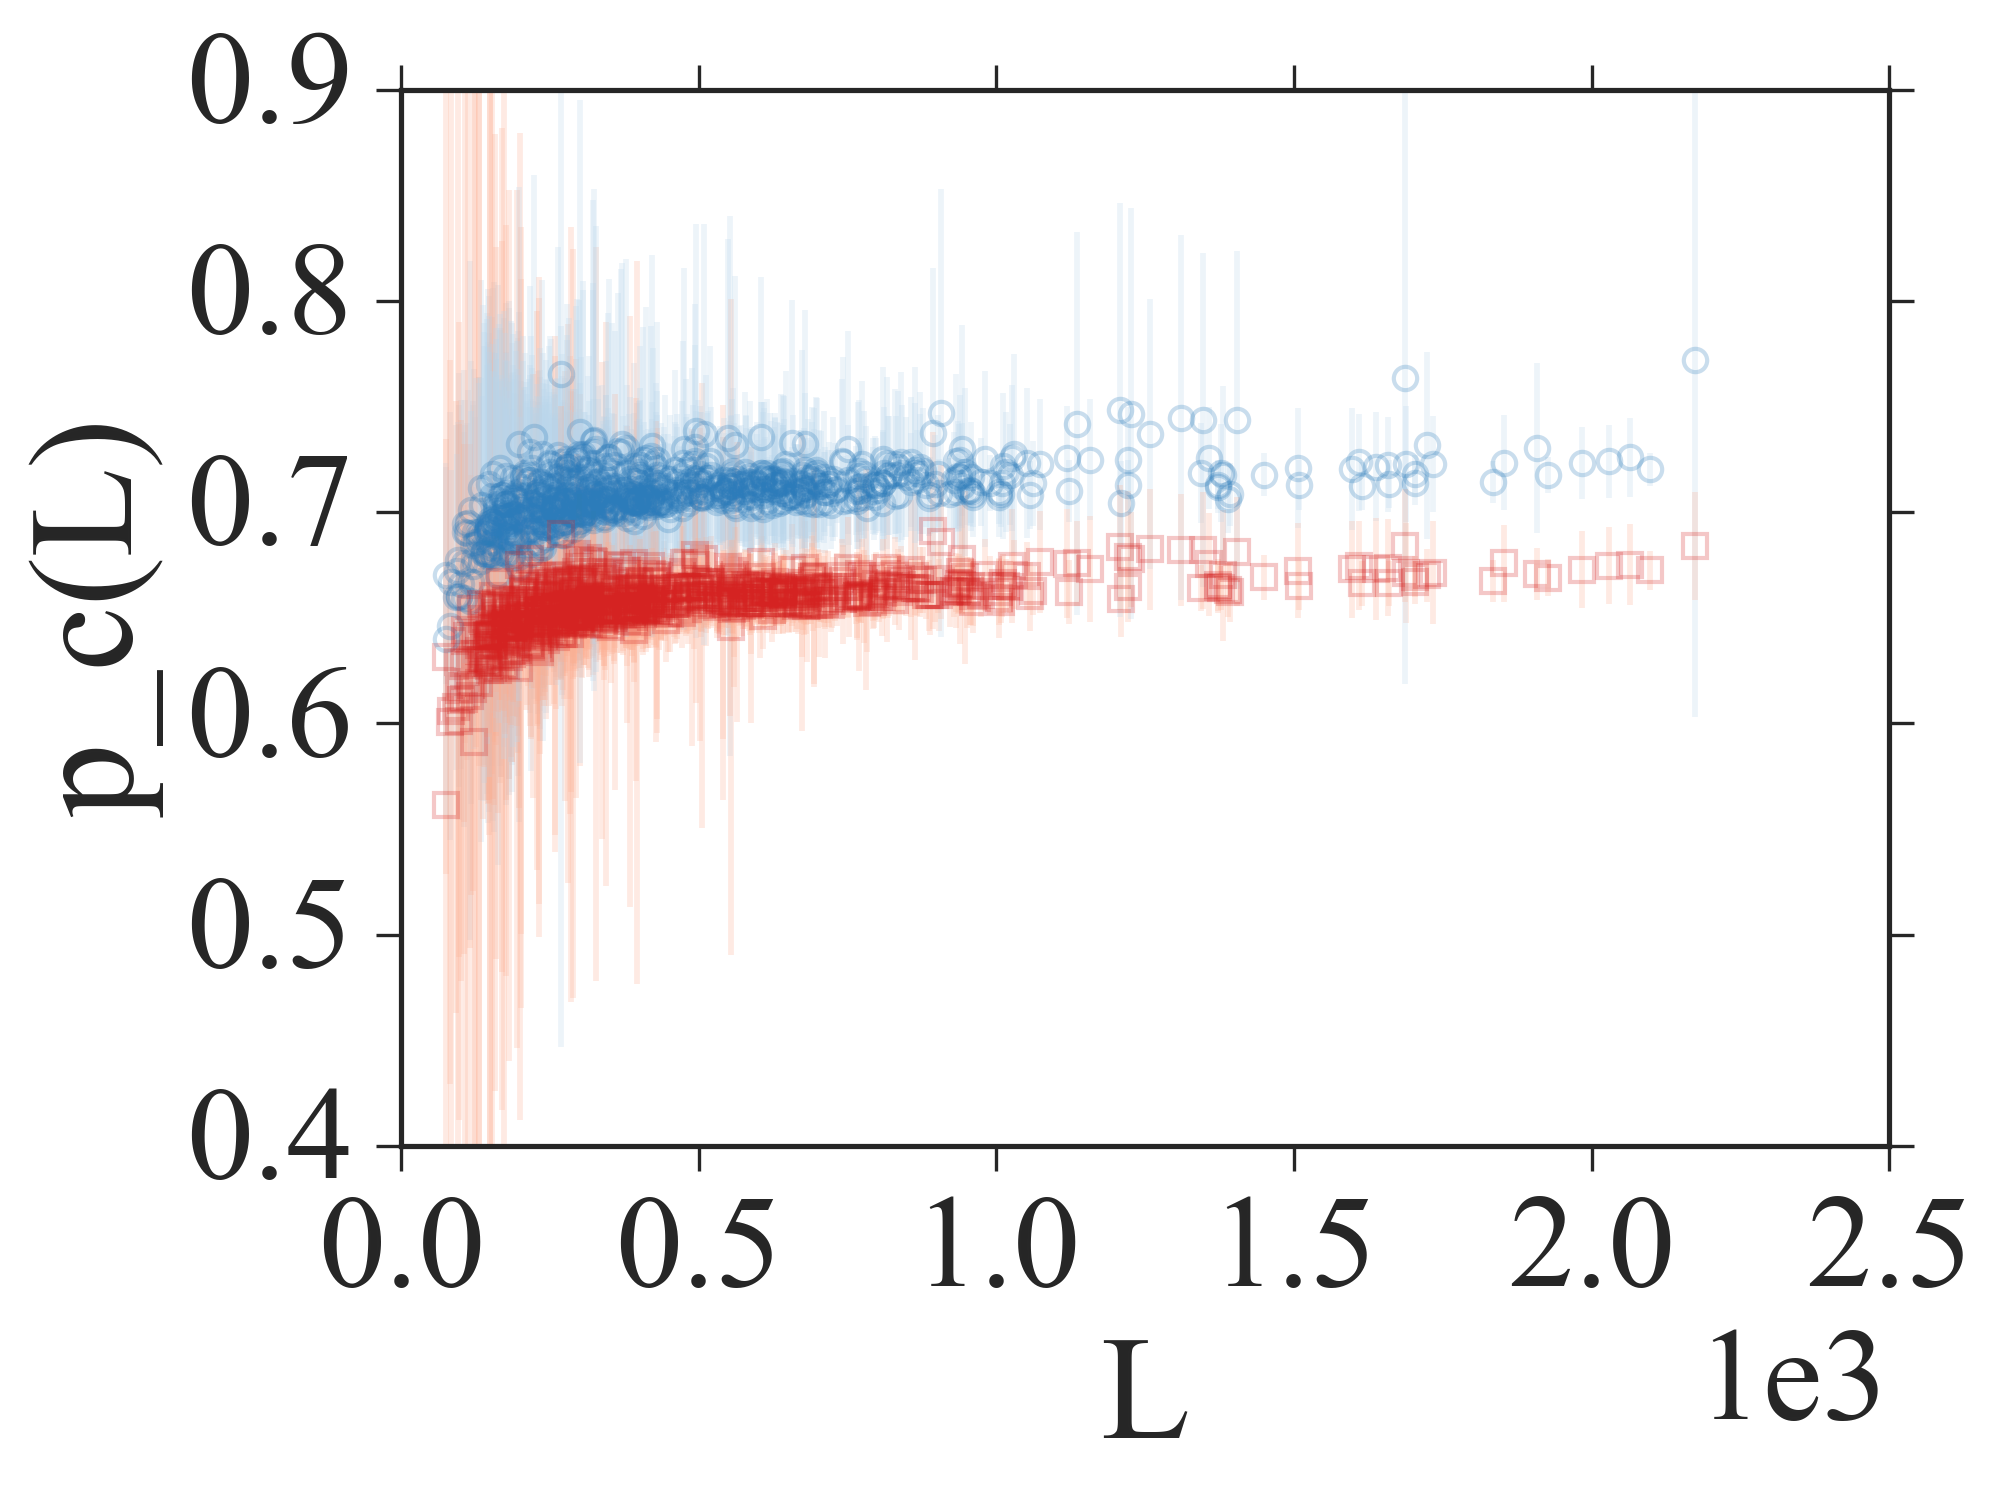
\includegraphics[width=0.55\textwidth]{percolation/random_attack_second_largest_component_fit_cummulative.png}
			\caption[Critical percolation thresholds]{Dependence of the critical threshold $p_c(L)$ for all available \P graphs on the size of the graph $L$. Blue circles refer to random node percolation, red squares to random edge percolation. Dashed lines indicate scaling fits.}
			\label{fig:percolation_scaling}
		\end{figure}

		As a possible scaling law we propose an \textit{Ansatz} of
		\begin{equation}
			p_c(L) = a + b L^{c} + d L^{e} + f log(L)^{g}\,,
		\end{equation}
		where we add a logarithmic term to the polynomial expression to allow for sub-leading corrections, without which scaling fits may fail, particularly on small size systems. Furthermore we restricted the exponents $c,e$ and $g$ to negative numbers to obtain a finite value of $p_c(L)$ as $L \to \infty$. The resulting fits are shown in \Fref{fig:percolation_scaling}. Note that for small $L$ the fit is lacking as it overestimates the values of $p_c(L)$.  Furthermore it appears that for large $L$ the available data points are underestimated. The effect is small but seems to be systematic. It likely causes us to underestimate the final critical thresholds in the thermodynamic limit. The thresholds are $p_c = 0.7118 \pm 0.0544$ for random node percolation and $p_c = 0.6584 \pm 0.0217$ for random edge percolation. Note that compared to other numerical percolation results, the error of both quantities is very large and thus the obtained values are to be taken as a rough approximation only.

		Let us discuss potential reasons for the large uncertainty in the critical values. First, the graphs we use might be too small. It is known that the reliability of percolation studies increases with larger system sizes. However, the values for $p_c(L)$ in \Fref{fig:percolation_scaling} appear to be relatively stable in the limit of large $L$. This does suggest that the graphs are large enough to observe finite size scaling properly. On the other hand, there is only a limited sample of larger graphs which this observation is based on. Also smaller graphs dominate our data in comparison to large graphs may lead to diminished accuracy of the fits. We have experimented with excluding the smaller graphs from the set, but imposing arbitrarily chosen size thresholds did not significantly improve the fits. A real improvement can probably only be achieved by increasing the number of large graphs that enter the analysis.

		Second, it is possible that our choice of a scaling law is suboptimal. After searching the literature, we only found one alternative option to our scaling choice in an earlier percolation study focusing on graphs that are topologically similar to \P networks. While the alternative looked promising on paper, it was not able to satisfactory fit our data. Thus we had to eliminate this option. An additional downside of the general scaling law we proposed is the resulting difficulty in interpreting the fit results in terms of meaningful critical exponents. Further studies are necessary to obtain reliable results in this regard.

		Third, it is conceivable that scaling fails because of a natural variability present in \P graphs. It is apparent from \Fref{fig:percolation_scaling} that points with similar $L$ can still differ considerably in $p_c(L)$. This is surprising because, if we assume that there is one complex physical process responsible for the observed topology of the graphs, one would expect it to produce networks that exhibit the same percolation properties for systems of identical size. Either this assumption is incorrect, or we must admit that other, possibly random, effects are responsible for the observed deviations. Candidates are minor variations in the experimental setup during culturing or other unknown environmental effects influencing the network formation of \P.

		Finally, let us compare the obtained approximate critical thresholds with those of two other structures which are planar, $3$-regular and well-studied in the context of percolation: The honeycomb lattice with $p_c = 0.6962(6)$ and $p_c = 1-2 sin (\pi/18) \approx 0.6527$ and the 2D Voronoi Tessellation\footnote{The point set for the tessellation is Poisson distributed in the plane.} with $p_c = 0.71410(2)$ and $p_c = 0.666931(5)$~\cite{djordjevic1982site,becker2009percolation}. Cited values denote node and edge percolation respectively. The similarity between the critical thresholds indicates that these structures exhibit a similar degree of resilience against random attacks. Where hexagonal lattices are clearly too regular to resemble \P, Voronoi graphs are more interesting. It is intriguing to see that the percolation of \P networks seems almost identical to percolation on Voronoi graphs. Are there similarities between the way \P grows in search of food and the way Voronoi graphs form? It is worthwhile to investigate these question in detail in the future.


	\section{Discussion}

		In this chapter we investigate $36$ time-series of \P graphs based on the \data available in the \SMGR. This amounts to a total of $1998$ graphs under consideration, which to the best of our knowledge, makes this study the largest of its kind available today. We present a investigation of this data leading to a comprehensive collection of various descriptive properties of \P networks. Let us first discuss the results individually and then comment on their combined usefulness.

		Paths can be regarded as the atomic building blocks of \P networks since they correspond to veins carrying protoplasm. We find that our data does not allow to unambiguously determine the underlying theoretical distribution of path lengths and average path widths, however, fitting gamma distributions slightly outperforms other distribution choices. Relying on gamma fits, we explore the time development of the distributions and find behavior that is consistent with network coarsening for a large number of data series. We determine a range of parameters that captures the distributions of path lengths and average path widths one may expect to observe in \P networks. In particular we find a linear relation between fit parameters for the average path width. Within the range of observed values, this means that the variation in the path width distribution is small, \ie the mode of the distribution is confined to a small interval. This is not the case for path lengths, which may display larger variations. With regards to network coarsening, it follows that the tendency to replace short veins with long ones is more pronounced than the tendency to replace thin veins with thick ones.

		In order to obtain more information about the structure of \P networks we introduce the study of its faces which correspond to cycles formed by veins.	Here we determine the distribution of physical aspects of faces such as the number of paths in a face (face degree) as well as its area and circumference. Unfortunately, we are not able to determine the underlying distribution with certainty, but find that gamma distributions capture face degree, area and circumference well. Similarly to the path properties we report on the range of parameters that quantify the variance in the observed distribution and explore their time dependence. We find that the majority of faces are of degree $5$, while the faces of degree $6$ account for the majority of the area covered by \P. We quantify the similarity in shape between faces and regular polygons and find that the most frequently occurring faces tend to be rather regular.

		To study the degree of spatial homogeneity of \P graphs we cut each network of a given time-series in $100$ equidistant horizontal and vertical cuts. For each cut set we compute the following values: Its size and the sum of the lengths, respectively widths, of the edges in the set. Studying the change in cut values as one moves horizontally or vertically allows us to shed light on the degree of homogeneity with respect to these directions. We find that there is a pronounced difference between the two different cut directions. Vertical cuts seem largely stable in value as one moves through the cuts, while horizontal cuts show a pronounced tendency to change. Since vertical cuts are perpendicular to the growth direction of the slime mold, balancing the cut values is beneficial for pushing flow towards the growing front in order to advance it further. At the same time balancing cuts perpendicular to the growth direction seems to be of minor importance for \P. This indicates that foraging takes precedence over improving circulation. While we establish a first quantitative connection between transport capabilities and growth direction, a more detailed investigation of such a connection suggests interesting future research.

		Finally, we look towards a topological property of \P networks and investigate its resilience to random damage using concepts from percolation theory. We do observe finite size effects and perform a finite size scaling analysis. In the thermodynamic limit of infinite system size, we obtain $p_c = 0.7118 \pm 0.0544$ for random node percolation and $p_c = 0.6584 \pm 0.0217$ for random edge percolation. The results imply that a fraction of $1-p_c$ of nodes respectively edges can be removed at random before the network of infinite size loses its connectivity. For finite size networks the obtained thresholds yield a reliable approximation of how much damage can be sustained before circulation is critically compromised. It is interesting to note that the obtained critical thresholds are very close to those known for 2D Voronoi tessellations~\cite{becker2009percolation}. Thus a closer investigation of the similarities might be rewarding.

		While the obtained results are individually interesting and novel, they are selected such that their combination yields a comprehensive characterization of \P networks and useful base of knowledge to work with. In particular it becomes possible to answer the question whether a given weighted planar network is similar to the networks contained in the \data. Computing the distributions of various path and face properties in conjunction with cut and percolation properties yields a ``fingerprint'' which can be compared with the data presented in this manuscript. Thus, the combined information is suitable to guide and evaluate research geared towards modeling aspects of \P. Models that make predictions in terms of the observables studied here may be put to the test effectively. Furthermore, detailed knowledge of individual graph properties and what ranges of values to expect from them may be useful on their own.

		To help facilitate all of this, we make all our results accessible online via the \SMGR. This includes the raw numerical data as well as individual and cumulative results of all computed observables for all available data series, down to the level of single \P graphs. In addition to that, we include tools which allow the interested reader to repeat our measurements as well as to conduct experiments that go beyond the ones presented here.

	\section{Acknowledgments}

		We are grateful towards Prof.~M.~Grube and Dr.~C.~Westendorf for their hospitality, expert advice on slime molds and their encouragement in the early stages of this work. We thank to Prof.~H.-G.~D\"obereiner for valuable feedback and suggestions. We acknowledge Prof.~A.~Manz and Prof.~L.~Abelmann and their group at the \textsc{Kist} Europe for stimulating discussions. Lastly, we are grateful towards Dr.~A.~Neumann, Dr.~M.~F\"ugger and Prof.~A.~Maas for their encouragement and valuable technical suggestions.

